\documentclass[tocnosub,noragright,centerchapter,fullpagesingle,12pt]{uiuc_csthesis21}

\usepackage{times}
\usepackage{epsfig}
\usepackage{graphicx}
\usepackage{amsmath}
\usepackage{amssymb}

% Include other packages here, before hyperref.
\usepackage{wrapfig}
\usepackage[sort, numbers]{natbib}
\usepackage{graphbox}
\usepackage{multicol}
\usepackage{symbols}
\usepackage{multirow}
\usepackage{ctable} % for \specialrule command
\usepackage{pifont}
\newcommand{\cmark}{\ding{51}}%
\newcommand{\xmark}{\ding{55}}

% Updated version of the ECE department's latex resources

% Use draftthesis for notes and date markings on every page.  Useful when you
%   have multiple copies floating around.
% Use offcenter for the extra .5 inch on the left side. Needed with fullpage and fancy.
% Use mixcasechap for compatibility with hyperref package, which does NOT like all caps default
% Use edeposit for the adviser/committee on the title page.
% Use tocnosub to suppress subsection and lower entries in the TOC.
% PhD candidates use "proquest" for the proquest abstract.

\makeatletter

\usepackage{setspace}  % Useful for single, 1.5, and double spacing
\usepackage[numbers, sort]{natbib}  % Useful for formatting reference section
\usepackage{url}  % Useful for URLs
%\usepackage{hyperref}  % Another package useful for URLs

\usepackage{lscape}  % Useful for wide tables or figures.
% Following command definition is from Stack Exchange: https://tex.stackexchange.com/questions/278113/single-landscape-page-with-page-number-at-the-bottom 
% It adds *rotated* page numbers to the bottom of landscaped pages to meet the Graduate College standards (see page 7 here: https://grad.illinois.edu/files/pdfs/thesis-sample-chapter-straight-numbering.pdf)
\def\fillandplacepagenumber{
	\par
	\pagestyle{empty}
	\vbox to 0pt{\vss}
	\vfill
	\vbox to 0pt{
		\baselineskip 0pt
		\hbox to \linewidth{\hss}
		\baselineskip\footskip
		\hbox to \linewidth{\hfil\thepage\hfil}\vss
	}
}

%%%%%%%%%%%%%%%%%%%%%%%%%%%%%%%%%%%%%%%%%%%%%%%%%%%%%%%%%%%%%%%%%%%%%%%%%%%%%%%
% FIGURE PACKAGES
%
\usepackage{graphicx}  % Please import figures that are *high resolution* PDFs
%\usepackage{epsfig}   % or EPS files
\usepackage{caption}
%\usepackage{subfigure}  % Useful for subfigures
%\usepackage{subcaption}  % Useful for captioning subfigures
%%%%%%%%%%%%%%%%%%%%%%%%%%%%%%%%%%%%%%%%%%%%%%%%%%%%%%%%%%%%%%%%%%%%%%%%%%%%%%%
% TABLE PACKAGES
%
\usepackage{booktabs}  % Useful for high quality tables (e.g., you can replace \hrule with \toprule, \midrule, and \bottomrule).
%\usepackage{multicol}
%\usepackage{multirow}
%%%%%%%%%%%%%%%%%%%%%%%%%%%%%%%%%%%%%%%%%%%%%%%%%%%%%%%%%%%%%%%%%%%%%%%%%%%%%%%
% MATH PACKAGES (Comment out this section if unnecessary for your dissertation)
%
\usepackage{amsfonts}
\usepackage{amsmath}
\usepackage{amssymb}
\usepackage{amstext}
\usepackage{amsthm}
\usepackage{symbols}
\usepackage{caption}
\usepackage{subcaption}
%%%%% NEW MATH DEFINITIONS %%%%%

\usepackage{amsmath,amsfonts,bm}

% Mark sections of captions for referring to divisions of figures
\newcommand{\figleft}{{\em (Left)}}
\newcommand{\figcenter}{{\em (Center)}}
\newcommand{\figright}{{\em (Right)}}
\newcommand{\figtop}{{\em (Top)}}
\newcommand{\figbottom}{{\em (Bottom)}}
\newcommand{\captiona}{{\em (a)}}
\newcommand{\captionb}{{\em (b)}}
\newcommand{\captionc}{{\em (c)}}
\newcommand{\captiond}{{\em (d)}}

% Highlight a newly defined term
\newcommand{\newterm}[1]{{\bf #1}}


% Figure reference, lower-case.
%\def\figref#1{figure~\ref{#1}}
% Figure reference, capital. For start of sentence
%\def\Figref#1{Figure~\ref{#1}}
%\def\twofigref#1#2{figures \ref{#1} and \ref{#2}}
%\def\quadfigref#1#2#3#4{figures \ref{#1}, \ref{#2}, \ref{#3} and \ref{#4}}
% Section reference, lower-case.
%\def\secref#1{section~\ref{#1}}
% Section reference, capital.
%\def\Secref#1{Section~\ref{#1}}
% Reference to two sections.
\def\twosecrefs#1#2{sections \ref{#1} and \ref{#2}}
% Reference to three sections.
\def\secrefs#1#2#3{sections \ref{#1}, \ref{#2} and \ref{#3}}
% Reference to an equation, lower-case.
\def\eqref#1{~\ref{#1}}
% Reference to an equation, upper case
\def\Eqref#1{Equation~\ref{#1}}
% A raw reference to an equation---avoid using if possible
\def\plaineqref#1{\ref{#1}}
% Reference to a chapter, lower-case.
\def\chapref#1{chapter~\ref{#1}}
% Reference to an equation, upper case.
\def\Chapref#1{Chapter~\ref{#1}}
% Reference to a range of chapters
\def\rangechapref#1#2{chapters\ref{#1}--\ref{#2}}
% Reference to an algorithm, lower-case.
%\def\algref#1{algorithm~\ref{#1}}
% Reference to an algorithm, upper case.
%\def\Algref#1{Algorithm~\ref{#1}}
%\def\twoalgref#1#2{algorithms \ref{#1} and \ref{#2}}
%\def\Twoalgref#1#2{Algorithms \ref{#1} and \ref{#2}}
% Reference to a part, lower case
\def\partref#1{part~\ref{#1}}
% Reference to a part, upper case
\def\Partref#1{Part~\ref{#1}}
\def\twopartref#1#2{parts \ref{#1} and \ref{#2}}

\def\ceil#1{\lceil #1 \rceil}
\def\floor#1{\lfloor #1 \rfloor}
\def\1{\bm{1}}
\newcommand{\train}{\mathcal{D}}
\newcommand{\valid}{\mathcal{D_{\mathrm{valid}}}}
\newcommand{\test}{\mathcal{D_{\mathrm{test}}}}

\def\eps{{\epsilon}}
\def\sp{space}


% Random variables
\def\reta{{\textnormal{$\eta$}}}
\def\ra{{\textnormal{a}}}
\def\rb{{\textnormal{b}}}
\def\rc{{\textnormal{c}}}
\def\rd{{\textnormal{d}}}
\def\re{{\textnormal{e}}}
\def\rf{{\textnormal{f}}}
\def\rg{{\textnormal{g}}}
\def\rh{{\textnormal{h}}}
\def\ri{{\textnormal{i}}}
\def\rj{{\textnormal{j}}}
\def\rk{{\textnormal{k}}}
\def\rl{{\textnormal{l}}}
% rm is already a command, just don't name any random variables m
\def\rn{{\textnormal{n}}}
\def\ro{{\textnormal{o}}}
\def\rp{{\textnormal{p}}}
\def\rq{{\textnormal{q}}}
\def\rr{{\textnormal{r}}}
\def\rs{{\textnormal{s}}}
\def\rt{{\textnormal{t}}}
\def\ru{{\textnormal{u}}}
\def\rv{{\textnormal{v}}}
\def\rw{{\textnormal{w}}}
\def\rx{{\textnormal{x}}}
\def\ry{{\textnormal{y}}}
\def\rz{{\textnormal{z}}}

% Random vectors
\def\rvepsilon{{\mathbf{\epsilon}}}
\def\rvtheta{{\mathbf{\theta}}}
\def\rva{{\mathbf{a}}}
\def\rvb{{\mathbf{b}}}
\def\rvc{{\mathbf{c}}}
\def\rvd{{\mathbf{d}}}
\def\rve{{\mathbf{e}}}
\def\rvf{{\mathbf{f}}}
\def\rvg{{\mathbf{g}}}
\def\rvh{{\mathbf{h}}}
\def\rvu{{\mathbf{i}}}
\def\rvj{{\mathbf{j}}}
\def\rvk{{\mathbf{k}}}
\def\rvl{{\mathbf{l}}}
\def\rvm{{\mathbf{m}}}
\def\rvn{{\mathbf{n}}}
\def\rvo{{\mathbf{o}}}
\def\rvp{{\mathbf{p}}}
\def\rvq{{\mathbf{q}}}
\def\rvr{{\mathbf{r}}}
\def\rvs{{\mathbf{s}}}
\def\rvt{{\mathbf{t}}}
\def\rvu{{\mathbf{u}}}
\def\rvv{{\mathbf{v}}}
\def\rvw{{\mathbf{w}}}
\def\rvx{{\mathbf{x}}}
\def\rvy{{\mathbf{y}}}
\def\rvz{{\mathbf{z}}}

% Elements of random vectors
\def\erva{{\textnormal{a}}}
\def\ervb{{\textnormal{b}}}
\def\ervc{{\textnormal{c}}}
\def\ervd{{\textnormal{d}}}
\def\erve{{\textnormal{e}}}
\def\ervf{{\textnormal{f}}}
\def\ervg{{\textnormal{g}}}
\def\ervh{{\textnormal{h}}}
\def\ervi{{\textnormal{i}}}
\def\ervj{{\textnormal{j}}}
\def\ervk{{\textnormal{k}}}
\def\ervl{{\textnormal{l}}}
\def\ervm{{\textnormal{m}}}
\def\ervn{{\textnormal{n}}}
\def\ervo{{\textnormal{o}}}
\def\ervp{{\textnormal{p}}}
\def\ervq{{\textnormal{q}}}
\def\ervr{{\textnormal{r}}}
\def\ervs{{\textnormal{s}}}
\def\ervt{{\textnormal{t}}}
\def\ervu{{\textnormal{u}}}
\def\ervv{{\textnormal{v}}}
\def\ervw{{\textnormal{w}}}
\def\ervx{{\textnormal{x}}}
\def\ervy{{\textnormal{y}}}
\def\ervz{{\textnormal{z}}}

% Random matrices
\def\rmA{{\mathbf{A}}}
\def\rmB{{\mathbf{B}}}
\def\rmC{{\mathbf{C}}}
\def\rmD{{\mathbf{D}}}
\def\rmE{{\mathbf{E}}}
\def\rmF{{\mathbf{F}}}
\def\rmG{{\mathbf{G}}}
\def\rmH{{\mathbf{H}}}
\def\rmI{{\mathbf{I}}}
\def\rmJ{{\mathbf{J}}}
\def\rmK{{\mathbf{K}}}
\def\rmL{{\mathbf{L}}}
\def\rmM{{\mathbf{M}}}
\def\rmN{{\mathbf{N}}}
\def\rmO{{\mathbf{O}}}
\def\rmP{{\mathbf{P}}}
\def\rmQ{{\mathbf{Q}}}
\def\rmR{{\mathbf{R}}}
\def\rmS{{\mathbf{S}}}
\def\rmT{{\mathbf{T}}}
\def\rmU{{\mathbf{U}}}
\def\rmV{{\mathbf{V}}}
\def\rmW{{\mathbf{W}}}
\def\rmX{{\mathbf{X}}}
\def\rmY{{\mathbf{Y}}}
\def\rmZ{{\mathbf{Z}}}

% Elements of random matrices
\def\ermA{{\textnormal{A}}}
\def\ermB{{\textnormal{B}}}
\def\ermC{{\textnormal{C}}}
\def\ermD{{\textnormal{D}}}
\def\ermE{{\textnormal{E}}}
\def\ermF{{\textnormal{F}}}
\def\ermG{{\textnormal{G}}}
\def\ermH{{\textnormal{H}}}
\def\ermI{{\textnormal{I}}}
\def\ermJ{{\textnormal{J}}}
\def\ermK{{\textnormal{K}}}
\def\ermL{{\textnormal{L}}}
\def\ermM{{\textnormal{M}}}
\def\ermN{{\textnormal{N}}}
\def\ermO{{\textnormal{O}}}
\def\ermP{{\textnormal{P}}}
\def\ermQ{{\textnormal{Q}}}
\def\ermR{{\textnormal{R}}}
\def\ermS{{\textnormal{S}}}
\def\ermT{{\textnormal{T}}}
\def\ermU{{\textnormal{U}}}
\def\ermV{{\textnormal{V}}}
\def\ermW{{\textnormal{W}}}
\def\ermX{{\textnormal{X}}}
\def\ermY{{\textnormal{Y}}}
\def\ermZ{{\textnormal{Z}}}

% Vectors
\def\vzero{{\bm{0}}}
\def\vone{{\bm{1}}}
\def\vmu{{\bm{\mu}}}
\def\vtheta{{\bm{\theta}}}
\def\va{{\bm{a}}}
\def\vb{{\bm{b}}}
\def\vc{{\bm{c}}}
\def\vd{{\bm{d}}}
\def\ve{{\bm{e}}}
\def\vf{{\bm{f}}}
\def\vg{{\bm{g}}}
\def\vh{{\bm{h}}}
\def\vi{{\bm{i}}}
\def\vj{{\bm{j}}}
\def\vk{{\bm{k}}}
\def\vl{{\bm{l}}}
\def\vm{{\bm{m}}}
\def\vn{{\bm{n}}}
\def\vo{{\bm{o}}}
\def\vp{{\bm{p}}}
\def\vq{{\bm{q}}}
\def\vr{{\bm{r}}}
\def\vs{{\bm{s}}}
\def\vt{{\bm{t}}}
\def\vu{{\bm{u}}}
\def\vv{{\bm{v}}}
\def\vw{{\bm{w}}}
\def\vx{{\bm{x}}}
\def\vy{{\bm{y}}}
\def\vz{{\bm{z}}}

% Elements of vectors
\def\evalpha{{\alpha}}
\def\evbeta{{\beta}}
\def\evepsilon{{\epsilon}}
\def\evlambda{{\lambda}}
\def\evomega{{\omega}}
\def\evmu{{\mu}}
\def\evpsi{{\psi}}
\def\evsigma{{\sigma}}
\def\evtheta{{\theta}}
\def\eva{{a}}
\def\evb{{b}}
\def\evc{{c}}
\def\evd{{d}}
\def\eve{{e}}
\def\evf{{f}}
\def\evg{{g}}
\def\evh{{h}}
\def\evi{{i}}
\def\evj{{j}}
\def\evk{{k}}
\def\evl{{l}}
\def\evm{{m}}
\def\evn{{n}}
\def\evo{{o}}
\def\evp{{p}}
\def\evq{{q}}
\def\evr{{r}}
\def\evs{{s}}
\def\evt{{t}}
\def\evu{{u}}
\def\evv{{v}}
\def\evw{{w}}
\def\evx{{x}}
\def\evy{{y}}
\def\evz{{z}}

% Matrix
\def\mA{{\bm{A}}}
\def\mB{{\bm{B}}}
\def\mC{{\bm{C}}}
\def\mD{{\bm{D}}}
\def\mE{{\bm{E}}}
\def\mF{{\bm{F}}}
\def\mG{{\bm{G}}}
\def\mH{{\bm{H}}}
\def\mI{{\bm{I}}}
\def\mJ{{\bm{J}}}
\def\mK{{\bm{K}}}
\def\mL{{\bm{L}}}
\def\mM{{\bm{M}}}
\def\mN{{\bm{N}}}
\def\mO{{\bm{O}}}
\def\mP{{\bm{P}}}
\def\mQ{{\bm{Q}}}
\def\mR{{\bm{R}}}
\def\mS{{\bm{S}}}
\def\mT{{\bm{T}}}
\def\mU{{\bm{U}}}
\def\mV{{\bm{V}}}
\def\mW{{\bm{W}}}
\def\mX{{\bm{X}}}
\def\mY{{\bm{Y}}}
\def\mZ{{\bm{Z}}}
\def\mBeta{{\bm{\beta}}}
\def\mPhi{{\bm{\Phi}}}
\def\mLambda{{\bm{\Lambda}}}
\def\mSigma{{\bm{\Sigma}}}

% Tensor
\DeclareMathAlphabet{\mathsfit}{\encodingdefault}{\sfdefault}{m}{sl}
\SetMathAlphabet{\mathsfit}{bold}{\encodingdefault}{\sfdefault}{bx}{n}
\newcommand{\tens}[1]{\bm{\mathsfit{#1}}}
\def\tA{{\tens{A}}}
\def\tB{{\tens{B}}}
\def\tC{{\tens{C}}}
\def\tD{{\tens{D}}}
\def\tE{{\tens{E}}}
\def\tF{{\tens{F}}}
\def\tG{{\tens{G}}}
\def\tH{{\tens{H}}}
\def\tI{{\tens{I}}}
\def\tJ{{\tens{J}}}
\def\tK{{\tens{K}}}
\def\tL{{\tens{L}}}
\def\tM{{\tens{M}}}
\def\tN{{\tens{N}}}
\def\tO{{\tens{O}}}
\def\tP{{\tens{P}}}
\def\tQ{{\tens{Q}}}
\def\tR{{\tens{R}}}
\def\tS{{\tens{S}}}
\def\tT{{\tens{T}}}
\def\tU{{\tens{U}}}
\def\tV{{\tens{V}}}
\def\tW{{\tens{W}}}
\def\tX{{\tens{X}}}
\def\tY{{\tens{Y}}}
\def\tZ{{\tens{Z}}}


% Graph
\def\gA{{\mathcal{A}}}
\def\gB{{\mathcal{B}}}
\def\gC{{\mathcal{C}}}
\def\gD{{\mathcal{D}}}
\def\gE{{\mathcal{E}}}
\def\gF{{\mathcal{F}}}
\def\gG{{\mathcal{G}}}
\def\gH{{\mathcal{H}}}
\def\gI{{\mathcal{I}}}
\def\gJ{{\mathcal{J}}}
\def\gK{{\mathcal{K}}}
\def\gL{{\mathcal{L}}}
\def\gM{{\mathcal{M}}}
\def\gN{{\mathcal{N}}}
\def\gO{{\mathcal{O}}}
\def\gP{{\mathcal{P}}}
\def\gQ{{\mathcal{Q}}}
\def\gR{{\mathcal{R}}}
\def\gS{{\mathcal{S}}}
\def\gT{{\mathcal{T}}}
\def\gU{{\mathcal{U}}}
\def\gV{{\mathcal{V}}}
\def\gW{{\mathcal{W}}}
\def\gX{{\mathcal{X}}}
\def\gY{{\mathcal{Y}}}
\def\gZ{{\mathcal{Z}}}

% Sets
\def\sA{{\mathbb{A}}}
\def\sB{{\mathbb{B}}}
\def\sC{{\mathbb{C}}}
\def\sD{{\mathbb{D}}}
% Don't use a set called E, because this would be the same as our symbol
% for expectation.
\def\sF{{\mathbb{F}}}
\def\sG{{\mathbb{G}}}
\def\sH{{\mathbb{H}}}
\def\sI{{\mathbb{I}}}
\def\sJ{{\mathbb{J}}}
\def\sK{{\mathbb{K}}}
\def\sL{{\mathbb{L}}}
\def\sM{{\mathbb{M}}}
\def\sN{{\mathbb{N}}}
\def\sO{{\mathbb{O}}}
\def\sP{{\mathbb{P}}}
\def\sQ{{\mathbb{Q}}}
\def\sR{{\mathbb{R}}}
\def\sS{{\mathbb{S}}}
\def\sT{{\mathbb{T}}}
\def\sU{{\mathbb{U}}}
\def\sV{{\mathbb{V}}}
\def\sW{{\mathbb{W}}}
\def\sX{{\mathbb{X}}}
\def\sY{{\mathbb{Y}}}
\def\sZ{{\mathbb{Z}}}

% Entries of a matrix
\def\emLambda{{\Lambda}}
\def\emA{{A}}
\def\emB{{B}}
\def\emC{{C}}
\def\emD{{D}}
\def\emE{{E}}
\def\emF{{F}}
\def\emG{{G}}
\def\emH{{H}}
\def\emI{{I}}
\def\emJ{{J}}
\def\emK{{K}}
\def\emL{{L}}
\def\emM{{M}}
\def\emN{{N}}
\def\emO{{O}}
\def\emP{{P}}
\def\emQ{{Q}}
\def\emR{{R}}
\def\emS{{S}}
\def\emT{{T}}
\def\emU{{U}}
\def\emV{{V}}
\def\emW{{W}}
\def\emX{{X}}
\def\emY{{Y}}
\def\emZ{{Z}}
\def\emSigma{{\Sigma}}

% entries of a tensor
% Same font as tensor, without \bm wrapper
\newcommand{\etens}[1]{\mathsfit{#1}}
\def\etLambda{{\etens{\Lambda}}}
\def\etA{{\etens{A}}}
\def\etB{{\etens{B}}}
\def\etC{{\etens{C}}}
\def\etD{{\etens{D}}}
\def\etE{{\etens{E}}}
\def\etF{{\etens{F}}}
\def\etG{{\etens{G}}}
\def\etH{{\etens{H}}}
\def\etI{{\etens{I}}}
\def\etJ{{\etens{J}}}
\def\etK{{\etens{K}}}
\def\etL{{\etens{L}}}
\def\etM{{\etens{M}}}
\def\etN{{\etens{N}}}
\def\etO{{\etens{O}}}
\def\etP{{\etens{P}}}
\def\etQ{{\etens{Q}}}
\def\etR{{\etens{R}}}
\def\etS{{\etens{S}}}
\def\etT{{\etens{T}}}
\def\etU{{\etens{U}}}
\def\etV{{\etens{V}}}
\def\etW{{\etens{W}}}
\def\etX{{\etens{X}}}
\def\etY{{\etens{Y}}}
\def\etZ{{\etens{Z}}}

% The true underlying data generating distribution
\newcommand{\pdata}{p_{\rm{data}}}
% The empirical distribution defined by the training set
\newcommand{\ptrain}{\hat{p}_{\rm{data}}}
\newcommand{\Ptrain}{\hat{P}_{\rm{data}}}
% The model distribution
\newcommand{\pmodel}{p_{\rm{model}}}
\newcommand{\Pmodel}{P_{\rm{model}}}
\newcommand{\ptildemodel}{\tilde{p}_{\rm{model}}}
% Stochastic autoencoder distributions
\newcommand{\pencode}{p_{\rm{encoder}}}
\newcommand{\pdecode}{p_{\rm{decoder}}}
\newcommand{\precons}{p_{\rm{reconstruct}}}

\newcommand{\laplace}{\mathrm{Laplace}} % Laplace distribution

\newcommand{\E}{\mathbb{E}}
\newcommand{\Ls}{\mathcal{L}}
\newcommand{\R}{\mathbb{R}}
\newcommand{\emp}{\tilde{p}}
\newcommand{\lr}{\alpha}
\newcommand{\reg}{\lambda}
\newcommand{\rect}{\mathrm{rectifier}}
\newcommand{\softmax}{\mathrm{softmax}}
\newcommand{\sigmoid}{\sigma}
\newcommand{\softplus}{\zeta}
\newcommand{\KL}{D_{\mathrm{KL}}}
\newcommand{\Var}{\mathrm{Var}}
\newcommand{\standarderror}{\mathrm{SE}}
\newcommand{\Cov}{\mathrm{Cov}}
% Wolfram Mathworld says $L^2$ is for function spaces and $\ell^2$ is for vectors
% But then they seem to use $L^2$ for vectors throughout the site, and so does
% wikipedia.
\newcommand{\normlzero}{L^0}
\newcommand{\normlone}{L^1}
\newcommand{\normltwo}{L^2}
\newcommand{\normlp}{L^p}
\newcommand{\normmax}{L^\infty}
%\newcommand{\vsp}{\csname v\sp \endcsname}
%\newcommand{\hsp}{\csname h\sp \endcsname}

\newcommand{\parents}{Pa} % See usage in notation.tex. Chosen to match Daphne's book.

\DeclareMathOperator*{\argmax}{arg\,max}
\DeclareMathOperator*{\argmin}{arg\,min}

\DeclareMathOperator{\sign}{sign}
\DeclareMathOperator{\Tr}{Tr}
\let\ab\allowbreak

% Change numbering of definitions, lemmas, theorems, etc to meet the Graduate College standards
\theoremstyle{definition}
\newtheorem{definition}{Definition}[chapter]
\newtheorem{lemma}{Lemma}[chapter]
\newtheorem{theorem}{Theorem}[chapter]
\newtheorem{corollary}{Corollary}[chapter]
\newtheorem{conjecture}{Conjecture}[chapter]
\newtheorem{remark}{Remark}[chapter]

\renewcommand{\qedsymbol}{QED.}  % Change symbol at end of proofs to meet the Graduate College standard
%%%%%%%%%%%%%%%%%%%%%%%%%%%%%%%%%%%%%%%%%%%%%%%%%%%%%%%%%%%%%%%%%%%%%%%%%%%%%%%
% ALGORITHM AND CODE PACKAGES (Comment out this section if unnecessary for your dissertation)
%
\usepackage{listings}  % Useful for formatting code blocks, see here for further information about formatting code: https://en.wikibooks.org/wiki/LaTeX/Source_Code_Listings
\usepackage[ruled]{algorithm2e}  % Useful for formatting algorithms (pseudocode)
\numberwithin{algocf}{chapter}     % Change numbering of algorithms to meet the Graduate College standards

%%%%%%%%%%%%%%%%%%%%%%%%%%%%%%%%%%%%%%%%%%%%%%%%%%%%%%%%%%%%%%%%%%%%%%%%%%%%%%%
% COVERPAGE
%

% Uncomment the appropriate one of the following four lines:
\msthesis
%\phdthesis
%\otherdoctorate[abbrev]{Title of Degree}
%\othermasters[abbrev]{Title of Degree}

\title{Amodal Video Instance Segmentation}
\author{Mingxi Sun}
\department{Computer Science}
\degreeyear{2021}

% Advisor name is required for
% - doctoral students for the ProQuest abstract
% - master's students who do not have a master's committee
\advisor{Alexander Schwing}

% Uncomment the \committee command for
% - all doctoral students
% - master's students who have a master's committee
%\committee{Professor Firstname Lastname, Chair\\
%        Professor Firstname Lastname} % etc.

\begin{document}

%%%%%%%%%%%%%%%%%%%%%%%%%%%%%%%%%%%%%%%%%%%%%%%%%%%%%%%%%%%%%%%%%%%%%%%%%%%%%%%
% COPYRIGHT
%
%\copyrightpage
%\blankpage

%%%%%%%%%%%%%%%%%%%%%%%%%%%%%%%%%%%%%%%%%%%%%%%%%%%%%%%%%%%%%%%%%%%%%%%%%%%%%%%
% TITLE
%
\maketitle

%\raggedright
\parindent 1em%

\frontmatter

%%%%%%%%%%%%%%%%%%%%%%%%%%%%%%%%%%%%%%%%%%%%%%%%%%%%%%%%%%%%%%%%%%%%%%%%%%%%%%%
% ABSTRACT
%
\begin{abstract}
%We explore approaches to improve over existing amodal prediction models for the task of semantic amodal instance level video object segmentation, \ie, the task to delineate  objects and their occluded parts in video data. We propose Amodal-net with three improvements: First, we leverage temporal information. Specifically, we employ 3D convolutions and a flow alignment module which permits to aggregate the objects' features across frames. Second, we develop a cascaded box-head with  soft-non-maximum-suppression %in order
to address the challenge that amodal segmentations overlap significantly. %Second, we address the challenge that amodal segmentations  overlap significantly. For this we develop a cascaded box-head with soft-non-maximum-suppression. 
Third, we address the challenge that occlusions require observation information to be propagated over larger distances by developing an attention-based mask-head. Then we also study reprojection, another way of using temporal information which also uses 3D information.
%For this we develop an attention-based mask-head.
We evaluate our approach on amodal segmentation for video data, SAILVOS. 
  % Put the text for the abstract in a file called "abstract.tex", and it will be inserted here.
\end{abstract}

%%%%%%%%%%%%%%%%%%%%%%%%%%%%%%%%%%%%%%%%%%%%%%%%%%%%%%%%%%%%%%%%%%%%%%%%%%%%%%%
% DEDICATION (Uncomment this section if desired)
%
\begin{dedication}
TODO: Thanks
\end{dedication}

%%%%%%%%%%%%%%%%%%%%%%%%%%%%%%%%%%%%%%%%%%%%%%%%%%%%%%%%%%%%%%%%%%%%%%%%%%%%%%%
% ACKNOWLEDGMENTS
%
\begin{acknowledgments}
%This thesis is advised by Professor Alexander Schwing. I would like to Thank him for his teaching, help and support. I would also like to Thank Raymond Yeh, without whom this thesis wouldn't have been possible. I would also like to Thank everyone in Professor Schwing's Machine Learning and computer vision group for sharing their cool projects in the group meeting. Finally, I would like to thank my boyfriend for his support.  % Inserts contents from "acknowledgements.tex" here
\end{acknowledgments}

%%%%%%%%%%%%%%%%%%%%%%%%%%%%%%%%%%%%%%%%%%%%%%%%%%%%%%%%%%%%%%%%%%%%%%%%%%%%%%%
% TABLE OF CONTENTS
%
\tableofcontents

\mainmatter

%%%%%%%%%%%%%%%%%%%%%%%%%%%%%%%%%%%%%%%%%%%%%%%%%%%%%%%%%%%%%%%%%%%%%%%%%%%%%%%
% INSERT REAL CONTENT HERE
%

\chapter{Introduction}
\label{chp:intro}
%!TEX root = main.tex


Human perception naturally reasons about information even if it is not fully visible~\cite{palmer1999vision}. The ability to reason about occlusions permits reaction based on the invisible. %anticipate and quickly react. 
For instance, when switching lanes on a highway, a partial view of a car and its movement through the rear-window is enough to understand the situation by completing the occluded parts subconsciously. This in turn helps to prevent collisions. 

%!TEX root = main.tex

\begin{figure*}[t]
\centering
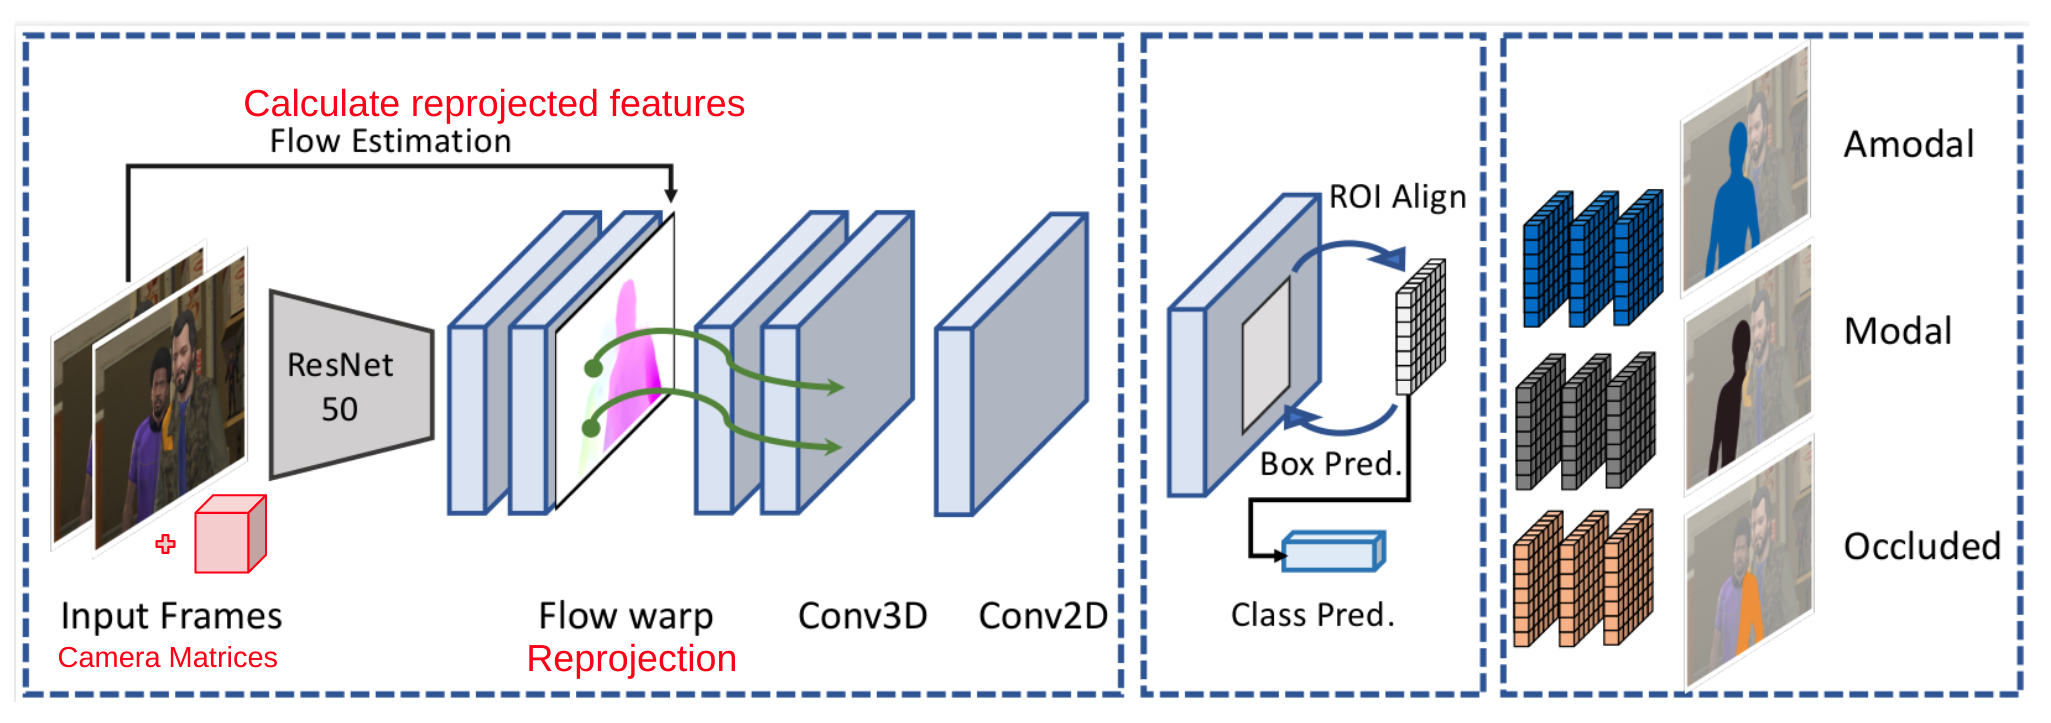
\includegraphics[width=0.97\textwidth]{fig/pipeline}
\vspace{-0.35cm}
\caption{Overview of our proposed framework for learning SAIL-VOS. Our Amodal-Net includes a temporal backbone, an iterative box-head and mask-head, while it is trained jointly with the task of modal and occlusion mask prediction.}
\vspace{-0.4cm}
\label{fig:pipeline}
\end{figure*}

Motivated by this capability, prior works~\cite{GuoECCV2012, SilbermanECCV2014b, KarICCV2015, LiECCV2016, zhu2017semantic, ehsani2018segan, follmann2019learning} studied the problem of amodal segmentation from a single image, \ie, the task of segmenting  both the visible \textit{and occluded} parts of an object.  
In meticulous work, Hu~\etal~\cite{hu2019sail} collected a dataset for  the task of Semantic Amodal Instance Level Video Object Segmentation (SAIL-VOS). Annotation of video data permits to expand amodal reasoning to the time dimension, which also seems crucial for human perception. However, the models proposed by Hu~\etal~\cite{hu2019sail} do not  take  advantage of the temporal information
and are mostly adapted from the modal instance segmentation task. 
While this is a very valuable first step, it is suboptimal for three reasons illustrated in. Specifically, missing temporal information prevents use of motion cues. Moreover, bounding boxes of amodal segmentations overlap much more significantly than those of modal masks. We found special treatment of this issue to improve results. In addition, amodal segmentation requires to deal with occlusions, \ie, object information from observations needs to be propagated more broadly.

To tackle these three challenges, Yeh and I proposed Amodal-Net, a framework for SAIL-VOS with a flow based temporal backbone, a redesigned box-head and a revised mask-head. 
More specifically, our temporal backbone enables the model to reason about occluded regions based on current and past frames. For this we incorporate temporal information into the amodal prediction model. Our box-head utilizes a cascade architecture with soft Non-Maximum Suppression (NMS) to address the challenge of heavily overlapping amodal boxes. Lastly, we developed a mask head with a large receptive field and self-attention to better propagate object information far into the occluded regions. 

Recently, Hu~\etal~\cite{HuCVPR2021} also collected detailed 3D information on SAIL-VOS. Intuitively, 3D information combined with temporal information will offer more clues for objects and their occlusion. Therefore, this thesis explores the effect of adding 3D information to the video data.  In particular, the model will incorporate depth maps and camera intrinsic and extrinsic matrices into the input, and perform 3D reprojection in the feature space.


We evaluate our approach on the SAIL-VOS dataset~\cite{hu2019sail}, where we outperform state-of-the-art by $3.5\%$ (absolute-gain) in Average Precision (AP) on amodal video instance segmentation. 
We also investigate the effect of reprojection on the accuracy of our model on the SAIL-VOS dataset. Compared to the repreojection-less 
model, adding reprojection yields a minor improvemenet in AP, as well as a more significant improvement of $0.2$ when restricted to small 
objects.

%In order to extend our proposed methods into the standard amodal instance segmentation task and 
Next, to assess the generality of \textit{non-temporal} components in the base model,
%To the best of our knowledge, %~\cite{hu2019sail} 
%this is the only available video dataset. 
%To assess the generality of the \textit{non-temporal} components in \ourmodel, 
we also report results on the COCO-Amodal dataset~\cite{zhu2017semantic} and the KINS dataset~\cite{qi2019amodal}.
Our approach outperforms state-of-the-art by 4.0\% AP and 1.1\% AP respectively.
%\as{refer to fig.~1 and some nice illustrations where thingsg work.}   % Inserts content from "introduction.tex" here

\chapter{Background}
\label{chp:bg}
%!TEX root = main.tex
In this chapter I will breifly review relevant concepts. First I will review works on instance segmentation, which are often a source of inspiration for amodal methods.
Subsequently I will discuss amodal segmentation. Lastly, I will review network architectures for extracting features from videos in other tasks, which serves as an inspiration for temporal data. 
\section{Instance Segmentation}

Instance segmentation is a long-standing goal in computer vision that requires the prediction of object instances and their per-pixel segmentation mask. This makes it a hybrid of semantic segmentation and object detection.
~\cite{BarinovaPAMI2012, RiemenschneiderECCV2012, KimCVPR2012, PinheiroNIPS2015, DaiCVPR2016, PinheiroECCV2016, DaiECCV2016, LiCVPR2017, liu2018path, fang2019instaboost, yolacticcv2019, lee2020centermask, Cao_D2Det_CVPR_2020, wang2020solo}.[TODO: maybe add more bg in instance segm and a picture that compares it with semestic segm] 

Mask-RCNN-based methods have shown strong results on instance segmentation~\cite{he2017mask, cai2018cascade, liu2018path, chen2019hybrid}. These detect-then-segment methods first extract image features via a backbone network, \eg, a ResNet. A Region Proposal Network (RPN)~\cite{ren2015faster} subsequently retrieves a set of candidate bounding boxes and their objectness scores. This is achieved by sliding a small convolutional network over the features extracted via the  backbone network. 

These candidates may  heavily overlap with each other. %, therefore 
To reduce redundant computation due to the overlap, Non-Maximum Suppression (NMS) or its soft-version Soft-NMS~\cite{bodla2017soft} is applied to filter   candidates. 

Given the candidate bounding boxes,  ROIAlign~\cite{he2017mask} is used to extract a feature map for each of the candidate boxes. The bounding box features are subsequently processed by a box-head and/or a mask-head, which regress to bounding box and segmentation mask respectively. The box-head consists of fully connected layers and yields a classification prediction and a  corresponding bounding box.  %the bounding box size and its location. 
The mask-head consists of a stack of convolutional layers, which yield a $28 \times 28$ class-specific mask. 

Variants of Mask-RCNN rely on a multi-stage refinement approach, \ie, a cascade is used to enhance the box-prediction accuracy~\cite{cai2018cascade, chen2019hybrid}. While our method also relies on a cascade design, our model is specifically designed for the task of SAIL-VOS. Different from these works, we propose a temporal backbone to aggregate information over time, Soft-NMS to handle overlapping amodal boxes, and an iterative mask-head with attention to propagate information into occluded regions. 

\section{Amodal Image/Instance Segmentation.}
Amodal instance segmentation is the task to delineate objects and their occluded parts in video or image data. The goal is to predict a mask for every object that is in the image, and the mask would draw out the whole object includding any part that may be occluded. 

Annotations for amodal segmentation are challenging to obtain due to  ambiguities caused by  occlusions. Early works~\cite{GuoECCV2012, GuptaCVPR2013, SilbermanECCV2014b, KarICCV2015} view the problem as a contour completion task. Other works~\cite{HsiaoCVPR2012, PepikCVPR2013, GhiasiCVPR2014, ChenCVPR2015, LiECCV2016}  formulate the problem as occlusion reasoning from a single image. Generally, the focus is on the class-agnostic setting, where the predicted segmentation consists of only two classes, either foreground or background. Maire \etal~\cite{maire2013hierarchical} collect one of the earliest datasets for amodal segmentation, labeling 100 images. %}
%\as{citations missing, e.g. Li and Malik; check Sail-VOS paper}

More recently, datasets with class annotations were released. For instance, Zhu~\etal~\cite{zhu2017semantic} introduce the COCO-A dataset, which adds amodal annotations to 5000  images from the COCO dataset~\cite{lin2014microsoft}. Even more recently, larger datasets for amodal segmentation have been collected. For example, Qi~\etal~\cite{qi2019amodal} collect amodal annotations for the KITTI dataset~\cite{geiger2012we}. Concurrently, Hu~\etal~\cite{hu2019sail} propose to use a game engine to automatically collect realistic  annotations for amodal segmentation of video data. The use of a game engine circumvents any accuracy concerns for amodal annotation, which is %commonly
challenging to obtain due to ambiguity. It hence avoids labor-intensive human labeling. Work by Hu \etal~\cite{hu2019sail} further enables to train and evaluate amodal instance segmentation on videos, \ie, the task of SAIL-VOS. Based on these datasets, Mask-RCNN-based methods for single image instance segmentation have been proposed~\cite{follmann2019learning, hu2019sail}. More specifically, Follman \etal~\cite{follmann2019learning} discuss a two mask-head approach, which yields the amodal mask, the modal mask, and a combination of both results to form the occlusion mask for end-to-end training on all three masks. Hu \etal~\cite{hu2019sail} propose to jointly train the amodal and modal mask. Different from these works, we consider input of videos and specifically design an architecture to address prevalent challenges for the task of SAIL-VOS.


\section{Video and Reprojection Architectures}
Capturing temporal information is also crucial for tasks involving any form of video understanding, \eg, video segmentation, recognition, inpainting, \etc. There are various methods to align features from different timestamps. For example, optical flow has been used as an additional deep-net input for video action recognition~\cite{simonyan2014two, singh2016first}. Other methods incorporate optical flow by warping images or features, aligning them to the current frame of interest~\cite{hu2017maskrnn,gadde2017semantic, kim2019deep}. In my previous work with Yeh, similar flow-based method was incorporated into the net. In this thesis we will use camera reprojection in the net for aligning features from different frames. Reprojection uses the intrinsic and extrinsic parameters of the camera to warp an image into the perspective of another image. Assuming the objects themselves move negliglibly between two consecutive frames, reprojection allows us to use temporal information from prior frames while processing a given frame. If the camera matrices are known, this provides a precise way to incorporate temporal information into the training architecture.


\chapter{Approach}
\label{chp:approach}
The first step of our approach is Amodal-net, an amodal framework illustrated in Fig.~\ref{fig:pipeline} without the red annotations. The next step is to try to incorporate 3D information into the data used for training, as shown in red annotations in Fig.~\ref{fig:pipeline}. Intuitively,  incorporating 3D information should allow the learning pipeline to use the temporal information better. For example, if the pipeline can see that an object is partialy blocked by an object that has a $z$ value, it should know to still map out the object in its whole shape in the amodal mask. 

The SAILVOS dataset~\cite{hu2019sail} has annotations for the depth map. The SAIL-VOS 3D dataset from Hu \etal \cite{HuCVPR2021} also contains camera intrinsics and extrinsics stored in the object files. Although there are some scene mismatches on the scale of a few milliseconds, I will nevertheless use these annotations to do mask reprojections in the data training pipeline.

\section{Overview}
Given a sequence of $T$ images $\mI_{t-T:t}=(\mI_{t-T+1}, \hdots, \mI_{t})$ our goal is to predict for each object $o\in\gO_t$ in the current frame $\mI_t$ the corresponding amodal mask $\mM_{t,o}$. 
%set of amodal segmentation masks, \ie, $\gM = \{\mM_{t,o}~\forall o \in \gO_t\}$, where $\mM_{t,o}$ is the amodal mask for object $o\in\gO_t$ in the $t^\text{th}$ frame $\mI_t$, and 
We let $\gO_t$ denote the set of detected objects in frame $\mI_t$, while $\gM_t = \{\mM_{t,o}~\forall o \in \gO_t\}$ refers to the set of segmentation masks.

To accomplish this goal, we first extract features $\phi_t$ for all $T$ frames in $\mI_{t-T:t}$. %We then use
Next, reprojection is used to spatially align features with the current frame $\mI_t$ via warping. We then perform spatial and temporal aggregation to compute the feature $\Phi_t$. This ensures that the backbone feature $\Phi_t$ summarizes temporal information. 

Next, our cascade Soft-NMS box-head detects objects and crops $\Phi_t$ to extract object-level features $\Phi_{t,o}$ for each detected object $o\in\gO_t$. Our box-head uses soft-thresholding during non-maximum suppression to better handle overlapping boxes. Given the object-level features $\Phi_{t,o}$, the amodal mask $\mM_{t,o}$ for each object is predicted using an iterative mask-head. We incorporate a large receptive field and self-attention into the iterative mask-head. % using a large receptive field and self-attention. 
Because of this, information can propagate across the entire detection during mask prediction.

\section{Amodal-Net}
The base model  `Amodal-Net' builds on top of Mask R-CNN~\cite{he2017mask}. Given the candidate bounding boxes, ROIAlign~\cite{he2017mask} is used to extract a feature map for each of the candidate boxes. The bounding box features are subsequently processed by a box-head and/or a mask-head, which regress to bounding box and segmentation mask respectively. The box-head consists of fully connected layers and yields a classification prediction and a  corresponding bounding box.  %the bounding box size and its location. 
The mask-head consists of a stack of convolutional layers. 

Variants of Mask-RCNN rely on a multi-stage refinement approach, \ie, a cascade is used to enhance the box-prediction accuracy~\cite{cai2018cascade, chen2019hybrid}. While our method also relies on a cascade design, our model is specifically designed for the task of SAIL-VOS. Amodal-net that Yeh and I developed with collaborator uses a temporal backbone to aggregate information over time, Soft-NMS to handle overlapping amodal boxes, and an iterative mask-head with attention to propagate information into occluded regions, as shown in Fig.~\ref{fig:pipeline}. We also found that multi-task training with the occlusion prediction task further improves performance. Combining the aforementioned techniques results in the following framework, for which a pictorial sketch is shown in~\figref{fig:pipeline}. This multi-task training is only included in the experiments for the Amodal-net and not included in the experiments with 3D Reprojection due to limitations in computation resources.

The changes in Amodal-net are made to address three challenges in this task: 
\begin{enumerate}
    \item[\bf (i)] limited use of temporal information;
    \item[\bf (ii)] missing mechanism to handle heavily overlapping amodal boxes; 
    \item[\bf (iii)] propagation of object observations which is often too short-sighted. 
\end{enumerate}

Amodal-net is based on {\bf (i)} a temporal backbone which aggregates information across video frames, {\bf (ii)} a box-head which 
better adjusts to overlapping detection boxes by using a cascade architecture with  Soft-NMS, 
and {\bf (iii)} a mask-head with increased receptive field and self-attention to propagate observations more broadly. Each of these components addresses the corresponding  challenge. 

One challenge in amodal box prediction is that it requires reasoning about the object size and shape despite occlusions. Importantly, different from the modal setting, an amodal box’s ground-truth more frequently overlaps with boxes de-lineating other detected objects. \figref{fig:sailvos_iou_hist} verifies this observation. To avoid non-maximum suppresion from removing boxes incorrectly due to heavier occlusion, cascaded soft NMS is used.

%!TEX root = main.tex

\begin{figure}[t]
\centering
\setlength{\tabcolsep}{0pt}
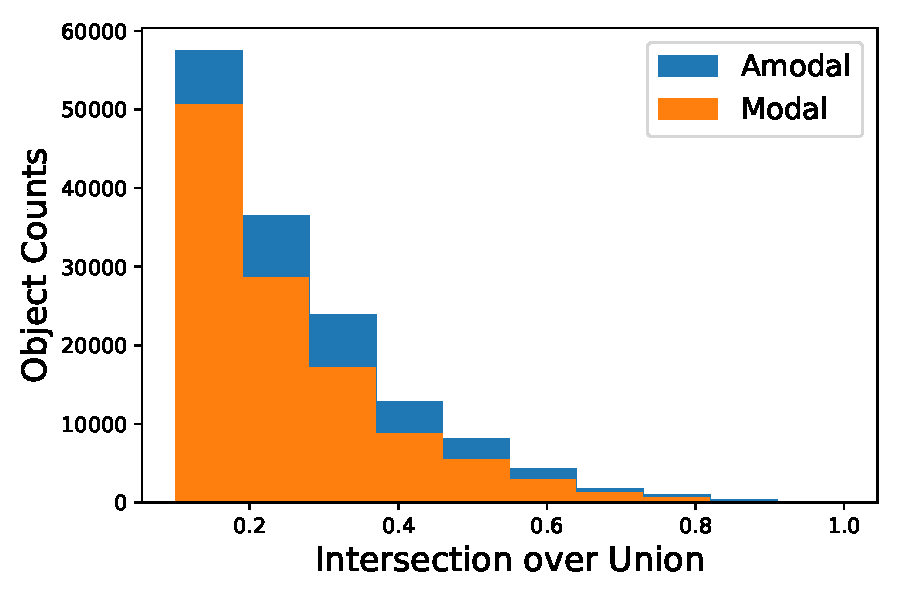
\includegraphics[width=0.48\linewidth]{fig/sailvos_iou_hist}
\vspace{-0.4cm}
\caption{Histogram of intersection over union (IoU) for Amodal and Modal boxes.}
\label{fig:sailvos_iou_hist}

\end{figure}


\section{3D Reprojection}
Following the aforementioned intuition, 3D reprojection is added in the pipeline to align inputs in the temporal dimension, as shown in red in \figref{fig:pipeline}. In the input, along with the images from frames $t$ and $t-1$, the camera matrices and the depth map of the corresponding frames are also passed in. The camera matrices include the intrinsic and extrinsic matrices of the camera.

The depth map and the camera matrices together are used to do reprojections from one frame to another. Standard computer vision reprojection algorithm warps an image from the perspective of one image to the perspetive of another image.

Given the image and the depth values of every pixel, we can get the camera coordinates for each pixel $X_{cam}$. For example, \figref{fig:3Dproj} plots one image in 3D camera coordinates. Then it is possible to calculate the camera coordinates of every pixel in another frame by using the camera matrices. $$ X_{cam} = K[R|t]X_{world} $$ where $K$ is the intrinsic matrix and $[R|t]$ is the extrinsic matrix representing rotation and translation of the camera. If we have two cameras looking at the same scene, $$X_{cam2} = K_2[R_2|t_2](K_1[R_1|t_1])^{-1}X_{cam1}$$ Finally, we can use $X_{cam2}$ to recover the pixel coordinates and thus get the reprojected image in 2 dimensions. One complication in implementation is that initially I was not sure what format the depth map is stored in. After consulting with authors of \cite{hu2019sail} and some exploration, I discovered that the data is stored in a variation of the normalized device coordinate (NDC) format. Hence camera coordinates of the image $X_{cam}$ had to be computed from NDC coordinates $X_{ndc}$. The details of the implementation are shown in \figref{apx:reproj}. 

I also experimented with estimating the camera matrices from the 2D and 3D points correspondence. However, due to the nature of how the data is collected in GTA-V and the format of the depth map, the estimated camera matrices induce a large error in reprojection compared to the ground truth camera matrices. In the end, I decided to use the ground truth matrices recorded. 

We can perform reprojection in image frames or masks. \figref{fig:reproj_image} shows an example of the reprojected image frame in full, and \figref{fig:reproj_mask} shows some examples of reprojected masks. In these plots, the first picture is the ground truth image of frame $t$; the second picture is the groundtruth image of frame $t-2$; the third picture is the groundtruth mask of an object at frame $t$; the fourth picture is the mask of the object at $t-2$ reprojected into the perspective of frame $t$; the last picture is the mask of the object at frame $t-2$ directly. The caption shows intersection over union of the last two masks with the groundtruth mask, \ie, the third mask. The reprojected image and mask should provide accurate information of the scene in previous frames since reprojection compensates for the movement of the camera. But there is one drawback to this approach: it does not take into account the movement of the object itself in the scene. If the object is also moving, the reprojected image would not reflect that. But as we can see from the captions of \figref{fig:reproj_image}, in general the reprojected mask is closer to the ground truth mask than directly using the mask from the prior frame, especially for objects that are still. 

In the network, we use the same algorithm but perform reprojection on the features of images produced by the backbone. By doing so, the features from different temporal indices are aligned in the sense that there are from the same perspective, and each pixel corresponds to the same spatial location. For this purpose, the depth map is reshaped into different shapes in the network to match the dimension of the features in the feature pyramid.

\begin{figure}

\centering
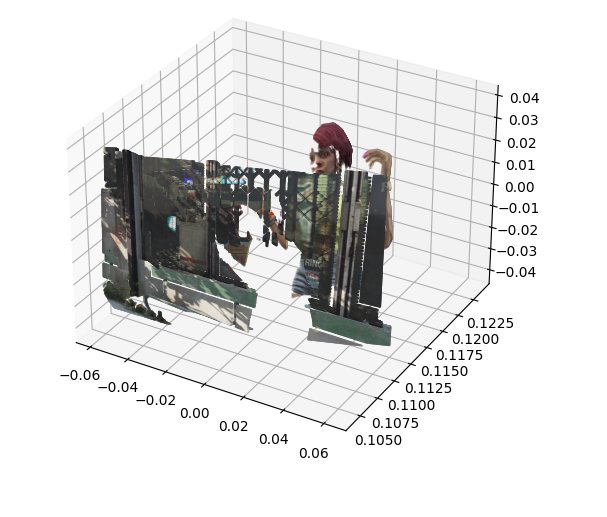
\includegraphics[scale=0.5]{fig/3dproj.png}
\caption{Projection of a frame in 3D camera coordinates.}
\label{fig:3Dproj}
\end{figure}


\begin{figure}
\centering
\begin{subfigure}[t]{0.19\textwidth}
\centering
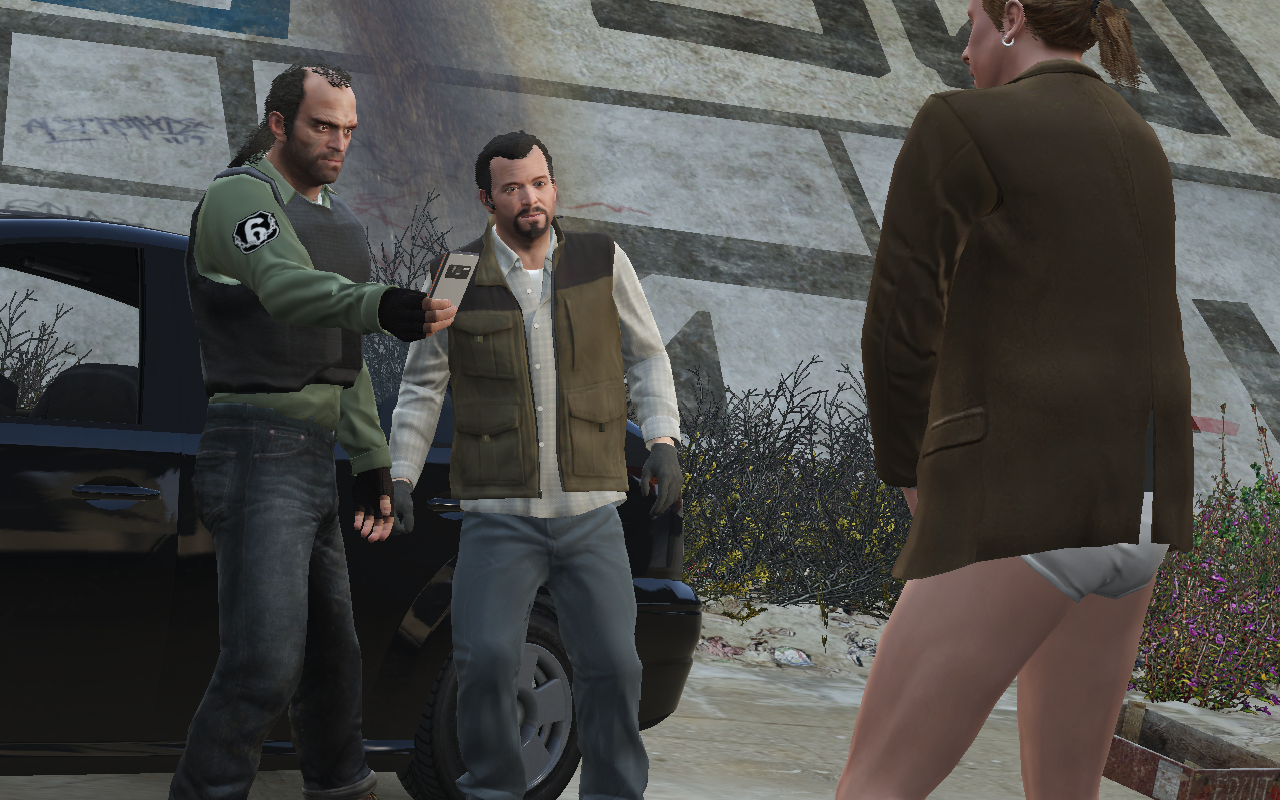
\includegraphics[scale=0.07]{good_examples/visual_179486_img.png}
\end{subfigure}
\begin{subfigure}[t]{0.19\textwidth}
\centering
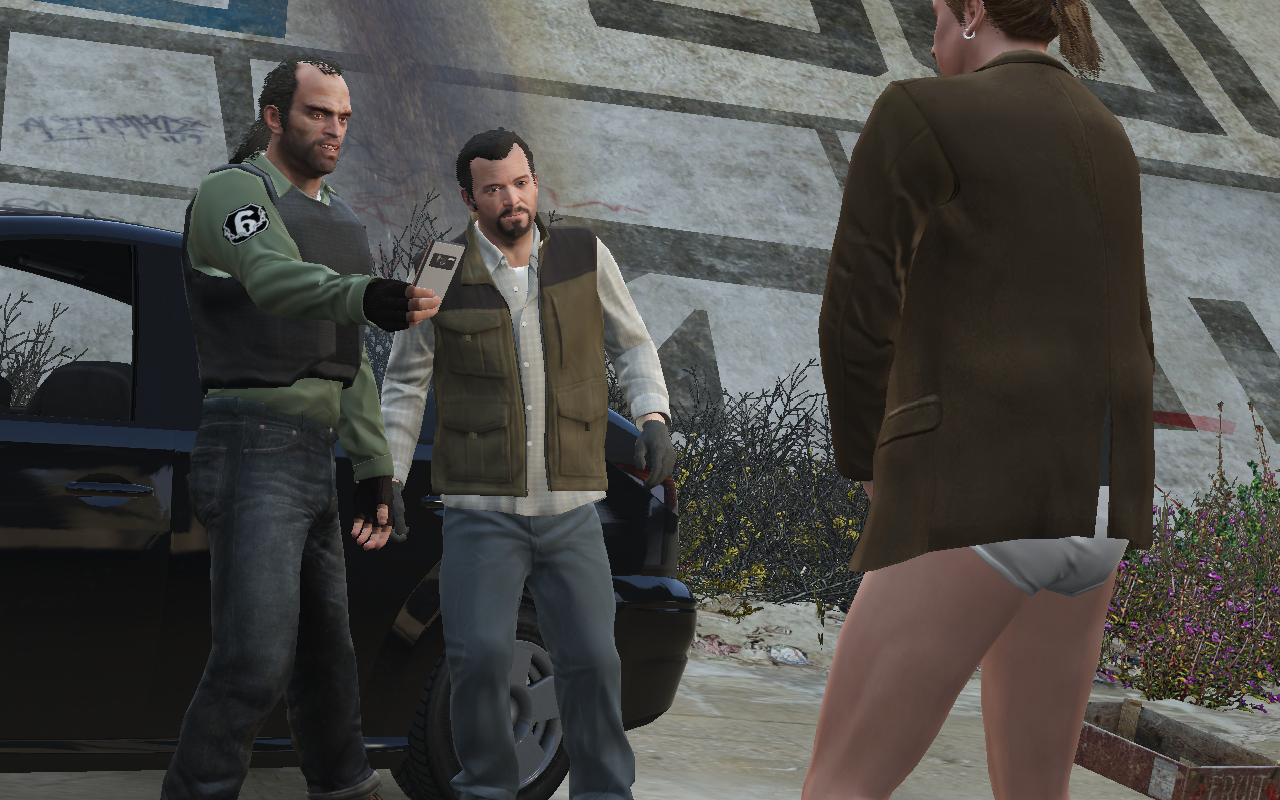
\includegraphics[scale=0.07]{good_examples/visual_179486_img1.png}
\end{subfigure}
\begin{subfigure}[t]{0.19\textwidth}
\centering

\includegraphics[scale=0.07]{good_examples/visual_179486_gt.png}
\end{subfigure}
\begin{subfigure}[t]{0.19\textwidth}
\centering
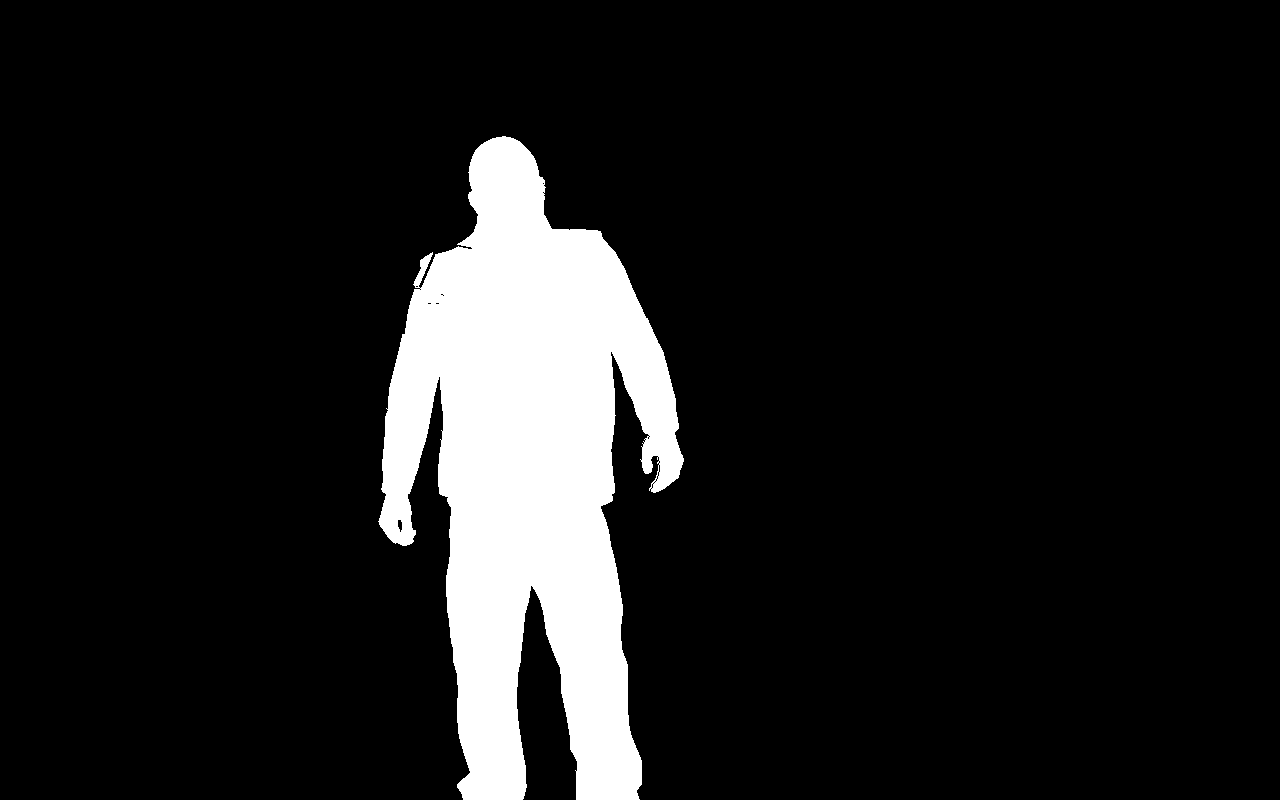
\includegraphics[scale=0.07]{good_examples/visual_179486_w_np.png}
\end{subfigure}
\begin{subfigure}[t]{0.19\textwidth}
\centering
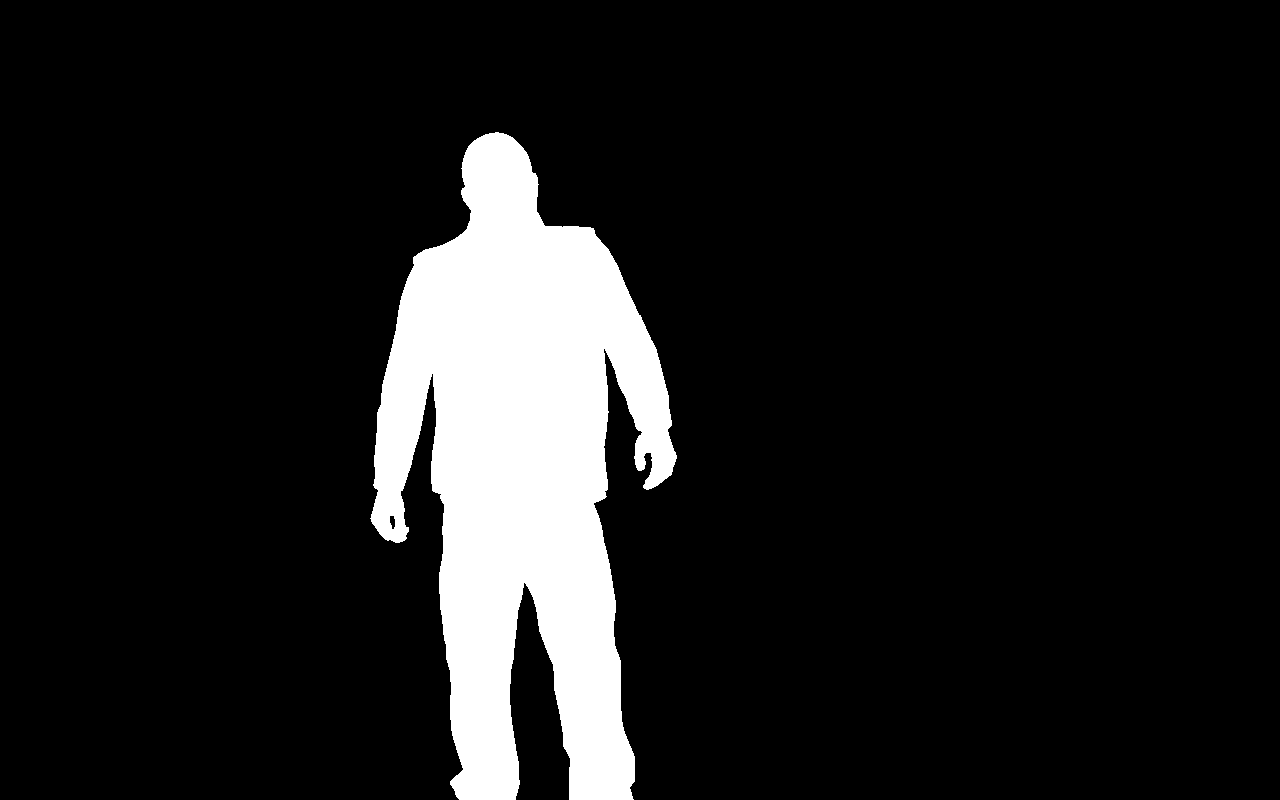
\includegraphics[scale=0.07]{good_examples/visual_179486_wo_np.png}
\end{subfigure}
\caption{IOU with reprojection: 0.85, IOU without reprojection: 0.75, video\_name: family\_4\_mcs\_3\_concat, frame\_number: 605.}
\label{fig:reproj_mask}
\end{figure}

\begin{figure}
\centering
\begin{subfigure}[t]{0.19\textwidth}
\centering
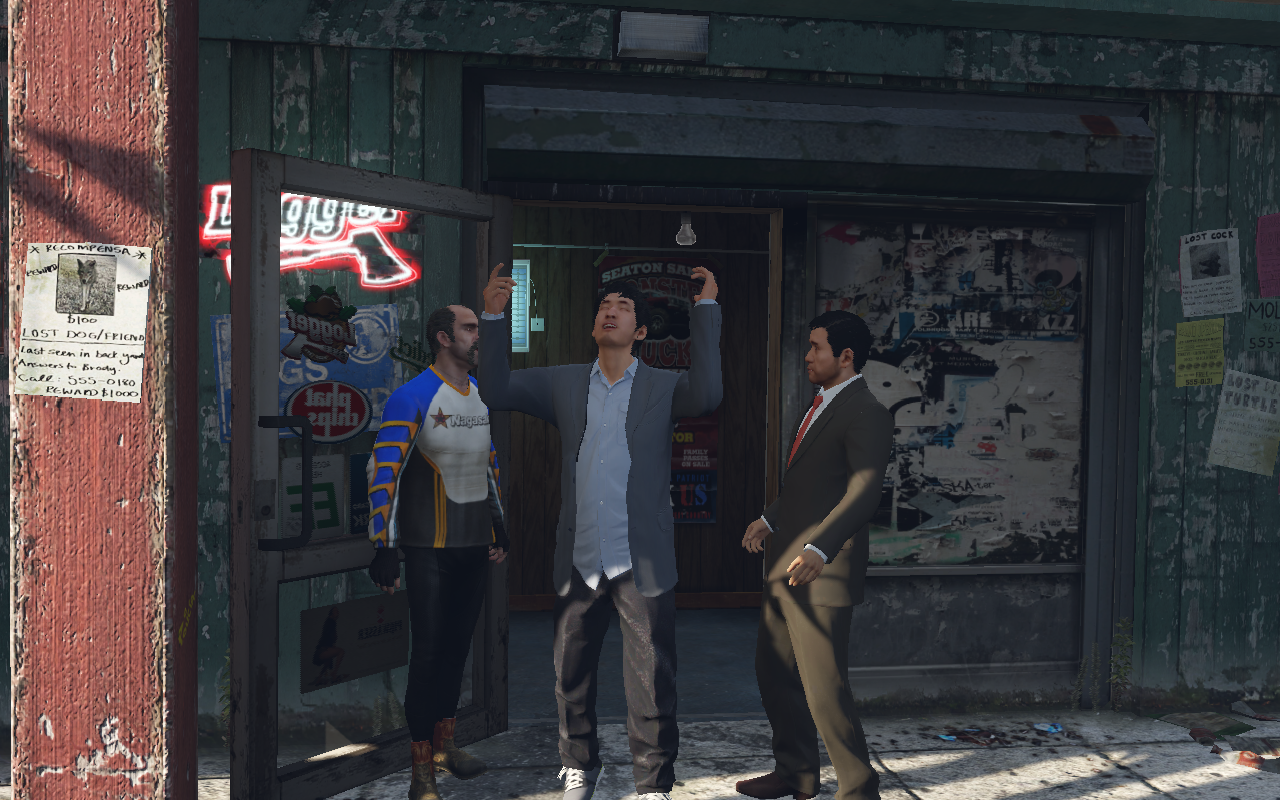
\includegraphics[scale=0.07]{good_examples/visual_74577_img.png}
\end{subfigure}
\begin{subfigure}[t]{0.19\textwidth}
\centering
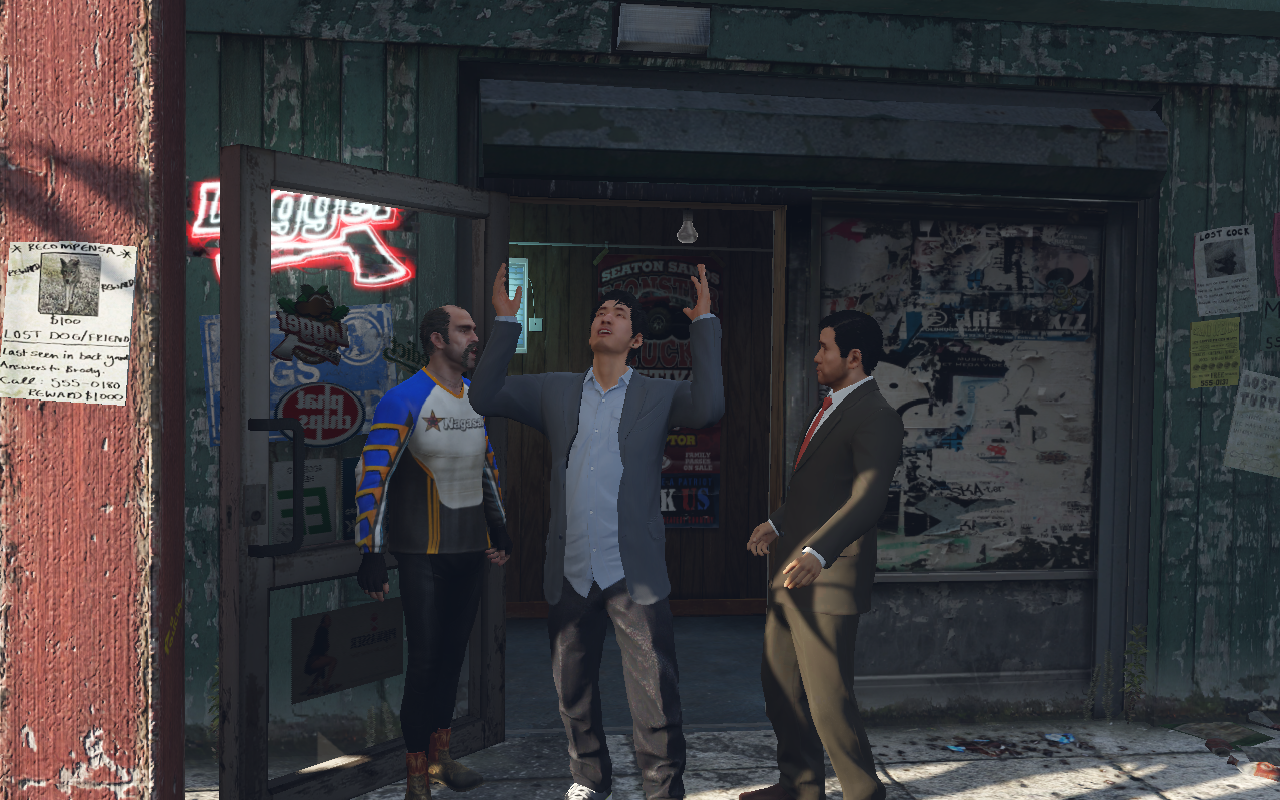
\includegraphics[scale=0.07]{good_examples/visual_74577_img1.png}
\end{subfigure}
\begin{subfigure}[t]{0.19\textwidth}
\centering
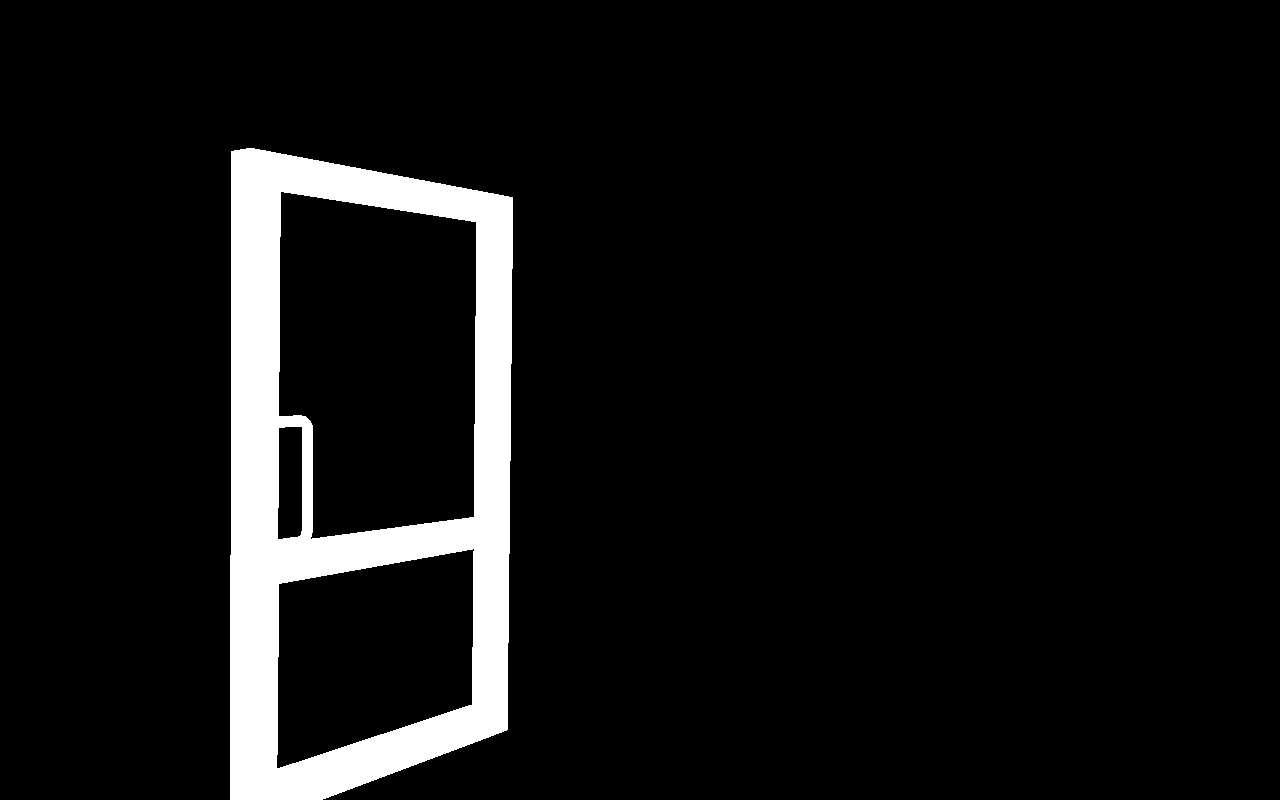
\includegraphics[scale=0.07]{good_examples/visual_74577_gt.png}
\end{subfigure}
\begin{subfigure}[t]{0.19\textwidth}
\centering
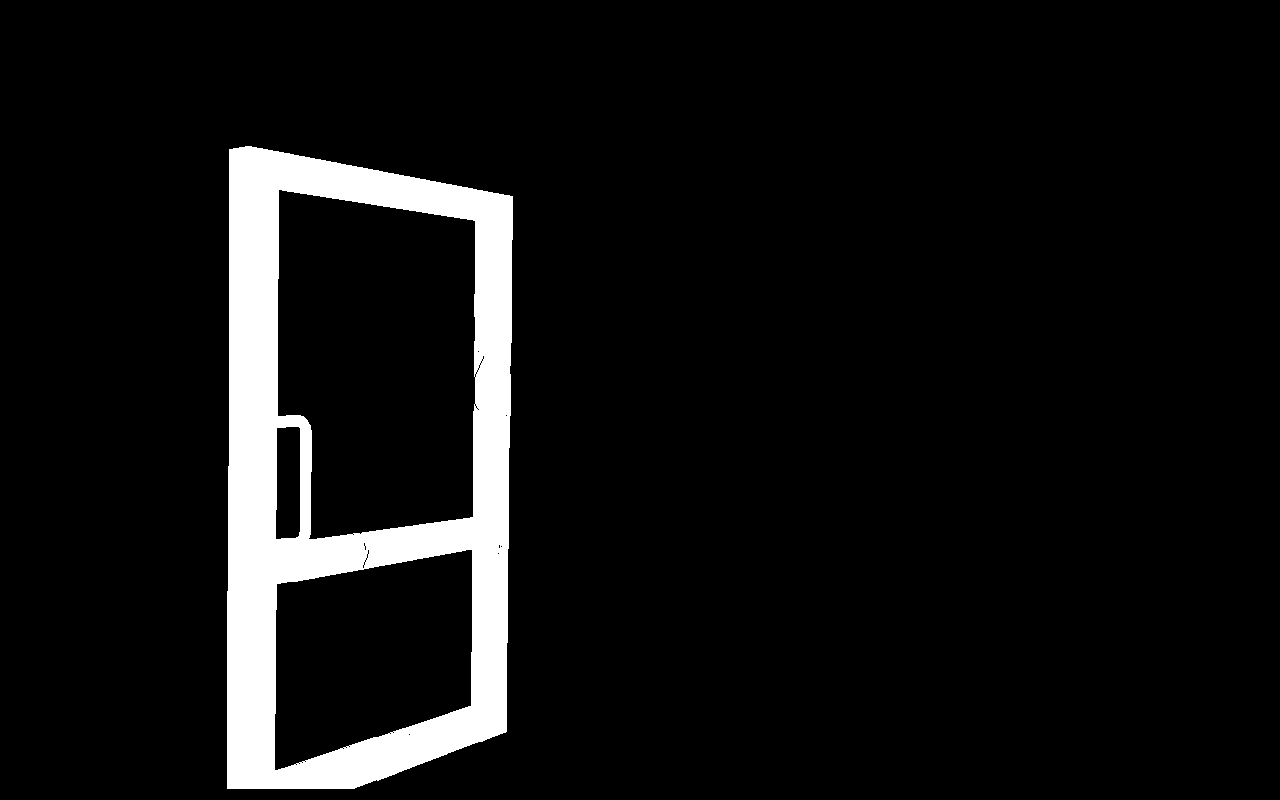
\includegraphics[scale=0.07]{good_examples/visual_74577_w_np.png}
\end{subfigure}
\begin{subfigure}[t]{0.19\textwidth}
\centering
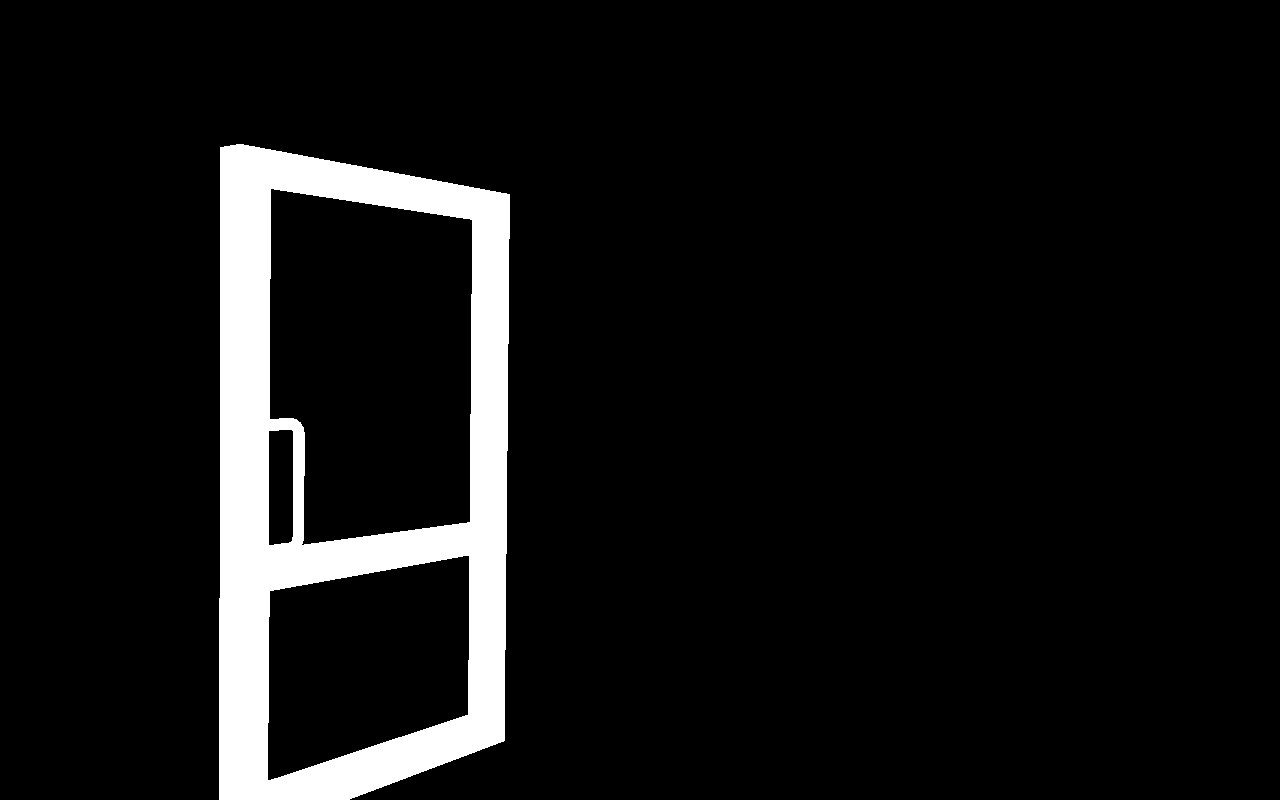
\includegraphics[scale=0.07]{good_examples/visual_74577_wo_np.png}
\end{subfigure}
\caption{IOU with reprojection: 0.91, IOU without reprojection: 0.72, video\_name: chinese\_1\_int, frame\_number: 978.}
\end{figure}

\begin{figure}
\centering
\begin{subfigure}[t]{0.19\textwidth}
\centering
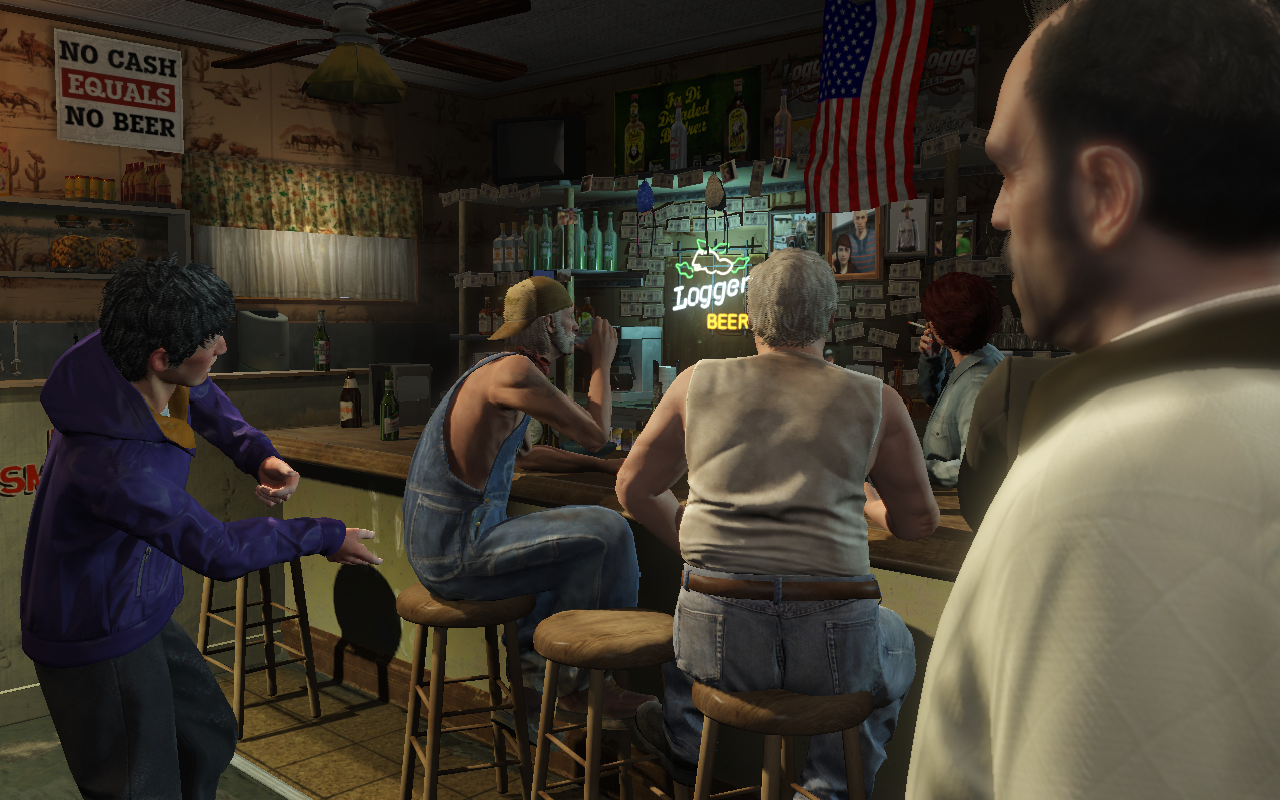
\includegraphics[scale=0.07]{good_examples/visual_76165_img.png}
\end{subfigure}
\begin{subfigure}[t]{0.19\textwidth}
\centering
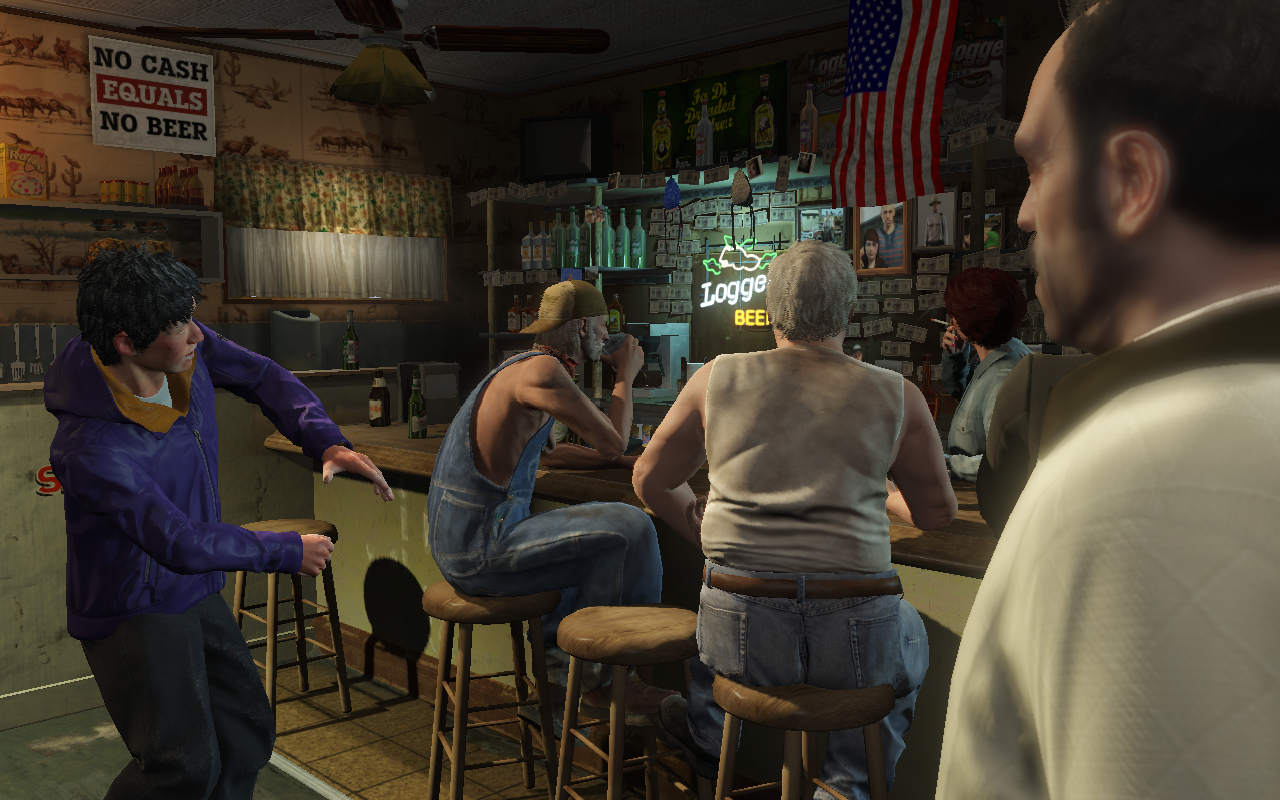
\includegraphics[scale=0.07]{good_examples/visual_76165_img1.png}
\end{subfigure}
\begin{subfigure}[t]{0.19\textwidth}
\centering
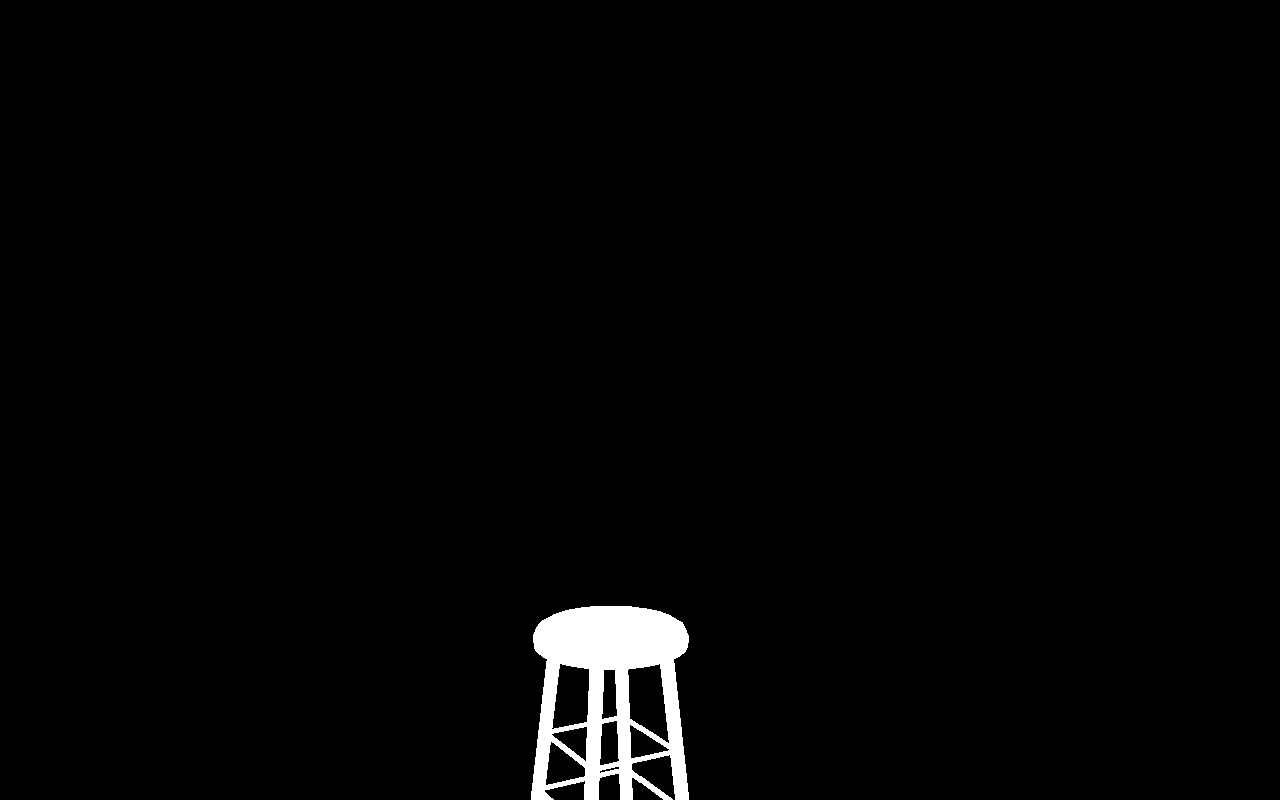
\includegraphics[scale=0.07]{good_examples/visual_76165_gt.png}
\end{subfigure}
\begin{subfigure}[t]{0.19\textwidth}
\centering
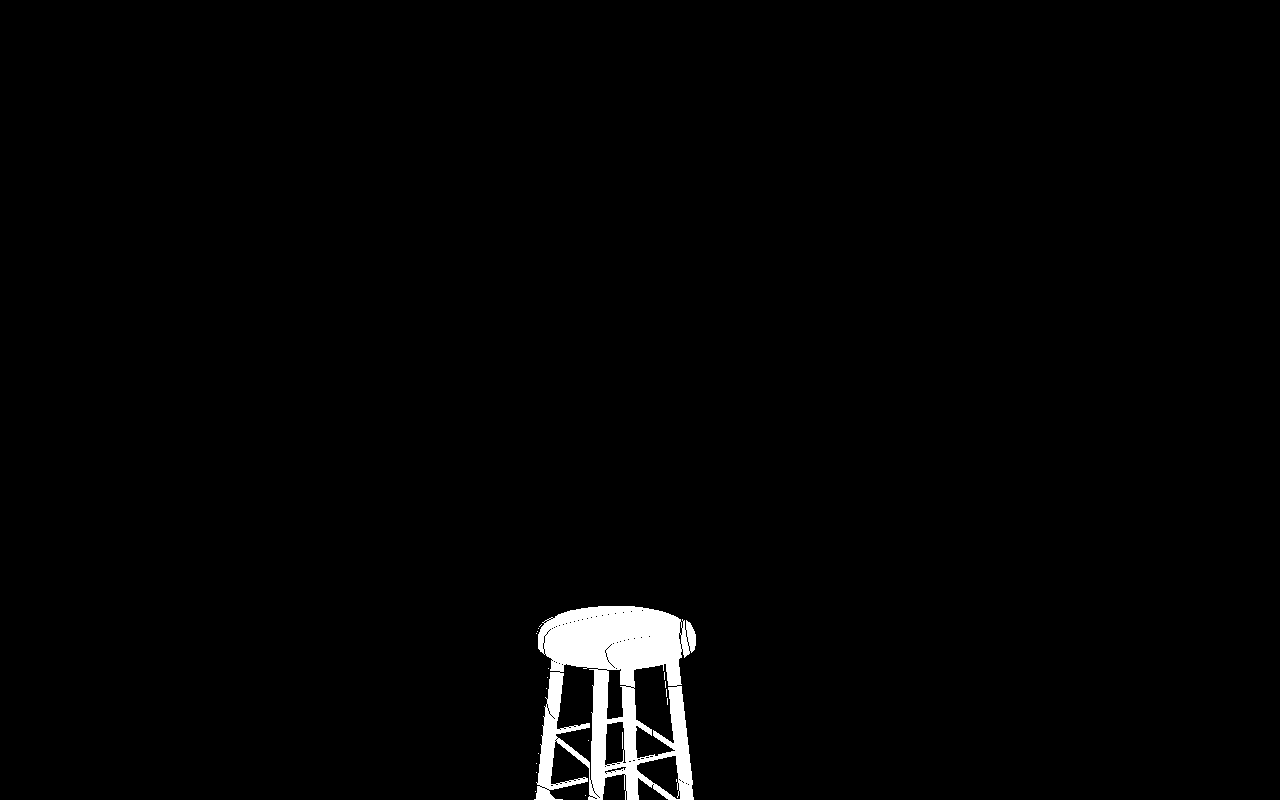
\includegraphics[scale=0.07]{good_examples/visual_76165_w_np.png}
\end{subfigure}
\begin{subfigure}[t]{0.19\textwidth}
\centering
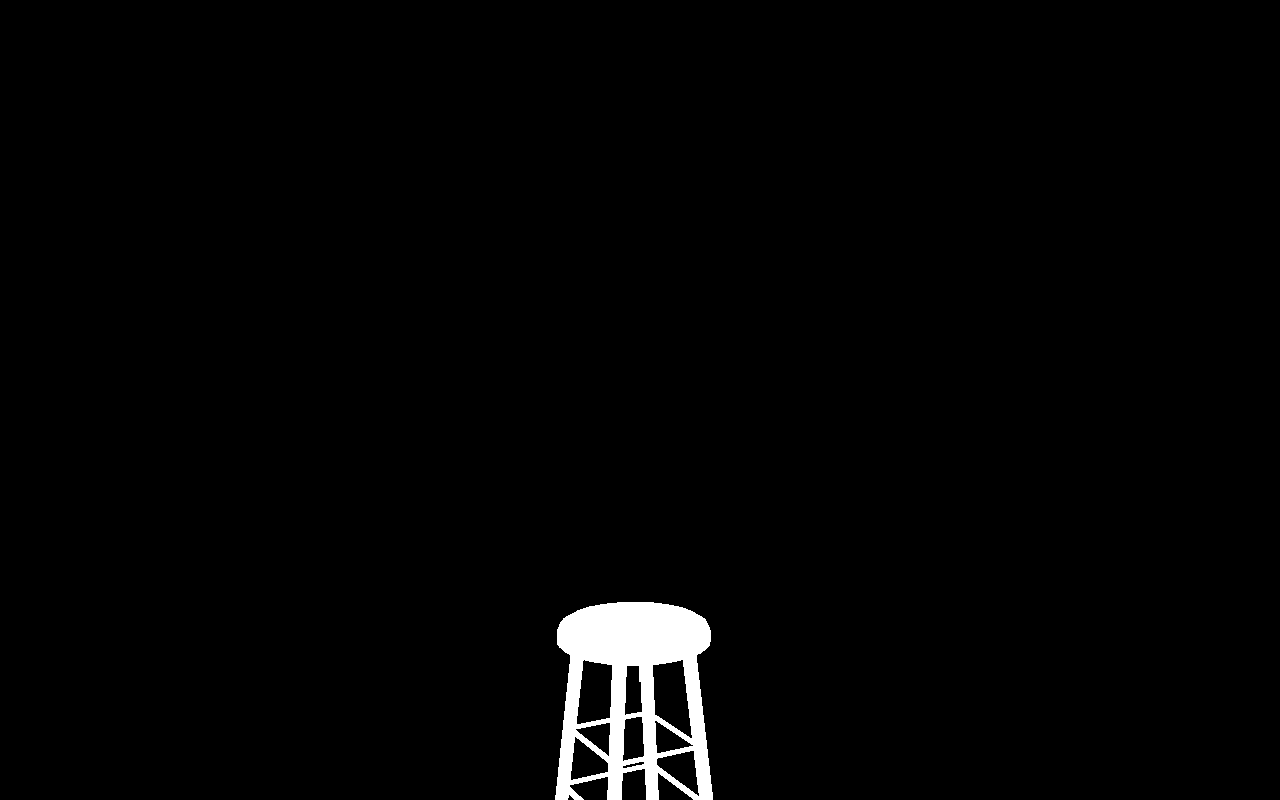
\includegraphics[scale=0.07]{good_examples/visual_76165_wo_np.png}
\end{subfigure}
\caption{IOU with reprojection: 0.67, IOU without reprojection: 0.36, video\_name: chinese\_2\_int, frame\_number: 67.}
\end{figure}


\begin{figure}
\centering
\begin{subfigure}[t]{0.19\textwidth}
\centering
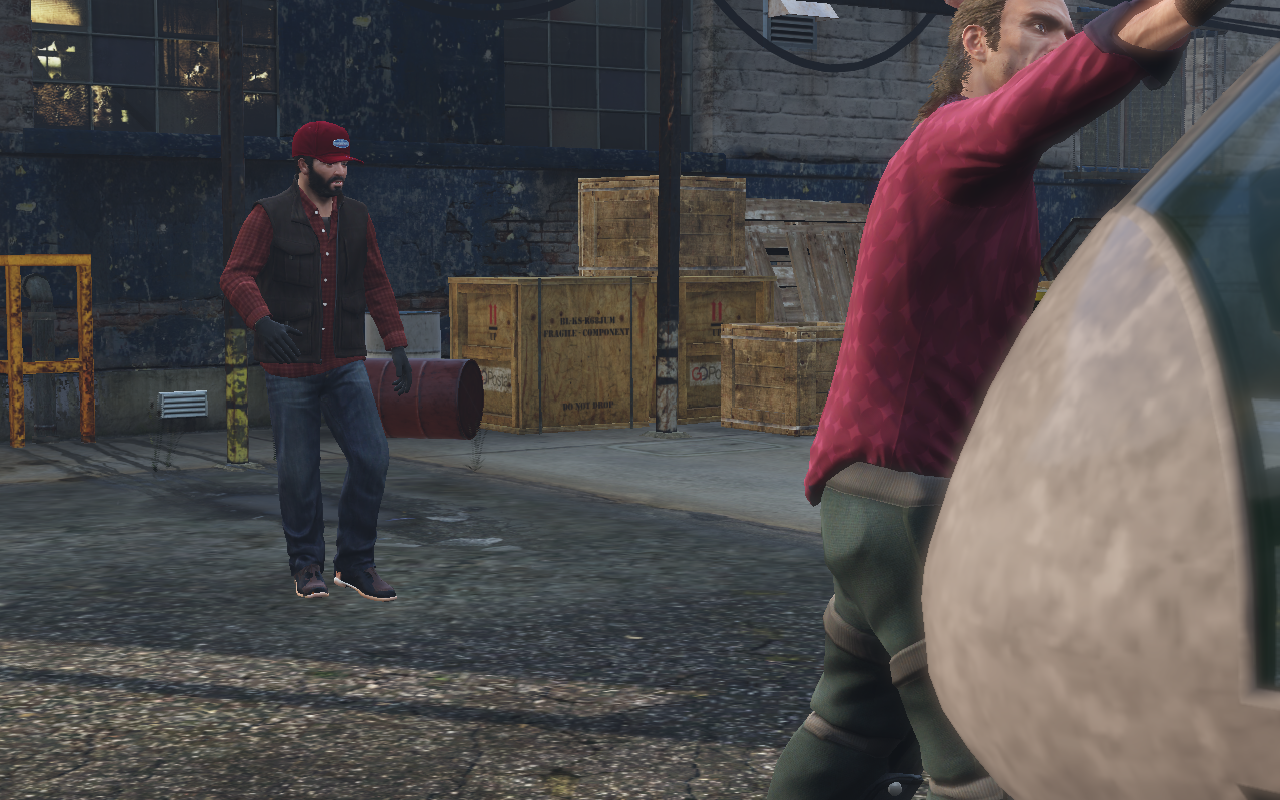
\includegraphics[scale=0.07]{good_examples/visual_211770_img.png}
\end{subfigure}
\begin{subfigure}[t]{0.19\textwidth}
\centering
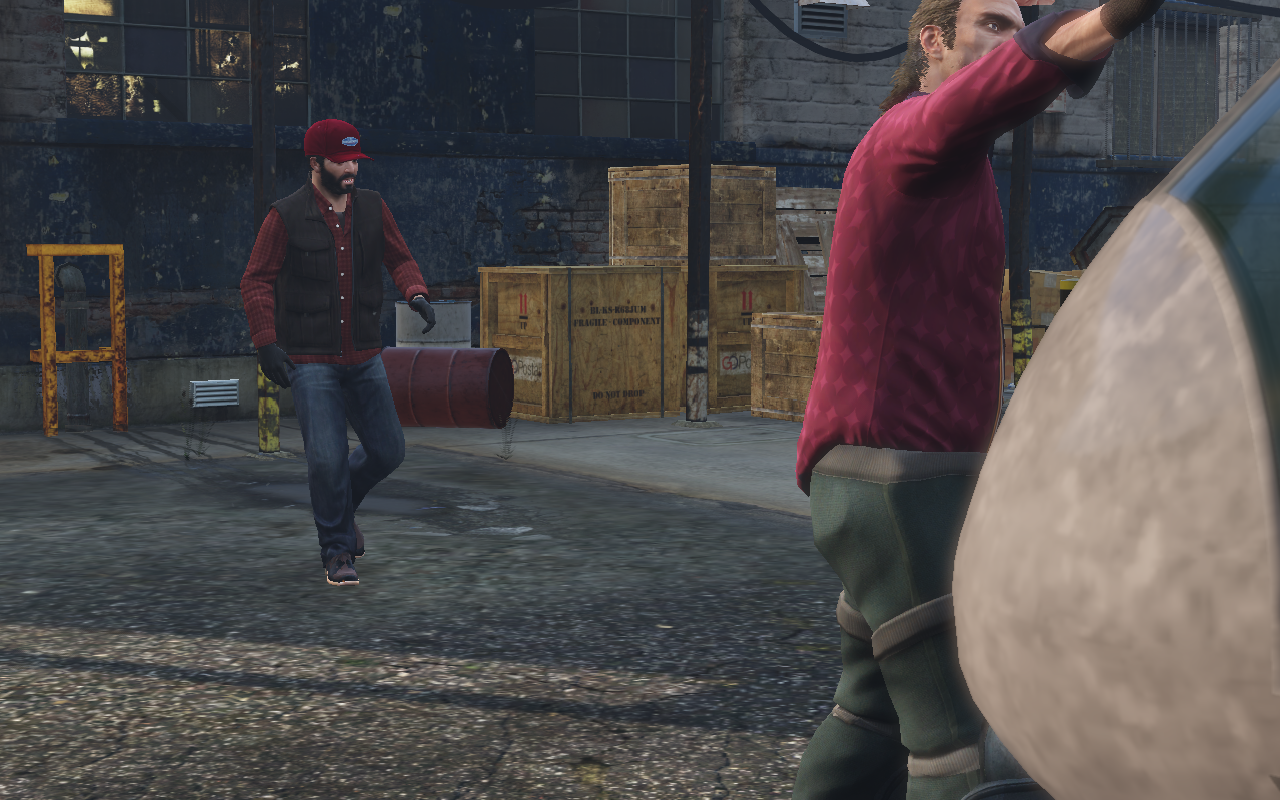
\includegraphics[scale=0.07]{good_examples/visual_211770_img1.png}
\end{subfigure}
\begin{subfigure}[t]{0.19\textwidth}
\centering
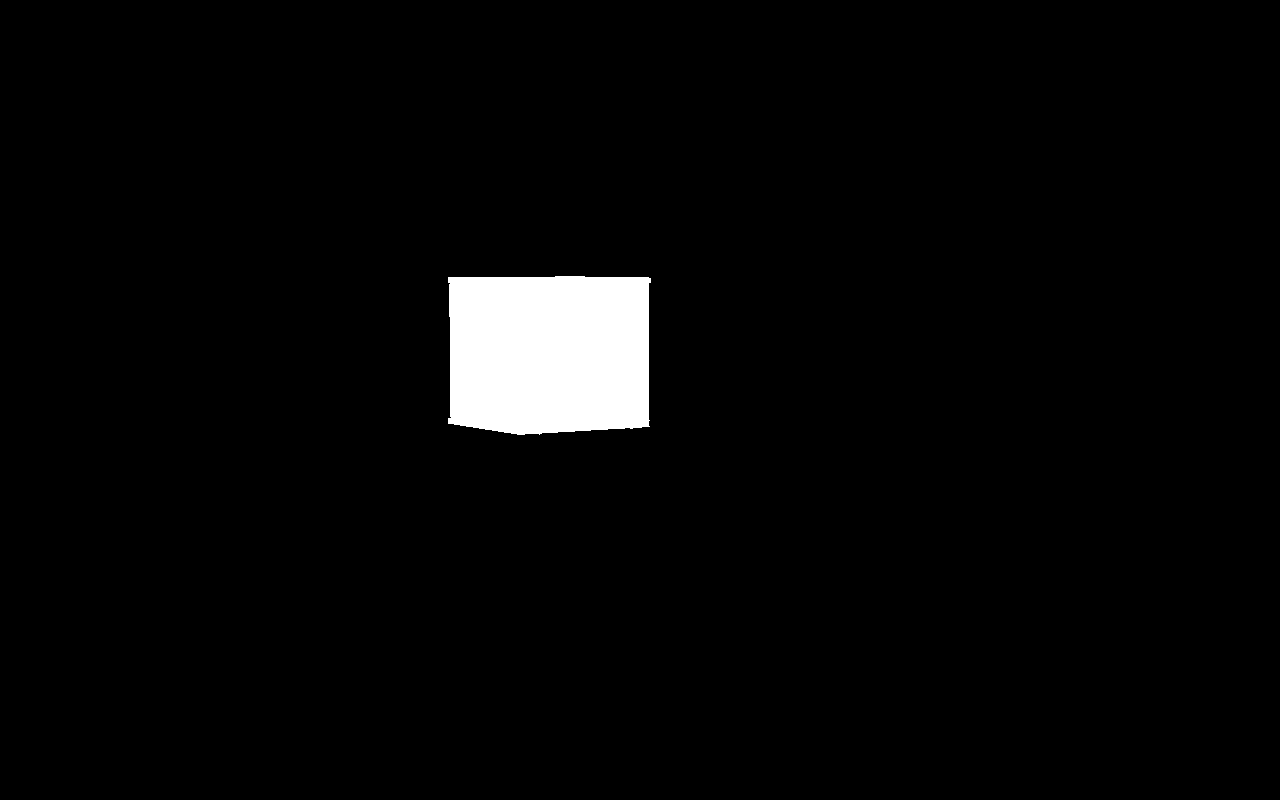
\includegraphics[scale=0.07]{good_examples/visual_211770_gt.png}
\end{subfigure}
\begin{subfigure}[t]{0.19\textwidth}
\centering
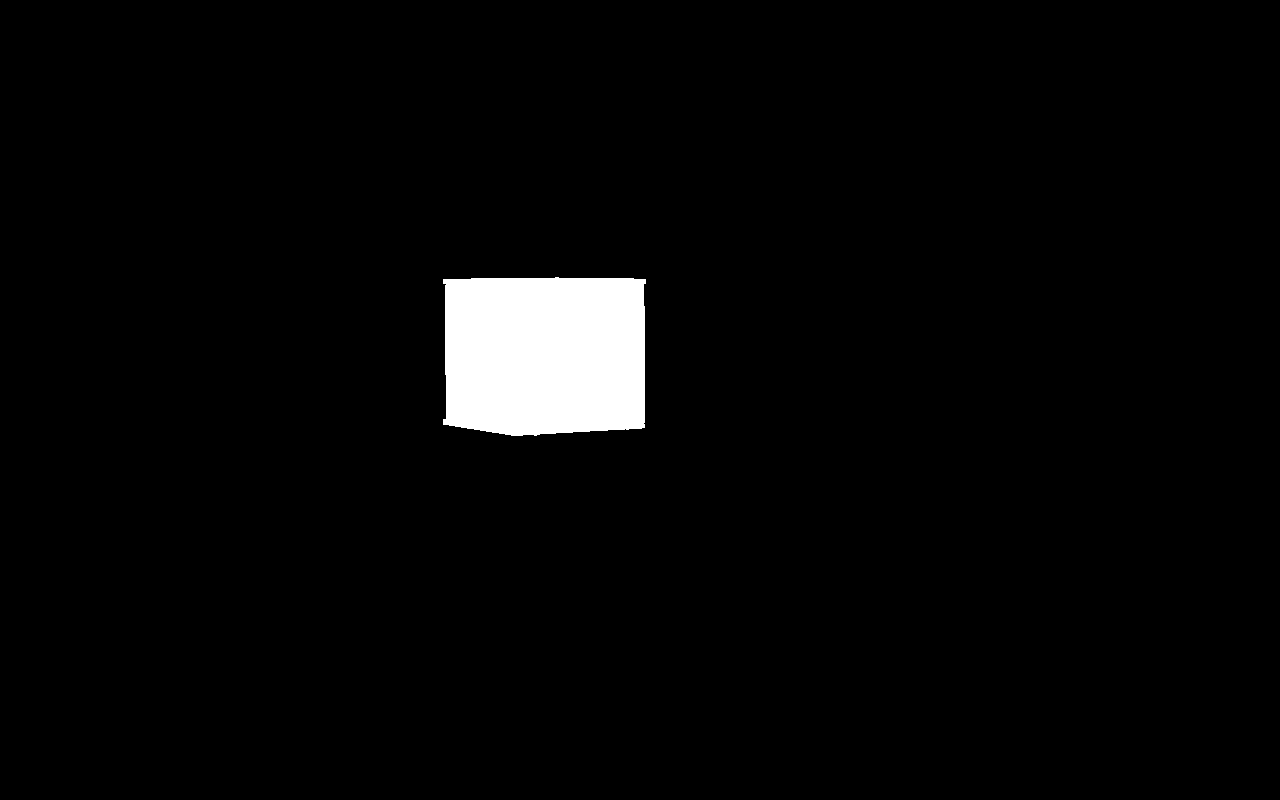
\includegraphics[scale=0.07]{good_examples/visual_211770_w_np.png}
\end{subfigure}
\begin{subfigure}[t]{0.19\textwidth}
\centering
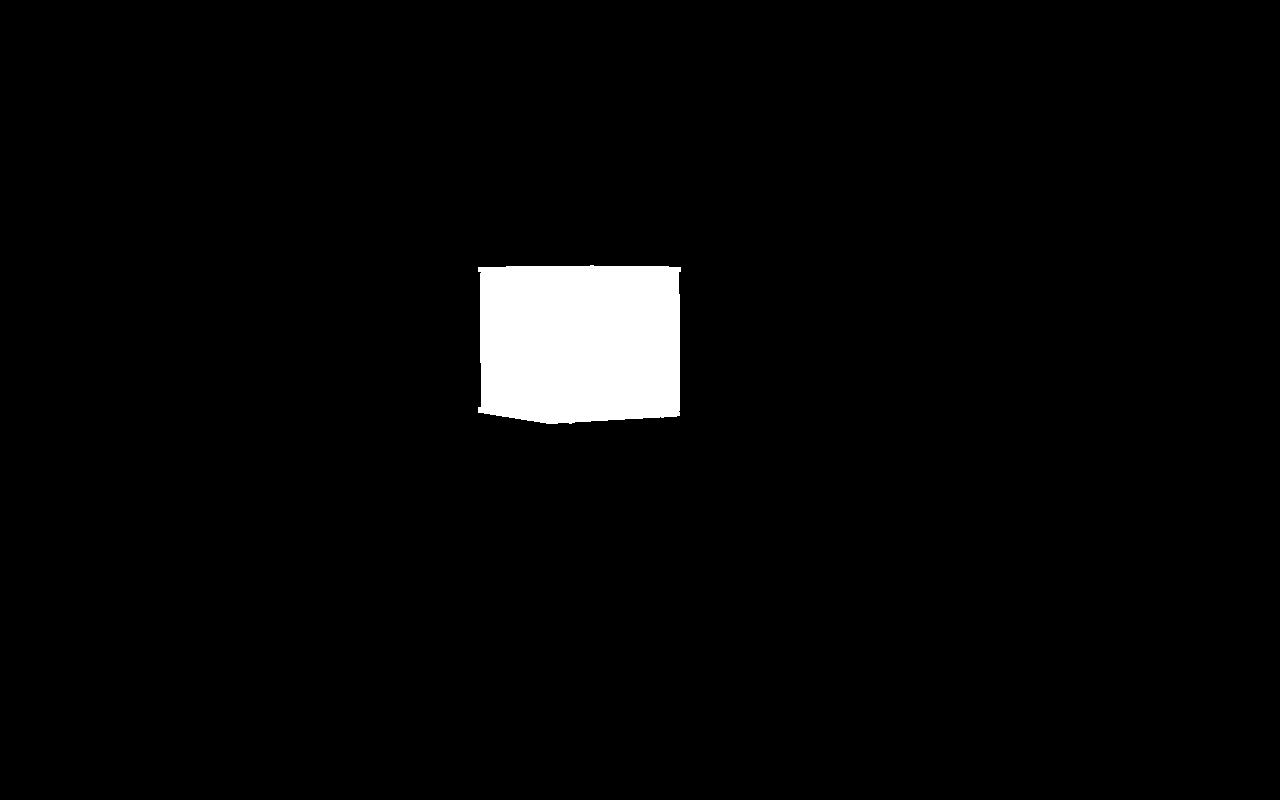
\includegraphics[scale=0.07]{good_examples/visual_211770_wo_np.png}
\end{subfigure}
\caption{IOU with reprojection: 0.94, IOU without reprojection: 0.65, video\_name: fbi\_2\_ext, frame\_number: 278.}
\end{figure}
\begin{figure}
\centering
\begin{subfigure}[t]{0.19\textwidth}
\centering
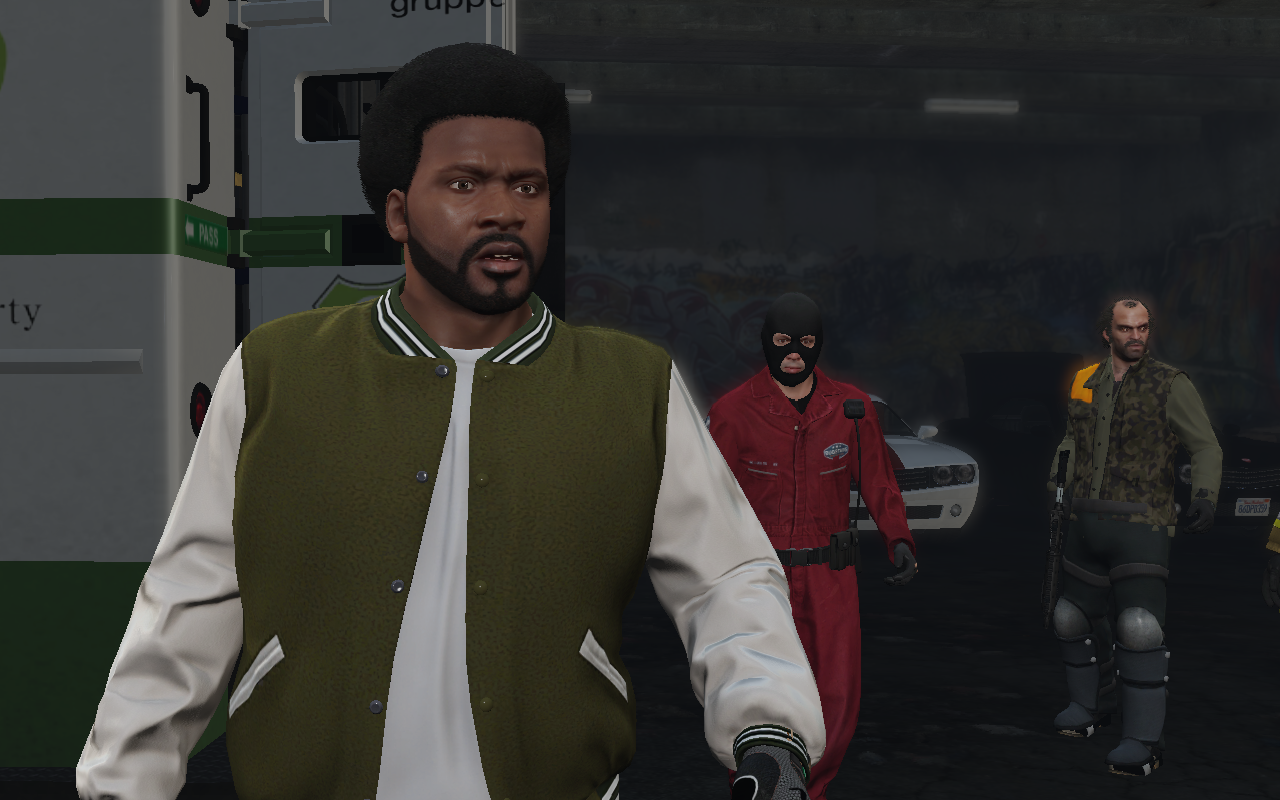
\includegraphics[scale=0.07]{good_examples/visual_29224_img.png}
\end{subfigure}
\begin{subfigure}[t]{0.19\textwidth}
\centering
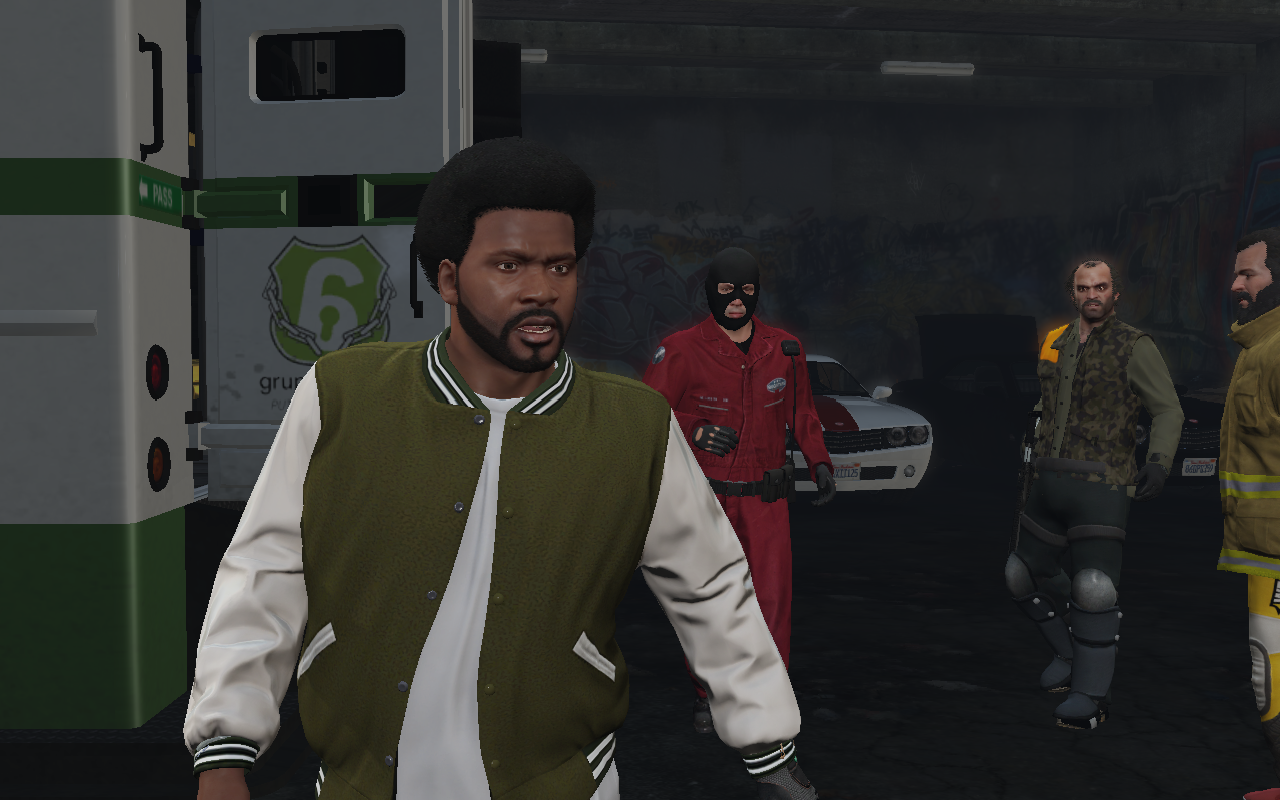
\includegraphics[scale=0.07]{good_examples/visual_29224_img1.png}
\end{subfigure}
\begin{subfigure}[t]{0.19\textwidth}
\centering
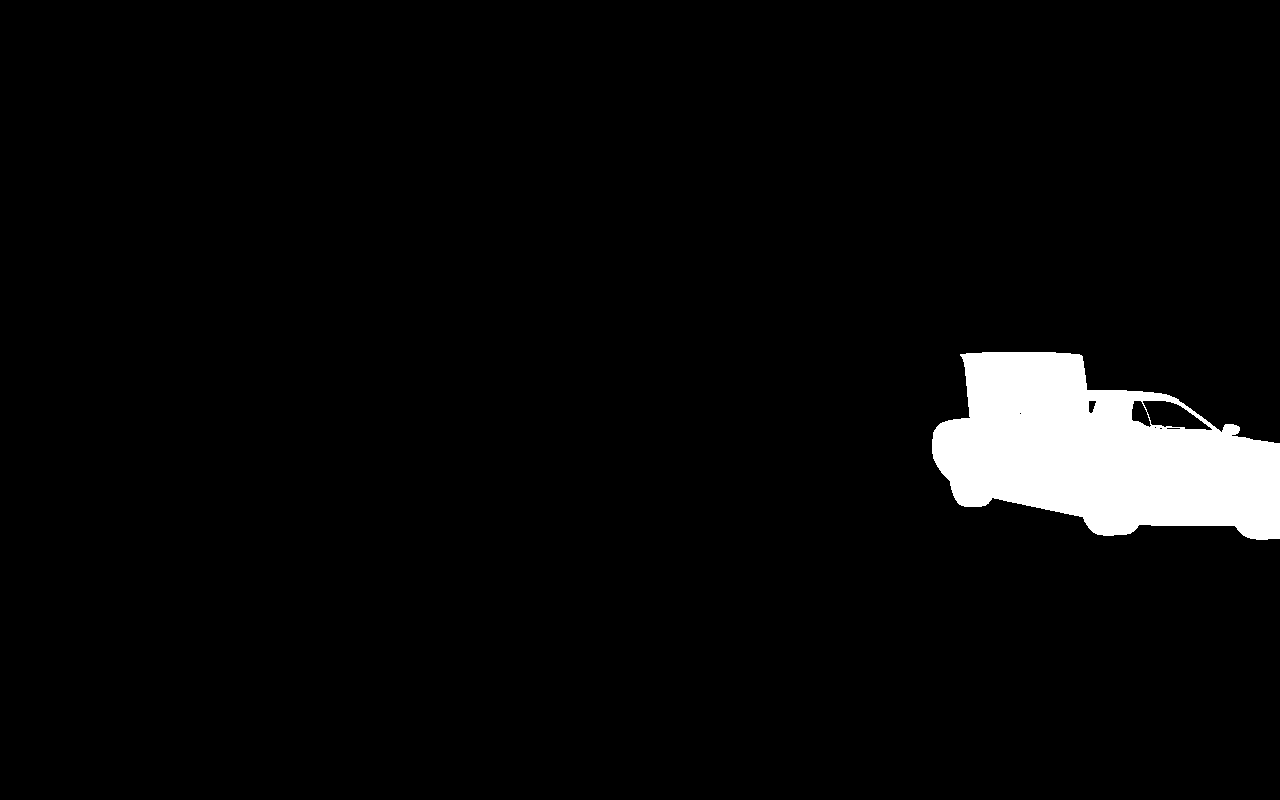
\includegraphics[scale=0.07]{good_examples/visual_29224_gt.png}
\end{subfigure}
\begin{subfigure}[t]{0.19\textwidth}
\centering
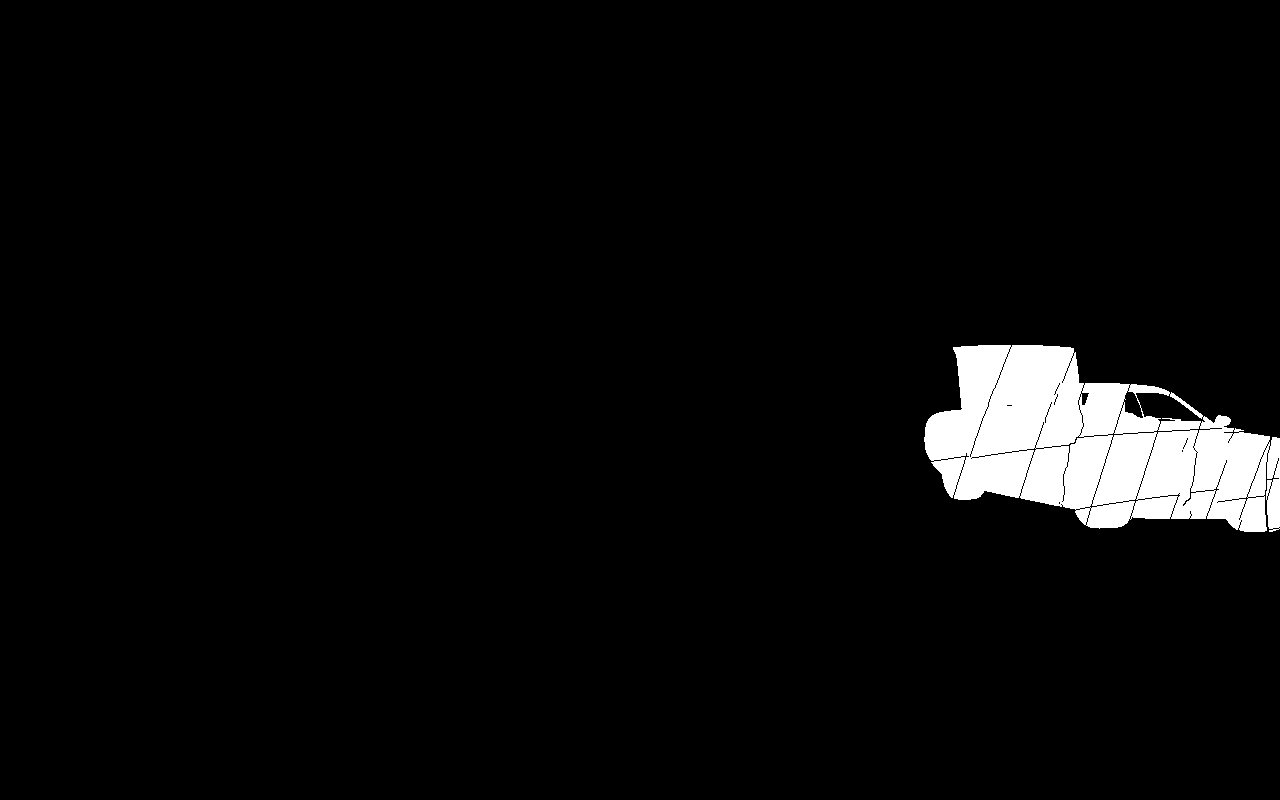
\includegraphics[scale=0.07]{good_examples/visual_29224_w_np.png}
\end{subfigure}
\begin{subfigure}[t]{0.19\textwidth}
\centering
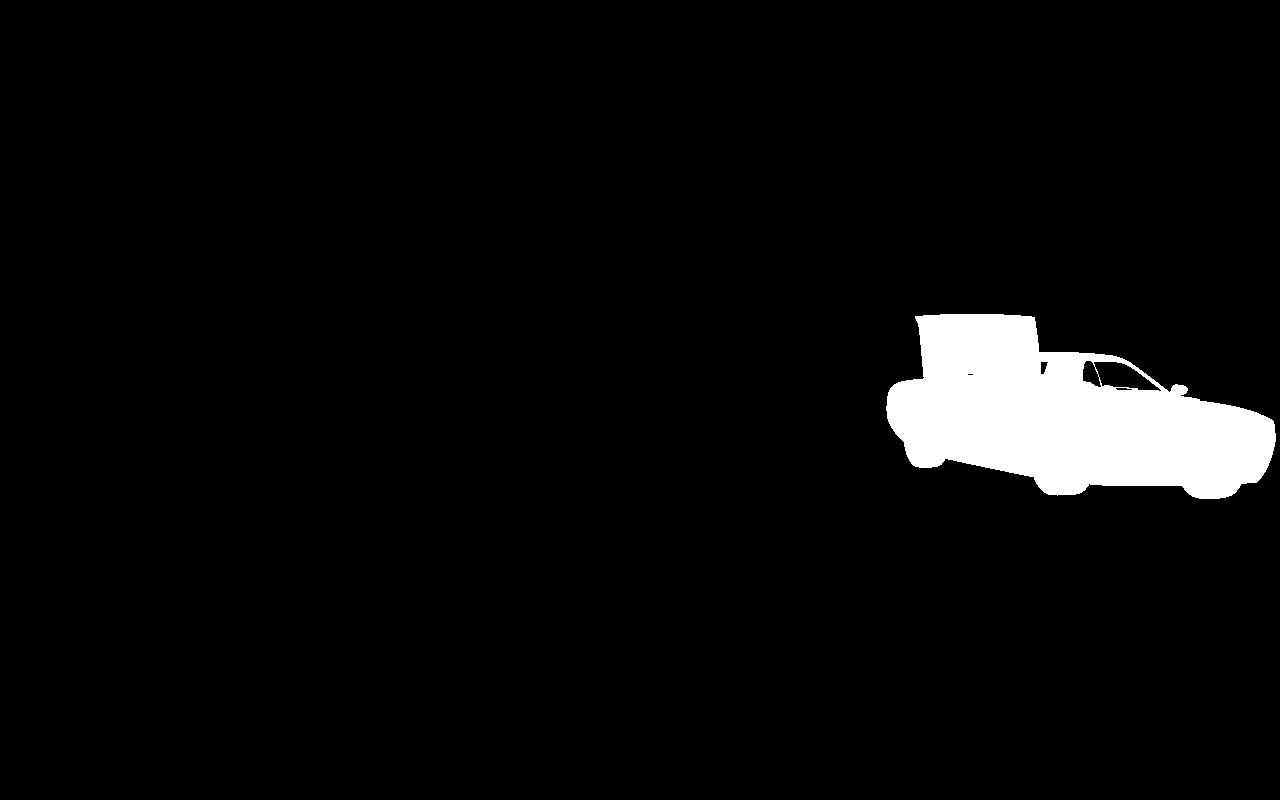
\includegraphics[scale=0.07]{good_examples/visual_29224_wo_np.png}
\end{subfigure}
\caption{IOU with reprojection: 0.82, IOU without reprojection: 0.51, video\_name: bs\_2a\_mcs\_8, frame\_number: 498.}
\end{figure}

\begin{figure}
\centering
\begin{subfigure}[t]{0.19\textwidth}
\centering
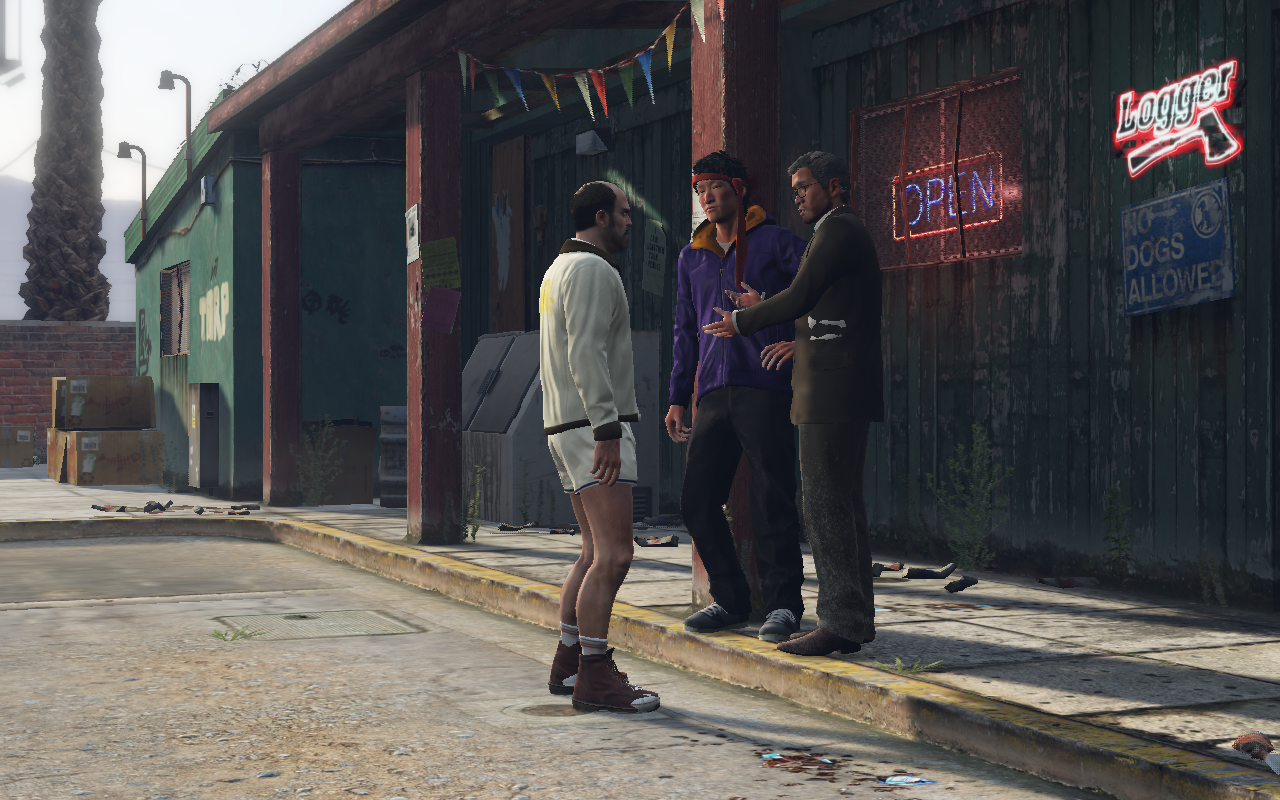
\includegraphics[scale=0.07]{good_examples/visual_81815_img.png}
\end{subfigure}
\begin{subfigure}[t]{0.19\textwidth}
\centering
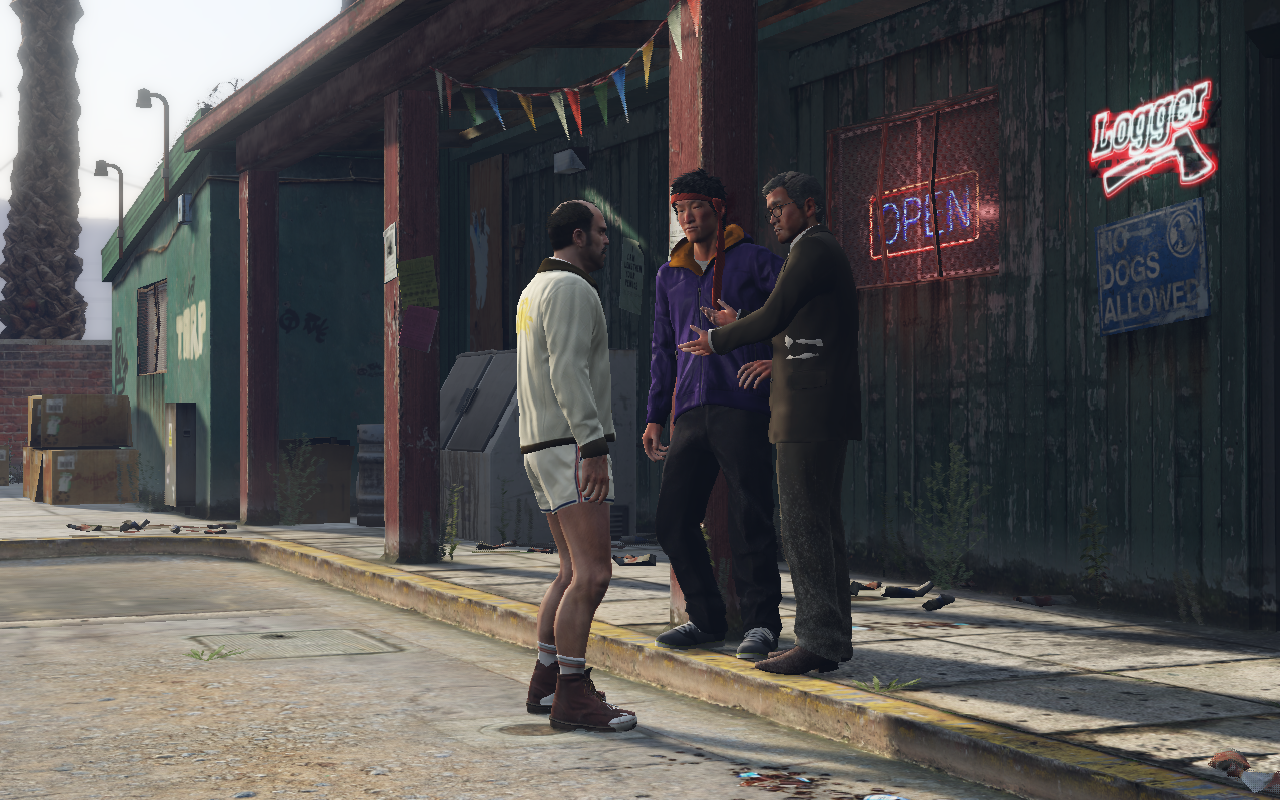
\includegraphics[scale=0.07]{good_examples/visual_81815_img1.png}
\end{subfigure}
\begin{subfigure}[t]{0.19\textwidth}
\centering

\includegraphics[scale=0.07]{good_examples/visual_81815_gt.png}
\end{subfigure}
\begin{subfigure}[t]{0.19\textwidth}
\centering
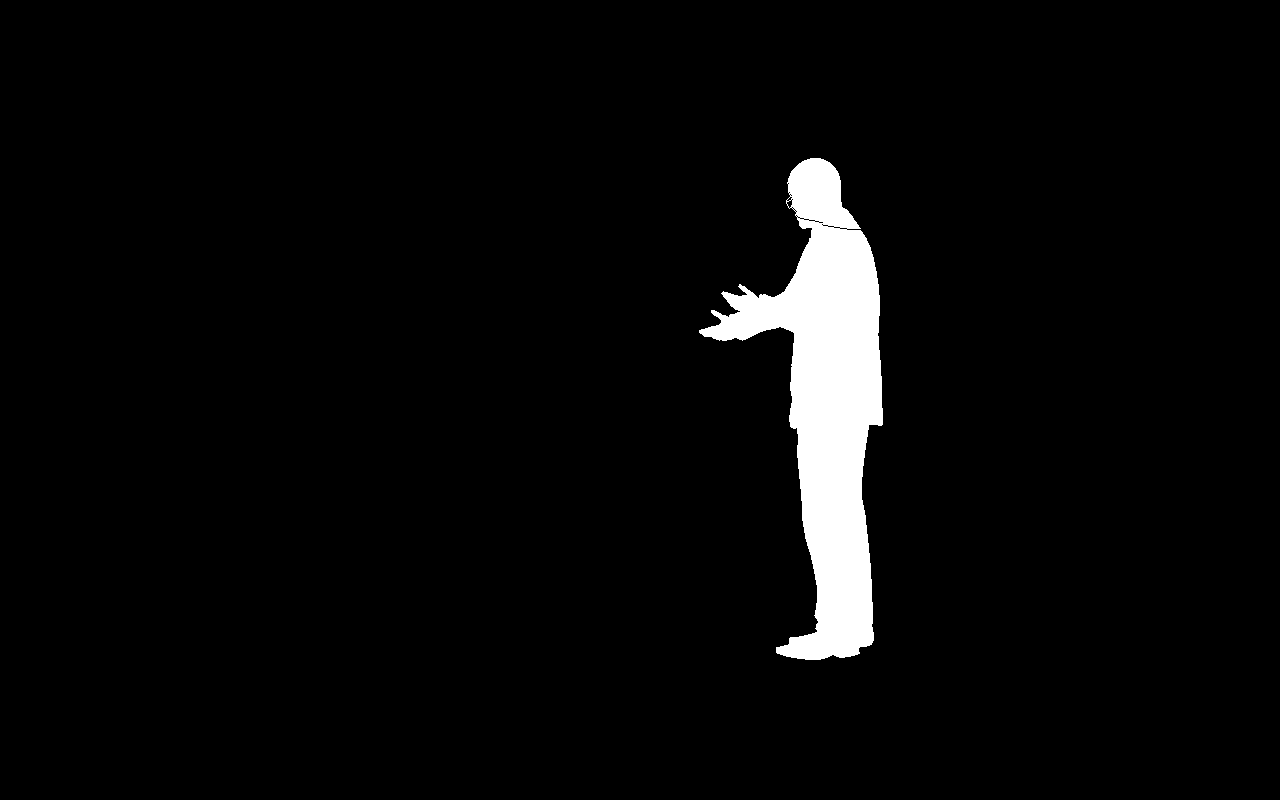
\includegraphics[scale=0.07]{good_examples/visual_81815_w_np.png}
\end{subfigure}
\begin{subfigure}[t]{0.19\textwidth}
\centering
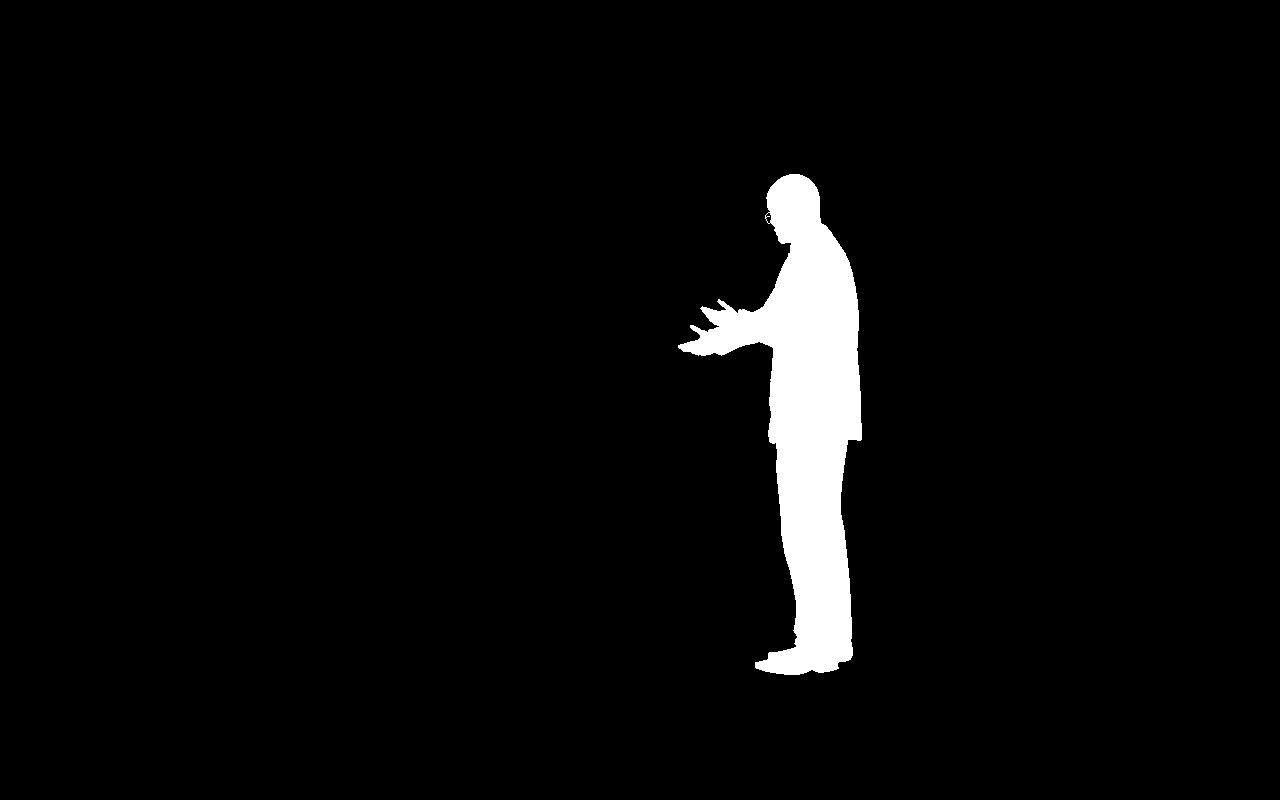
\includegraphics[scale=0.07]{good_examples/visual_81815_wo_np.png}
\end{subfigure}
\caption{IOU with reprojection: 0.90, IOU without reprojection: 0.47, video\_name: chinese\_2\_int, frame\_number: 456.}
\end{figure}

\begin{figure}
\centering
\begin{subfigure}[t]{0.19\textwidth}
\centering
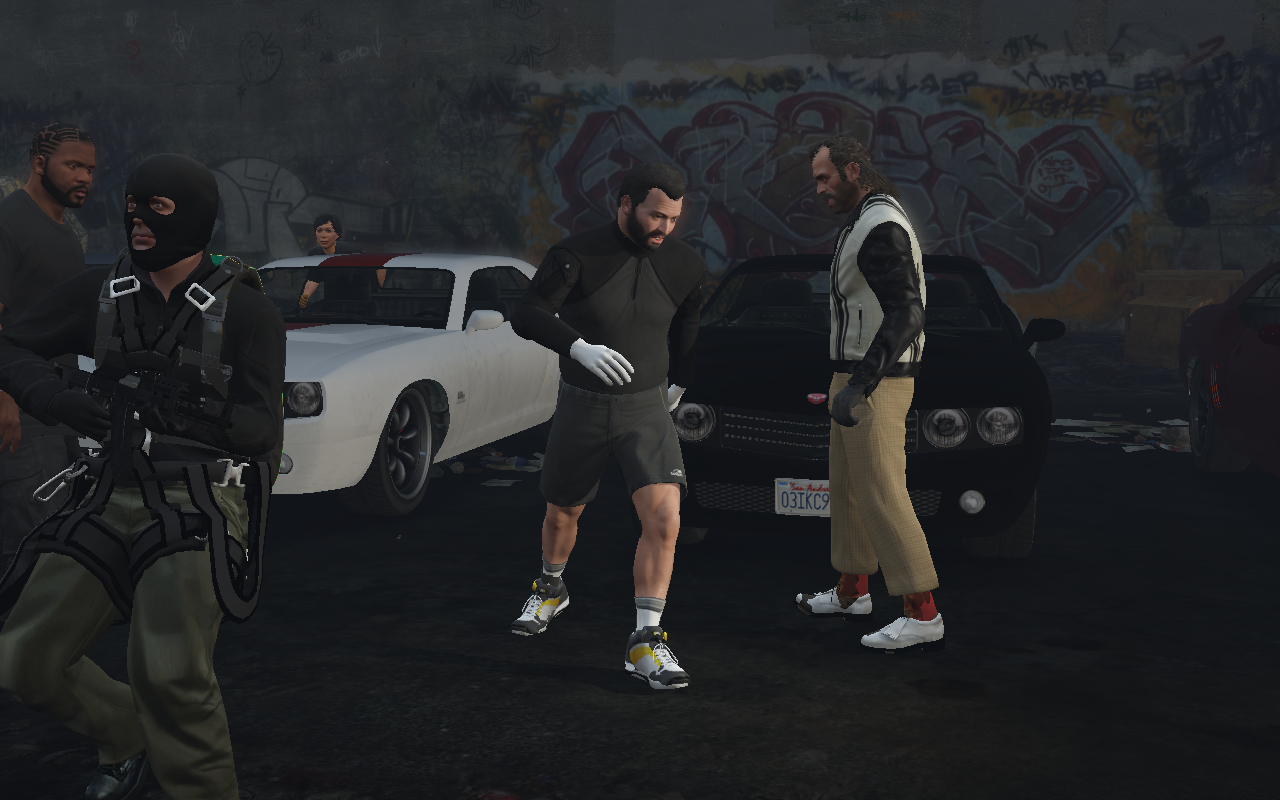
\includegraphics[scale=0.07]{good_examples/visual_34430_img.png}
\end{subfigure}
\begin{subfigure}[t]{0.19\textwidth}
\centering
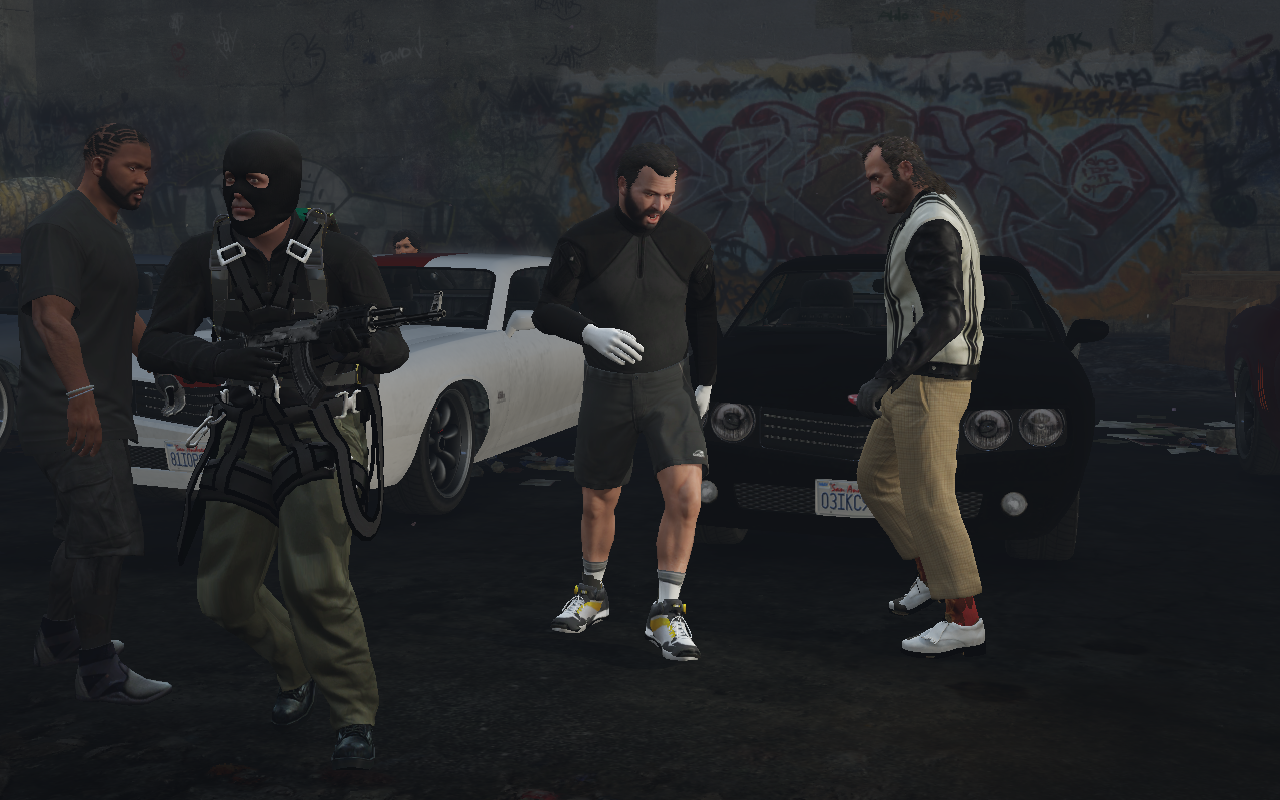
\includegraphics[scale=0.07]{good_examples/visual_34430_img1.png}
\end{subfigure}
\begin{subfigure}[t]{0.19\textwidth}
\centering
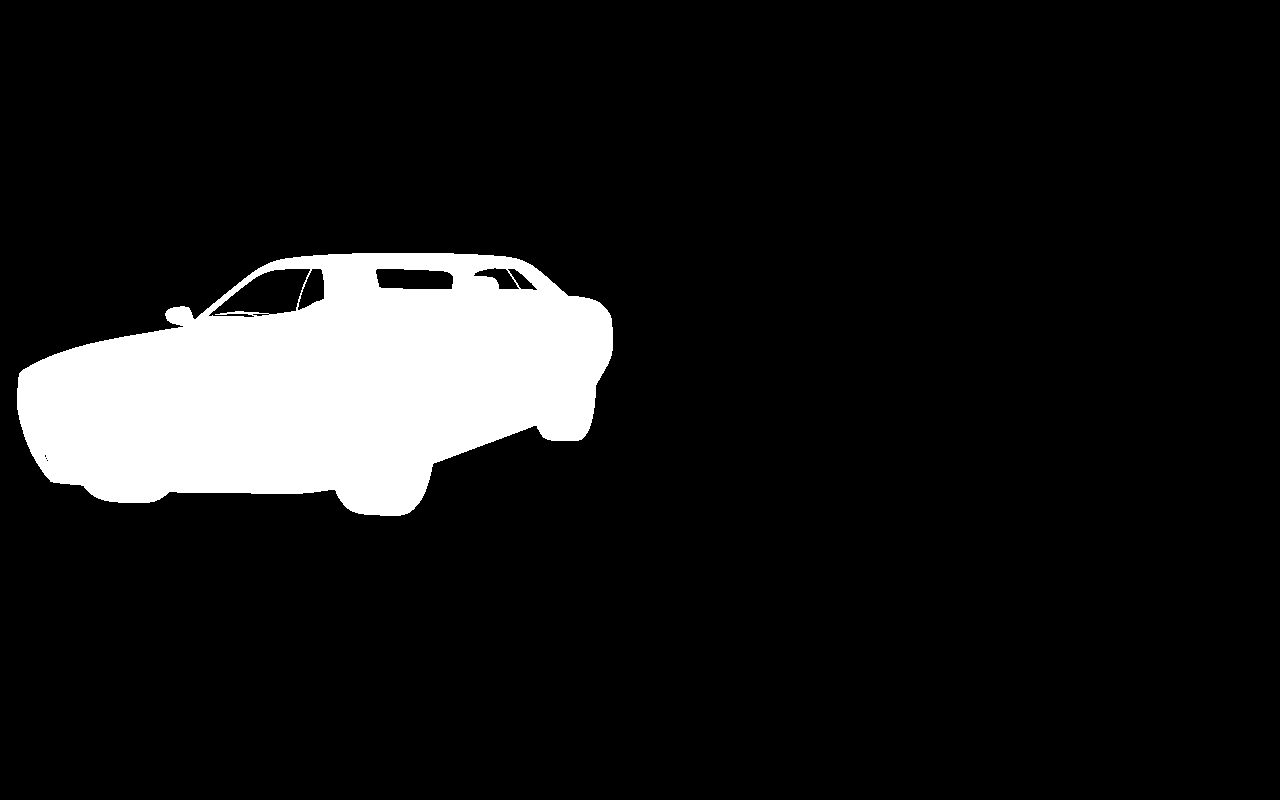
\includegraphics[scale=0.07]{good_examples/visual_34430_gt.png}
\end{subfigure}
\begin{subfigure}[t]{0.19\textwidth}
\centering
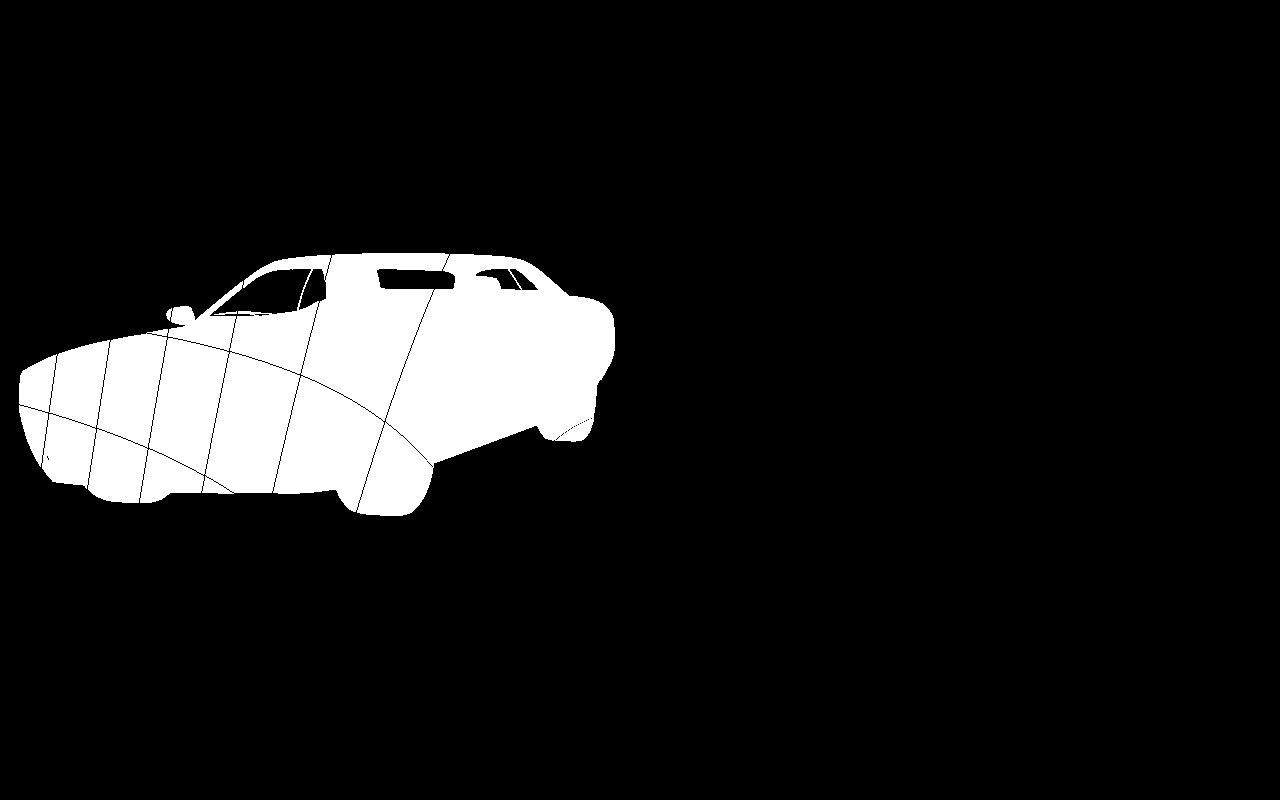
\includegraphics[scale=0.07]{good_examples/visual_34430_w_np.png}
\end{subfigure}
\begin{subfigure}[t]{0.19\textwidth}
\centering
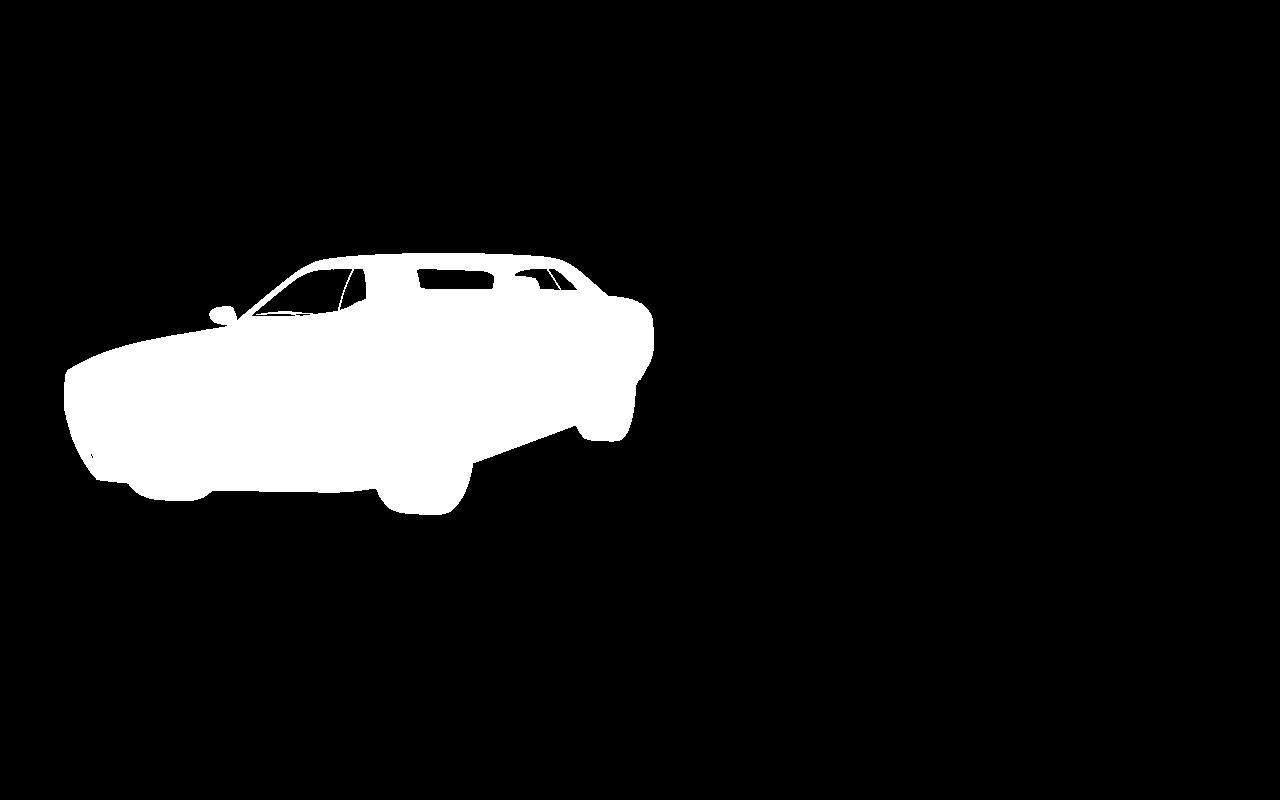
\includegraphics[scale=0.07]{good_examples/visual_34430_wo_np.png}
\end{subfigure}
\caption{IOU with reprojection: 0.97, IOU without reprojection: 0.76, video\_name: bs\_2a\_mcs\_8\_p3, frame\_number: 79.}
\end{figure}

\begin{figure}
\centering
\begin{subfigure}[t]{0.19\textwidth}
\centering
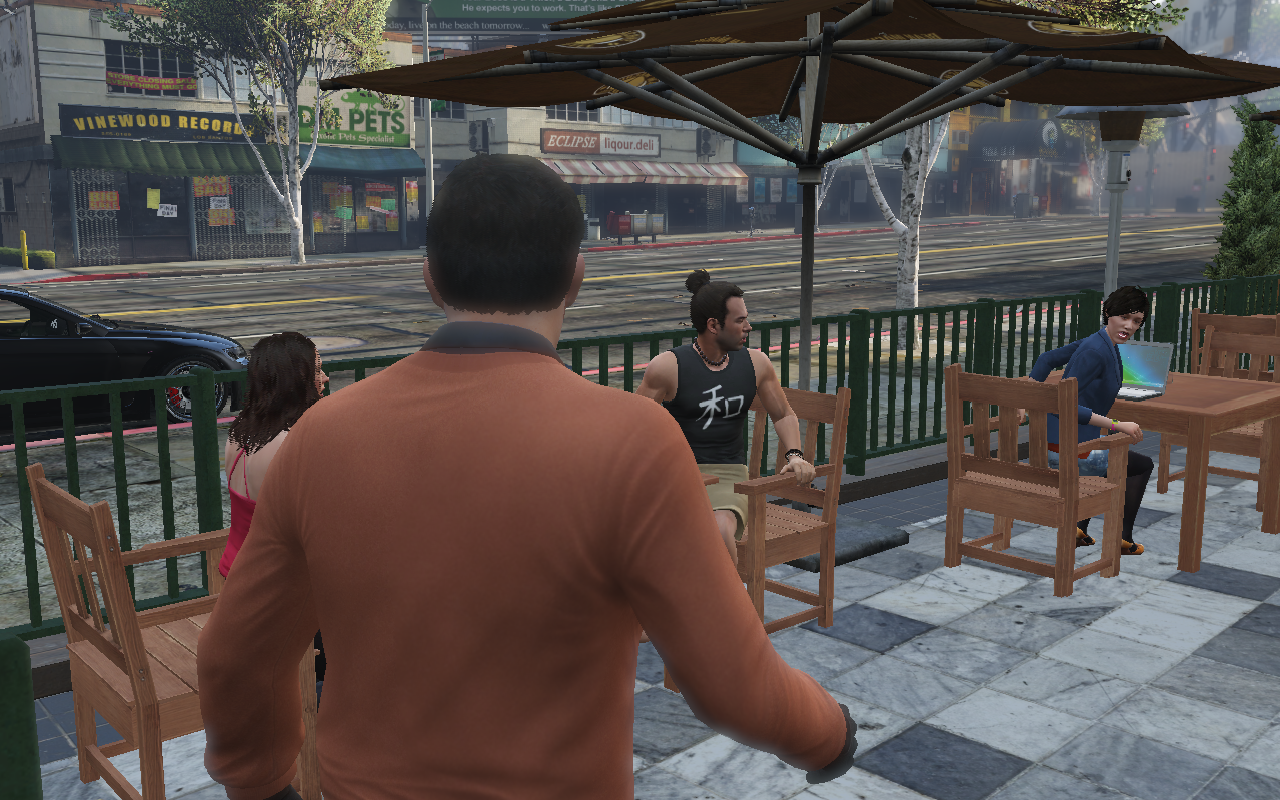
\includegraphics[scale=0.07]{good_examples/visual_99358_img.png}
\end{subfigure}
\begin{subfigure}[t]{0.19\textwidth}
\centering
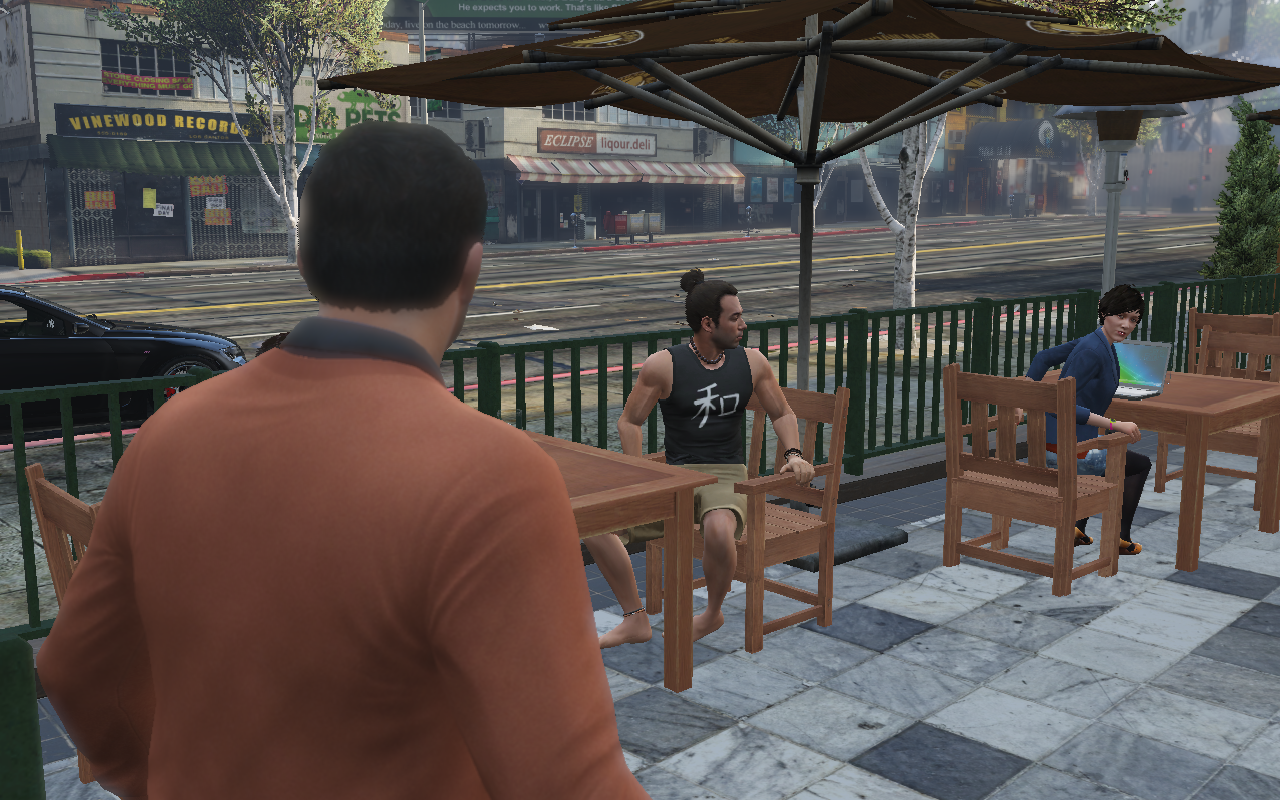
\includegraphics[scale=0.07]{good_examples/visual_99358_img1.png}
\end{subfigure}
\begin{subfigure}[t]{0.19\textwidth}
\centering
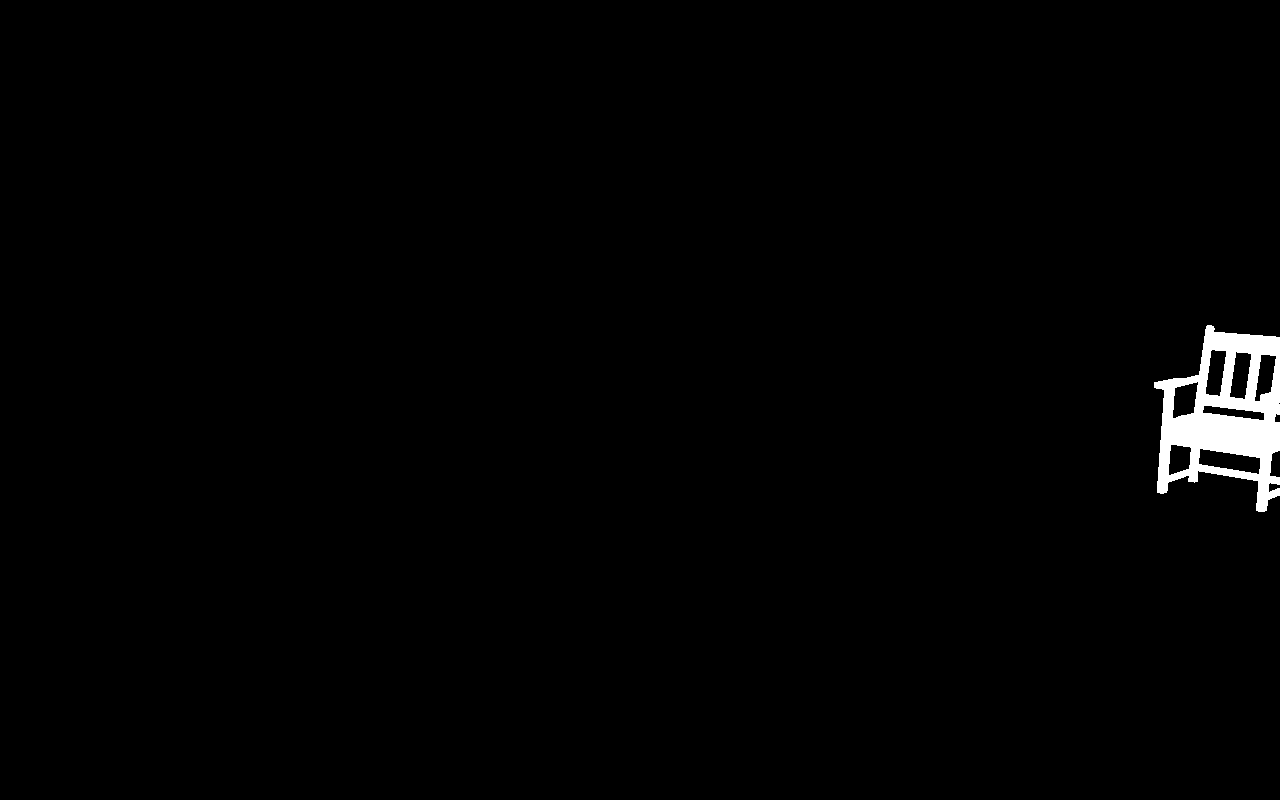
\includegraphics[scale=0.07]{good_examples/visual_99358_gt.png}
\end{subfigure}
\begin{subfigure}[t]{0.19\textwidth}
\centering
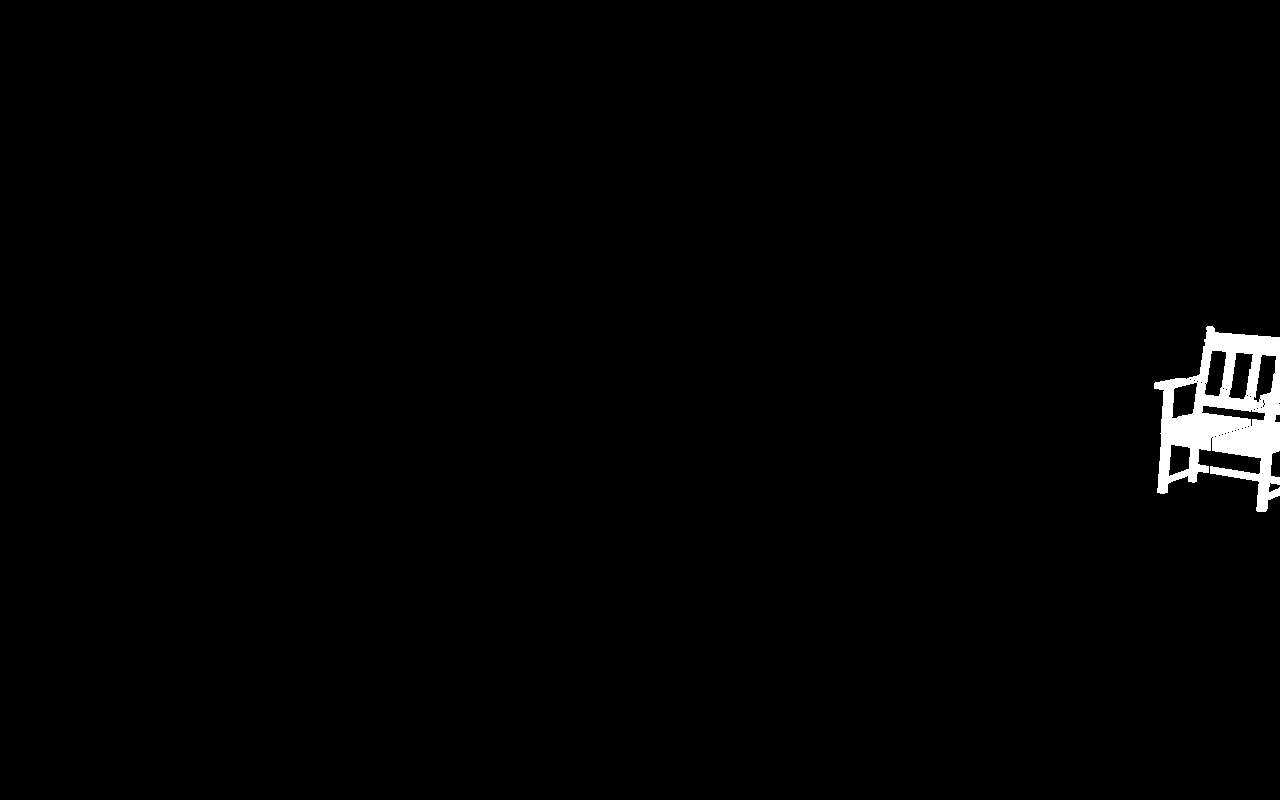
\includegraphics[scale=0.07]{good_examples/visual_99358_w_np.png}
\end{subfigure}
\begin{subfigure}[t]{0.19\textwidth}
\centering
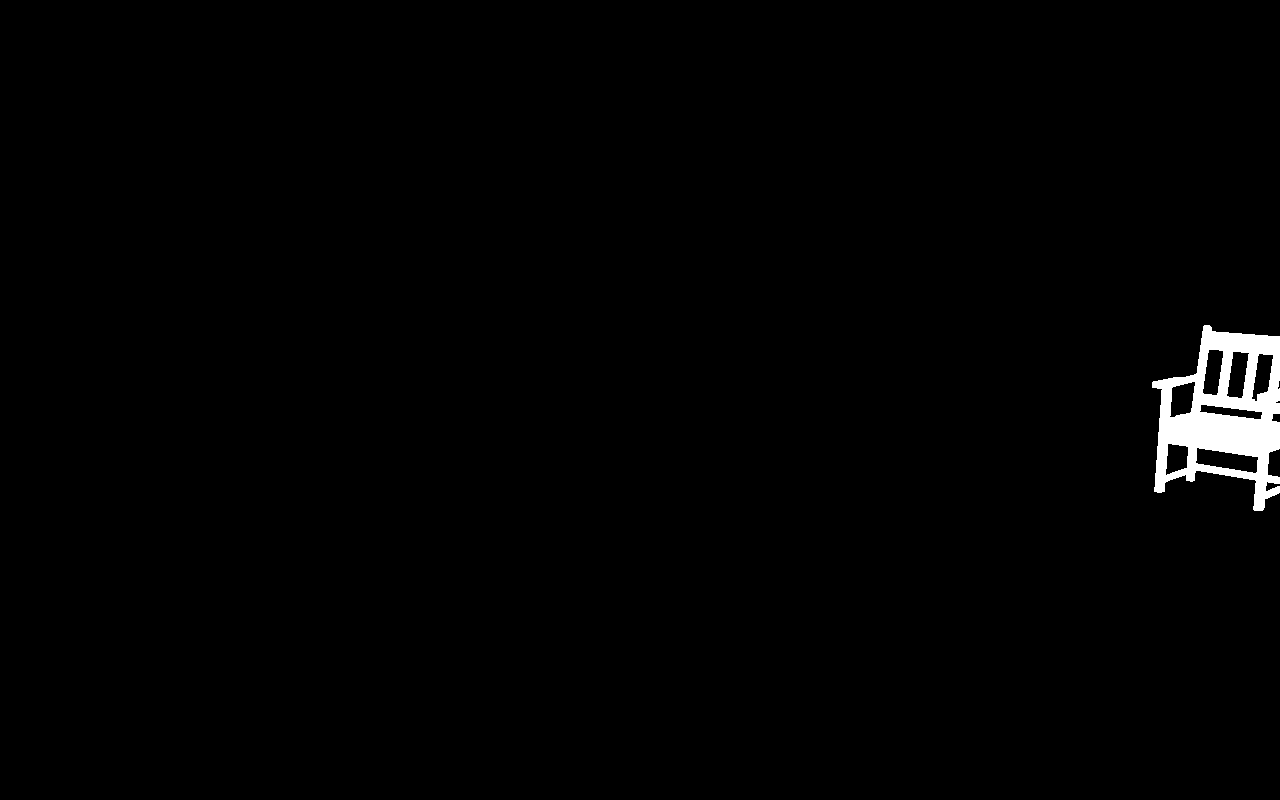
\includegraphics[scale=0.07]{good_examples/visual_99358_wo_np.png}
\end{subfigure}
\caption{IOU with reprojection: 0.94, IOU without reprojection: 0.81, video\_name: fam\_6\_mcs\_1, frame\_number: 25.}
\end{figure}

\begin{figure}
\centering
\begin{subfigure}[t]{0.19\textwidth}
\centering
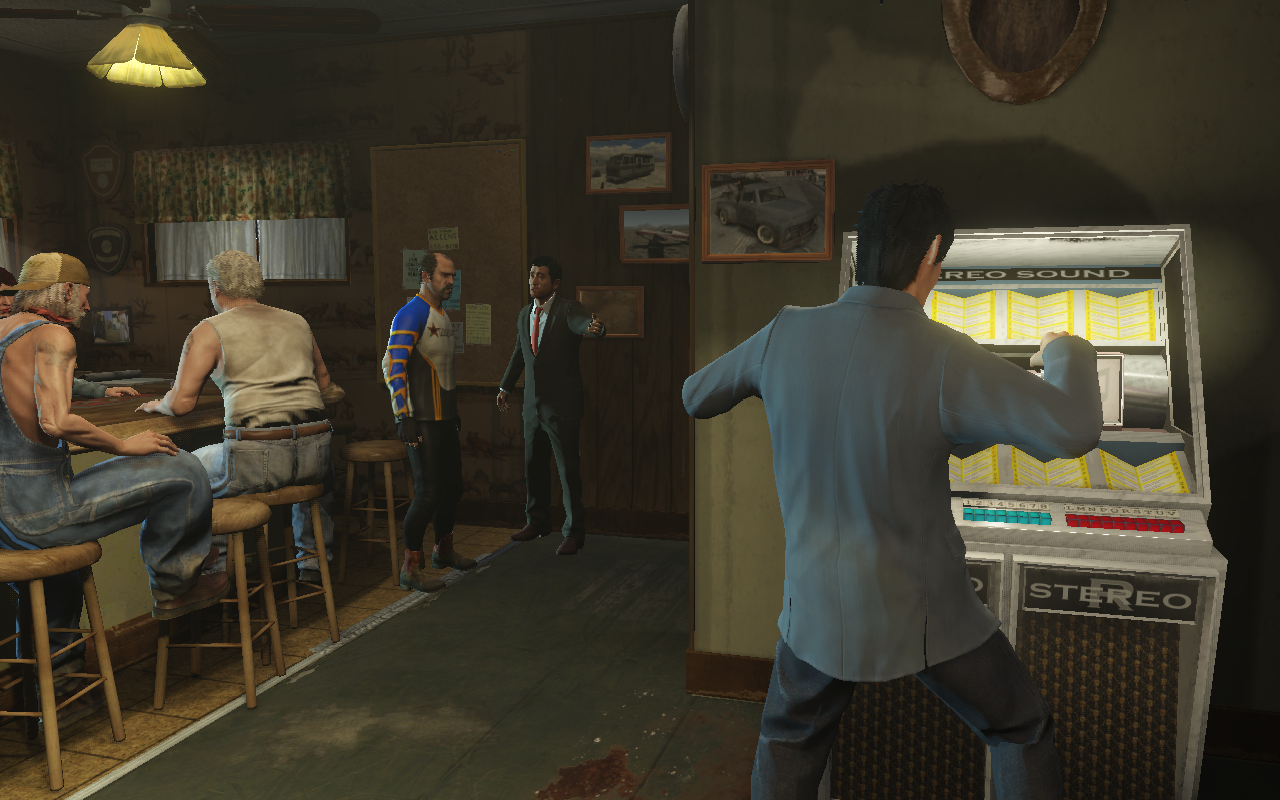
\includegraphics[scale=0.07]{good_examples/visual_69756_img.png}
\end{subfigure}
\begin{subfigure}[t]{0.19\textwidth}
\centering
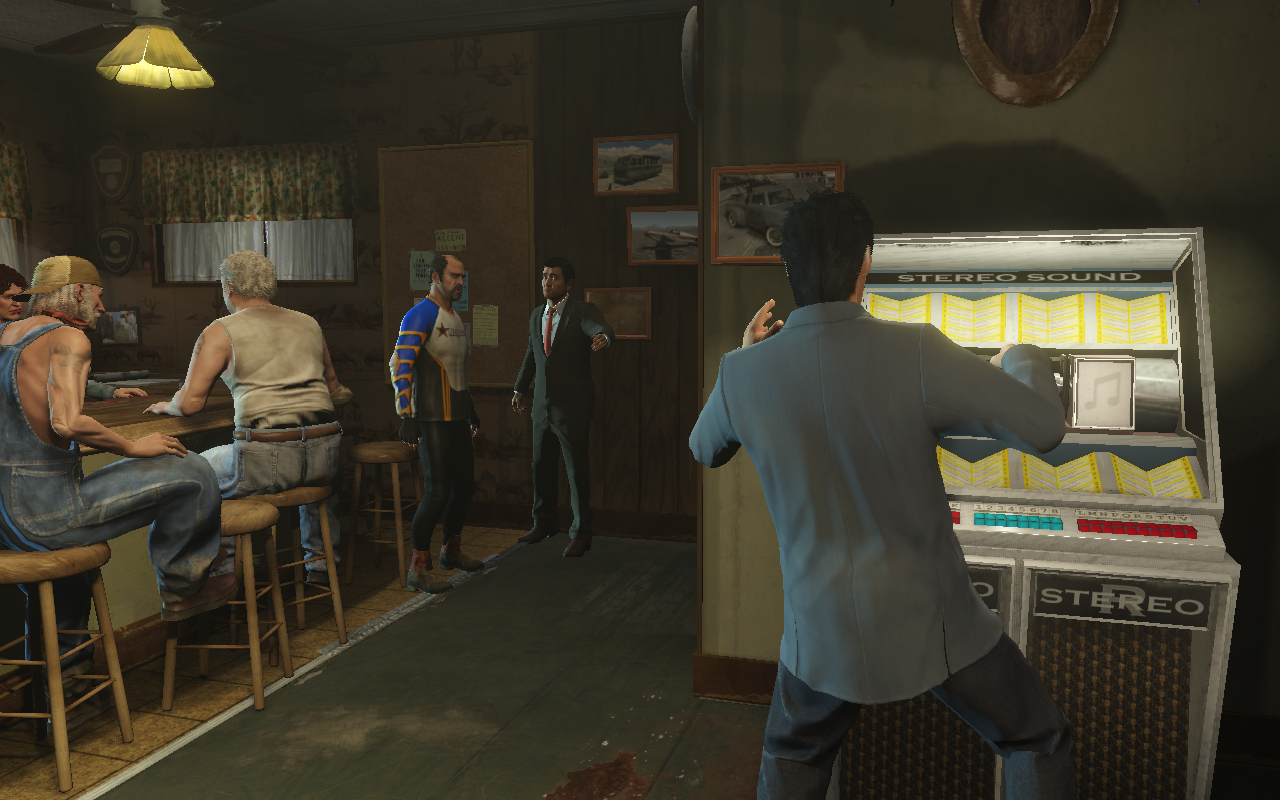
\includegraphics[scale=0.07]{good_examples/visual_69756_img1.png}
\end{subfigure}
\begin{subfigure}[t]{0.19\textwidth}
\centering
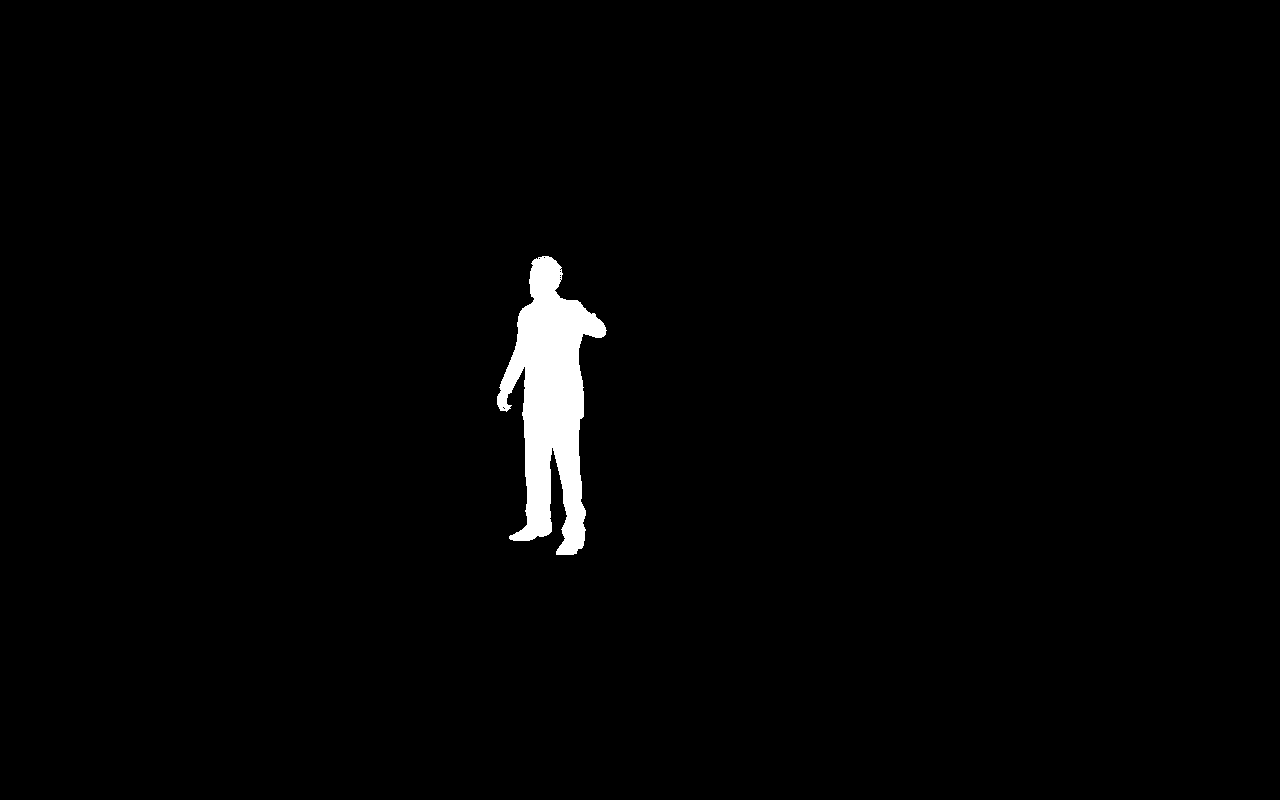
\includegraphics[scale=0.07]{good_examples/visual_69756_gt.png}
\end{subfigure}
\begin{subfigure}[t]{0.19\textwidth}
\centering
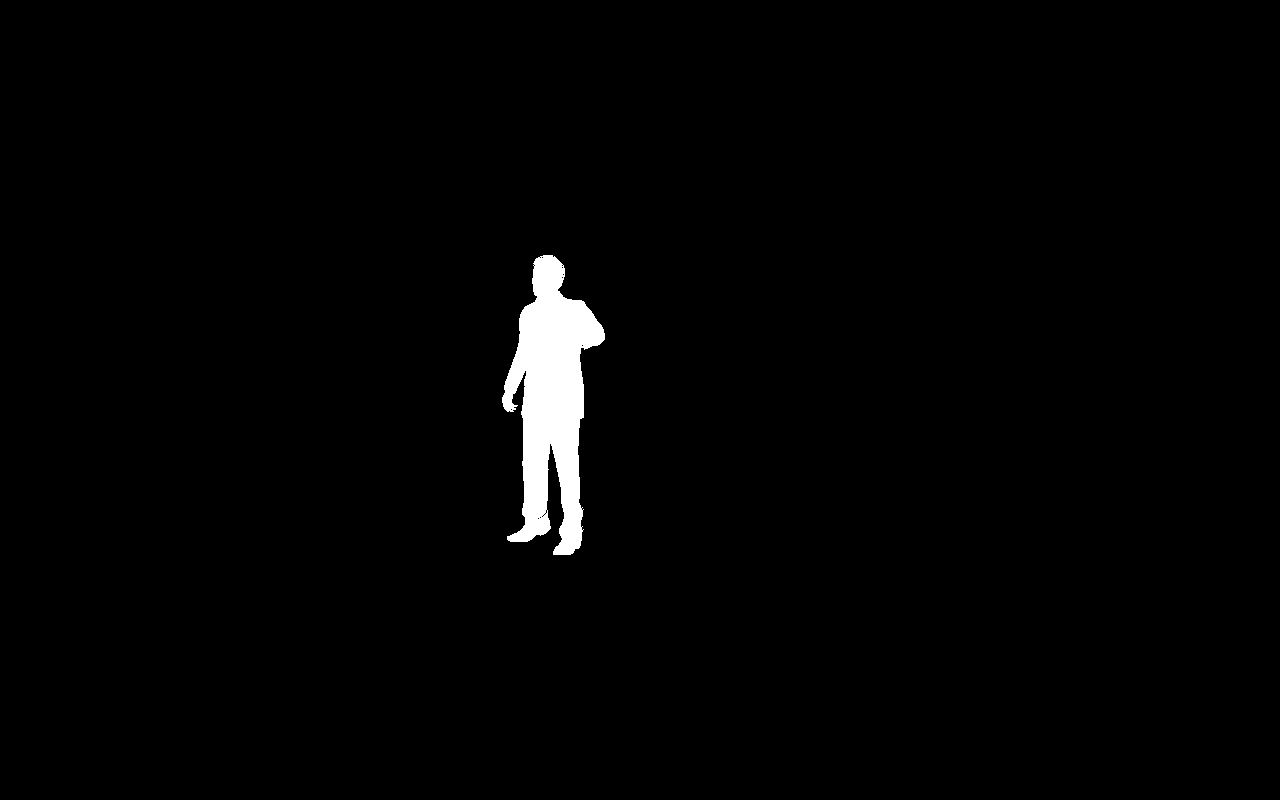
\includegraphics[scale=0.07]{good_examples/visual_69756_w_np.png}
\end{subfigure}
\begin{subfigure}[t]{0.19\textwidth}
\centering
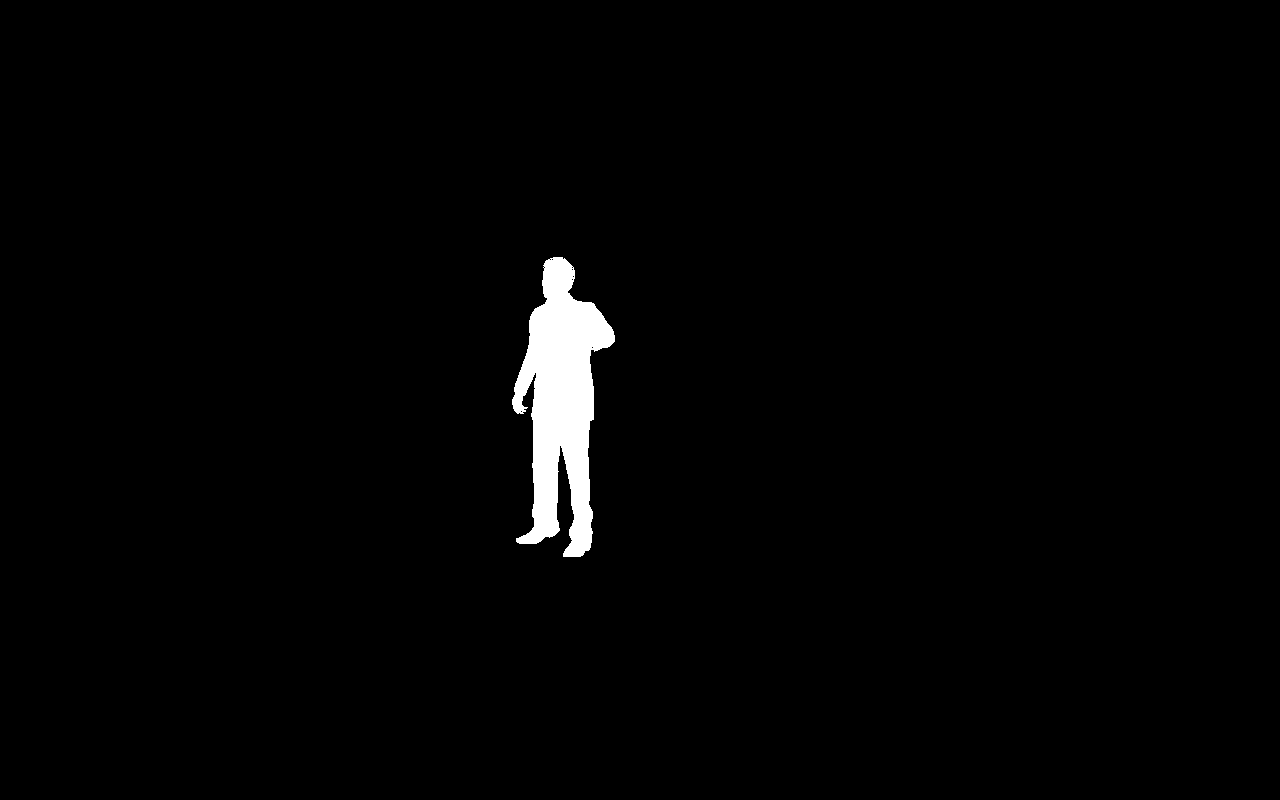
\includegraphics[scale=0.07]{good_examples/visual_69756_wo_np.png}
\end{subfigure}
\caption{IOU with reprojection: 0.87, IOU without reprojection: 0.59, video\_name: chinese\_1\_int, frame\_number: 550.}
\end{figure}




\begin{figure}
\centering
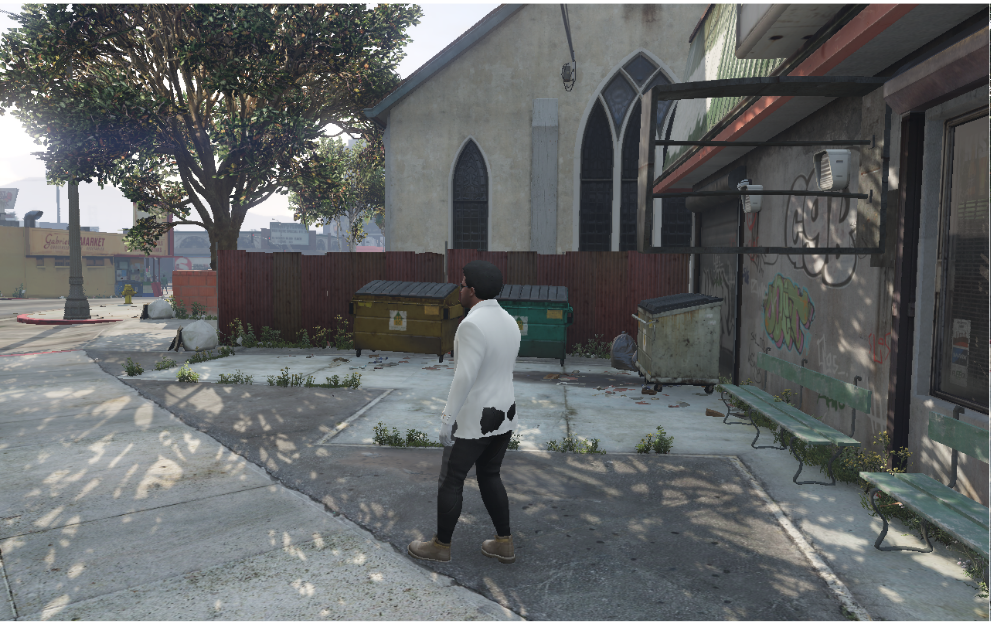
\includegraphics[scale=0.2]{fig/270i.png}
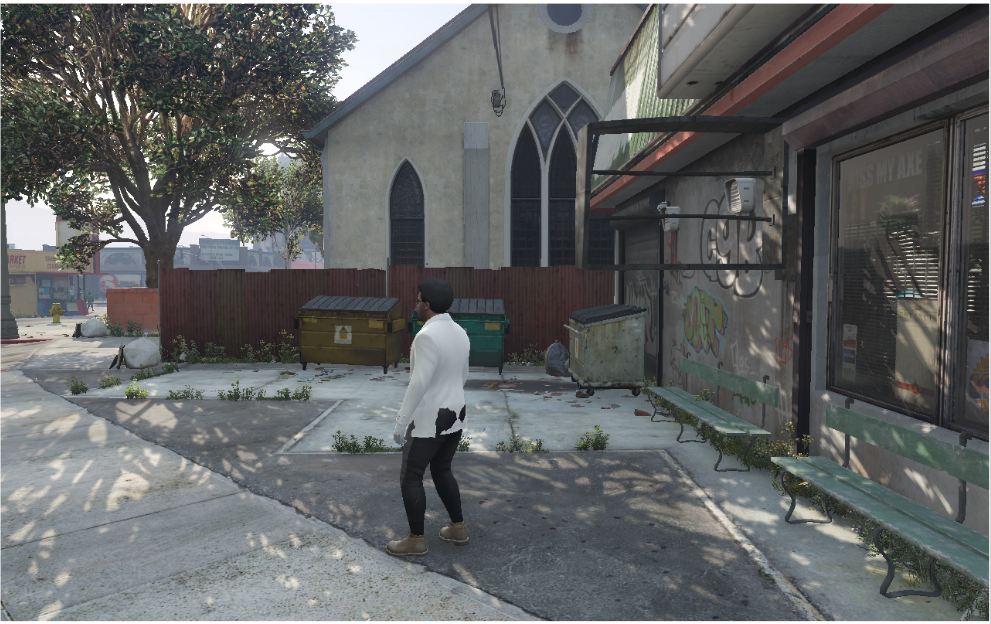
\includegraphics[scale=0.2]{fig/271i.png}
\includegraphics[scale=0.38]{fig/270r271.png}
\caption{Image from SAILVOS dataset video \text{tonya\_concat\_1} frame 270 and 271. The third figure is the result of reproject frame 270 to the view of 271. We can see that the camera moved left from frame 270 to 271, which is reflected in the reprojected image.}
\label{fig:reproj_image}
\end{figure}

\section{Implementation Details}
%Our implementation follows the same set of hyperparameters in~\cite{he2017mask} based on the implementation in Detectron2~\cite{wu2019detectron2}. %\as{doesn't this sentence diminish; formulate better}   More specifically, we use the setup of
We use
ResNet50~\cite{he2016deep} with FPN~\cite{lin2017feature} backbone for all experiments. 
For initialization, we use the COCO pre-trained weights with the standard $1\times$ training schedule. 

All layers introduced in our approach are randomly initialized following Kaiming initialization~\cite{he2015delving}.  %and train them on the corresponding Amodal dataset using SGD with momentum. 
%
All models are trained using SGD with momentum and a default data-augmentation from Detectron2~\cite{wu2019detectron2}, which includes random horizontal flipping and re-sizing of the images. We extract optical flow using LiteFlowNet2~\cite{hui2020lightweight}.
For Soft-NMS~\cite{bodla2017soft}, we use the linear weighting scheme for all the cascaded box iterations during training. At test-time, we use a test-threshold of $0.3$ for all stages of the box prediction.


\chapter{Experiments}
\label{chp:exp}
%!TEX root = main.tex

\begin{figure*}[t]
    \centering
    \setlength{\tabcolsep}{1pt}
    %\renewcommand{\arraystretch}{0.5}
    \renewcommand{\arraystretch}{4.3}
    \begin{tabular}{ccccc}
    % GT
    GT & 
    \includegraphics[align=c,width=0.23\linewidth]{fig/sailvos_results/21781_gt} &
    \includegraphics[align=c,width=0.23\linewidth]{fig/sailvos_results/10561_gt} &
    \includegraphics[align=c,width=0.23\linewidth]{fig/sailvos_results/14498_gt} &
    %\includegraphics[align=c,width=0.23\linewidth]{fig/sailvos_results/11413_gt} &
    \includegraphics[align=c,width=0.23\linewidth]{fig/sailvos_results/22243_gt}
    \\
    % Baseline 
    \cite{hu2019sail} & 
    \includegraphics[align=c,width=0.23\linewidth]{fig/sailvos_results/21781_base} &
    \includegraphics[align=c,width=0.23\linewidth]{fig/sailvos_results/10561_base} &
    \includegraphics[align=c,width=0.23\linewidth]{fig/sailvos_results/14498_base} &
    %\includegraphics[align=c,width=0.23\linewidth]{fig/sailvos_results/11413_base} &
    \includegraphics[align=c,width=0.23\linewidth]{fig/sailvos_results/22243_base}
    \\
    % Ours
    Ours &
    \includegraphics[align=c,width=0.23\linewidth]{fig/sailvos_results/21781_ours} &
    \includegraphics[align=c,width=0.23\linewidth]{fig/sailvos_results/10561_ours} &
    \includegraphics[align=c,width=0.23\linewidth]{fig/sailvos_results/14498_ours} &
    %\includegraphics[align=c,width=0.23\linewidth]{fig/sailvos_results/11413_ours} &
    \includegraphics[align=c,width=0.23\linewidth]{fig/sailvos_results/22243_ours}
    \end{tabular}
    \vspace{-0.25cm}
    \caption{Qualitative comparison with~\cite{hu2019sail} on SAIL-VOS dataset in the class-specific setting.
    %\as{using the class-specific setting?}.
    }
    \label{fig:qual_result}
    \vspace{-0.25cm}
    \end{figure*}
    
    
    
    %\begin{tabular}{ccccc}
    %% GT
    %GT & 
    %\includegraphics[align=c,width=0.23\linewidth]{fig/sailvos_results/14498_gt} &
    %\includegraphics[align=c,width=0.23\linewidth]{fig/sailvos_results/21781_gt} &
    %\includegraphics[align=c,width=0.23\linewidth]{fig/sailvos_results/10561_gt} &
    %%\includegraphics[align=c,width=0.23\linewidth]{fig/sailvos_results/11413_gt} &
    %\includegraphics[align=c,width=0.23\linewidth]{fig/sailvos_results/22243_gt}
    %\\
    %% Baseline 
    %\cite{hu2019sail} & 
    %\includegraphics[align=c,width=0.23\linewidth]{fig/sailvos_results/14498_base} &
    %\includegraphics[align=c,width=0.23\linewidth]{fig/sailvos_results/21781_base} &
    %\includegraphics[align=c,width=0.23\linewidth]{fig/sailvos_results/10561_base} &
    %%\includegraphics[align=c,width=0.23\linewidth]{fig/sailvos_results/11413_base} &
    %\includegraphics[align=c,width=0.23\linewidth]{fig/sailvos_results/22243_base}
    %\\
    %% Ours
    %Ours &
    %\includegraphics[align=c,width=0.23\linewidth]{fig/sailvos_results/14498_ours} &
    %\includegraphics[align=c,width=0.23\linewidth]{fig/sailvos_results/21781_ours} &
    %\includegraphics[align=c,width=0.23\linewidth]{fig/sailvos_results/10561_ours} &
    %%\includegraphics[align=c,width=0.23\linewidth]{fig/sailvos_results/11413_ours} &
    %\includegraphics[align=c,width=0.23\linewidth]{fig/sailvos_results/22243_ours}
    %\end{tabular}
    
    %\begin{tabular}{ccc}
    %\includegraphics[width=0.31\linewidth]{fig/sailvos_results/14498_gt} & \includegraphics[width=0.31\linewidth]{fig/sailvos_results/14498_base} & \includegraphics[width=0.31\linewidth]{fig/sailvos_results/14498_ours}\\
    %\includegraphics[width=0.31\linewidth]{fig/sailvos_results/21781_gt} &
    %\includegraphics[width=0.31\linewidth]{fig/sailvos_results/21781_base} &
    %\includegraphics[width=0.31\linewidth]{fig/sailvos_results/21781_ours}\\
    %\includegraphics[width=0.31\linewidth]{fig/sailvos_results/11413_gt} & 
    %\includegraphics[width=0.31\linewidth]{fig/sailvos_results/11413_base} & 
    %\includegraphics[width=0.31\linewidth]{fig/sailvos_results/11413_ours}\\
    %GT & MaskJoint & Ours
    %\end{tabular}
    
    %\begin{figure*}[t]
    %{
    %\centering
    %\includegraphics[width=0.99\textwidth]{fig/sailvos_results/21781}
    %\includegraphics[width=0.99\textwidth]{fig/sailvos_results/14498}\\
    %}
    %\hspace{2.9cm}Ground-Truth  \hspace{2.8cm} MaskJoint~\cite{hu2019sail}  \hspace{3.2cm} Oursz
    %\caption{Qualitative comparisons with~\cite{hu2019sail} on SAILVOS dataset. 
    %}
    %\label{fig:qual_result}
    %\end{figure*}
    
%!TEX root = ../main.tex
\begin{table*}[t]
\centering
\renewcommand{\arraystretch}{0.95}
\begin{tabular*}{\textwidth}{@{\extracolsep{\fill}}c|ccccccccc}
\specialrule{.15em}{.05em}{.05em}
Row \# & Method &  Occlude & Flow & \# Mask Layers & Cascade & Soft-NMS & Mask Iter. & Box AP & Mask AP\\
\hline\hline
%MaskAmodal~\cite{follmann2019learning} & \xmark & \xmark & 4 & \xmark & \xmark & \xmark & - & 13.0\\ 
%MaskJoint~\cite{hu2019sail} & \xmark & \xmark & 4 & \xmark & \xmark & \xmark & - & 14.1\\
1 & MaskJoint~\cite{hu2019sail} & \xmark&  \xmark & 4 & \xmark & \xmark  & \xmark & - & 14.1\\
2 & Ours & \cmark & \xmark & 4 & \xmark & \xmark  & \xmark & 16.4 & 14.6\\
\hline 
3 & Ours & \cmark & \xmark & 9 &\xmark  & \xmark & \xmark & 16.4  & 15.4\\
4 & Ours & \cmark & \xmark & 10 &\xmark  & \xmark & \xmark &  16.4 & 15.3\\
\hline
5 & Ours & \cmark & \cmark & 9 &\xmark  & \xmark & \xmark &  17.5 & 16.3 \\
\hline 
6 & Ours & \cmark & \cmark & 9 &\cmark  & \xmark & \xmark &  18.6 & 16.7 \\
7 & Ours & \cmark & \cmark & 9 &\cmark  & \cmark & \xmark &   19.6 & 17.3\\
8 & Ours & \cmark & \cmark & 9 &\cmark  & \cmark & \cmark &  \bf 19.6 & \bf 17.6\\
%\cite{hu2019sail} & \xmark & \xmark & - & 13.0 & - & -\\

%\hline
%Ours & \xmark & \xmark &  16.24 & 14.15 & - & - \\
%Ours & \cmark & \cmark &   16.40 & 14.58 & 14.47 & 1.502\\
%\hline
%Ours+6conv. & \xmark & \xmark &  16.26 & 14.90 & - & -\\
%Ours+6conv. & \cmark & \cmark & 16.40  & 15.39 & 14.98 & 2.002\\
%Ours+5conv. & \cmark & \cmark & 16.40  & 15.39 & 14.98 & 2.002\\
%\hline
%Ours+5conv.+flow+soft\_nms & \cmark & \cmark & \bf 17.47 & \bf 16.25 & \bf 15.82 & \bf 2.079\\
\specialrule{.15em}{.05em}{.05em}
\end{tabular*}
\vspace{-0.3cm}
\caption{Ablation study for each of the proposed components on the SAIL-VOS dataset using the class-specific setting.}
\label{tab:abalation}
\vspace{-0.5cm}
\end{table*}



\section{Metrics and Baseline}

To evaluate amodal segmentation, we report the commonly used average precision (AP) averaged over IoU thresholds from $50\%$ to $95\%$. We also report AP with an IoU threshold of 50\%, \ie, $\text{AP}_{50}$. To further study the results, we compute a range of metrics, including $\text{AP}_{\text{50}}^{\text{P}}$ and  $\text{AP}_{\text{50}}^{\text{H}}$. Both report the $\text{AP}_{50}$ using a subset of instances containing (P)artial ($<25\%$) or (H)eavy ($\geq25\%$) occlusions. Similarly, we also report across different instance sizes, $\text{AP}_{\text{50}}^{\text{L}}$, $\text{AP}_{\text{50}}^{\text{M}}$, and $\text{AP}_{\text{50}}^{\text{S}}$ which correspond to pixel area of (L)arge ($\geq 96^2$), (M)edium ($[32^2, 96^2]$), and (S)mall ($\leq 32^2$)  box areas respectively. 

We compare our approach to two recent Mask-RCNN-based amodal segmentation methods, {\it MaskAmodal}~\cite{follmann2019learning}  and {\it MaskJoint}~\cite{hu2019sail}. MaskAmodal directly trains the Mask-RCNN on the task of amodal mask prediction. Differently, MaskJoint learns both amodal and model mask prediction simultaneously by introducing another mask-head into Mask-RCNN.


\section{SAIL-VOS Dataset}
The SAIL-VOS dataset consists of $160$ training and $41$ validation video sequences with $800 \times 1,280$ resolution images annotated with amodal/modal boxes and segmentation masks. The dataset has $111654$ images in total; 26873 images are used for testing, and 84781 images are used for training. There are $1896295$ instances labeled in total. 
Following Hu~\etal~\cite{hu2019sail}, objects with occlusion rate larger than $75\%$ are excluded from training and testing. We consider two common experimental settings: the class-specific setting which focuses on a 24 class subset within the dataset, and a class-agnostic setting which disregards the class-labels and views all objects to be of a single class. In the Amodal-net experiements, both settings are studied. Only the class-specific setting is studied in the experiements with reprojection.





\section{Sanity Check Experiments}
Before adding reprojection to the network, I conducted some sanity check experiments to evaluate the effect of reprojection. 

My first experiment is to evaluate the gain on AP from doing reprojection. Here are the quantative results in \tabref{tab:sanity}. The first three lines are from Amodal-net. The last four lines are the evaluation of using groundtruth masks from $t-1$ or $t-2$ as prediction, with or without reprojection. As one would expect, the accuracy of the lines that is using reprojection is higher, confirming our presumption that reprojection should allow us to use 3D and temporal information better. But obviously these lines are using modified versions of groundtruth masks, and hence are not comparable to the first three lines. The final goal of this project would be to incorporate this reprojected information into the training pipeline to improve the numbers in the third line.

My second experiment is training a small network ($1 \times 1$ convolution) on the groundtruth reprojected masks from previous frames. I use one-hot encoding, so each training input has shape $(25*n) \times h \times w$, where $25$ is the number of categories (plus 1 for background) and $n$ is the number of previous masks we passed in the network. The first version I trained has the masks from frames $t,t-1,t-2,t-3$. As one would expect, the model learned to take the groundtruth mask from $t$ directly as output, and achieved perfect accuracy. \ref{fig:w4} shows the weight that the model learned. The x-axis is the the input channels and the y-axis is the output channels. The model correctly learns to use the main diagonal primarily, correponding to using the groundtruth mask from the frame $t$. In the next version, I only passed in groundtruth masks from $t-1,t-2,t-3$ as input. As shown in \ref{fig:w3}, the weights are largest in the three diagonals as one would expect. Out of the three diagonals, the main diagonal is the largest. It is consistent with our expectation that the the most recent mask ($t-1$) is the most valuable. But it is good to see that the model is also using mask from $t-2$ and $t-3$ frames to some extent. This further confirms our presumption that the reprojected masks from previous frames would help with the performance of the model. I also explored how some hyper-parameters impact the training process. Finally, I launched a training with a $3\times 3$ convolutional network with the same parameters. It did not perform too much better than the $1\times 1$ one. 

\ref{tab:sanity} shows the quantitative results of these sanity check experiments. The convolutional networks performs slightly better than directly using the groundtruth $t-1$ mask, which makes sense since that is the most recent mask. The plots \ref{fig:plot1} of the predicted mask also match this.

\begin{figure}
\centering
\includegraphics[scale=0.22]{fig/weights_4.png}
\caption{Weight that the model learned. Input is gt masks from t,t-1,t-2,t-3}
\label{fig:w4}
\end{figure}
\begin{figure}
\centering
\includegraphics[scale=0.22]{fig/weights_3.png}
\caption{Weight that the model learned. Input is gt masks from t,t-1,t-2,t-3}
\label{fig:w3}
\end{figure}

\begin{figure}
\centering
\includegraphics[scale=0.23]{fig/pred.png}
\caption{gt mask, t-1 mask, t-2 mask,t-3 mask and predicted mask. The prediction is from 1x1 conv network that is trained without gt}
\label{fig:plot1}
\end{figure}

%!TEX root = ../main.tex
\begin{table*}[t]
%\small
\centering
\setlength{\tabcolsep}{4pt}
\renewcommand{\arraystretch}{0.95}
\begin{tabular*}{\textwidth}{@{\extracolsep{\fill}}c|cccccccc}
\specialrule{.15em}{.05em}{.05em}
 %@{\extracolsep{\fill}}
& \multicolumn{7}{c}{\bf SAIL-VOS class-specific} &  \\
Method & AP &  $\text{AP}_{\text{50}}$ & $\text{AP}_{\text{50}}^{\text{P}}$ & $\text{AP}_{\text{50}}^{\text{H}}$ & $\text{AP}_{\text{50}}^{\text{L}}$ & $\text{AP}_{\text{50}}^{\text{M}}$ & $\text{AP}_{\text{50}}^{\text{S}}$ 

\\
\hline\hline
MaskAmodal~ & 
13.0 & 23.0 & 24.3 & 16.7 & 36.6 & 21.5 & 6.1 & \\% Class-specific

%40.4 & 26.6\\

MaskJoint~\cite{hu2019sail} &
14.1 & 24.8 & 24.3 & 18.9 & 37.8 & 21.5 & 5.7 & \\  % Class-specific

Amodal-net & 
\bf 17.6 & \bf 28.3 &  \bf 28.9 & \bf 20.1 &  \bf 47.1 & \bf 24.8 & \bf 10.6& \\% Class-Agnostic

\hline
Gt t-1 frame w/o reprojection & 
 - &  61.7 &   53.6 &  50.5 &   - & - & -& \\ % Class-Agnostic


Gt t-1 frame w reprojection & 
 - &  69.3 &   61.8 &  58.0 &   - &  - &  -& \\

Gt t-2 frame w/o reprojection & 
 - &  50.4 &  43.3 & 37.7 &  - &  - &  -& \\

Gt t-2 frame w reprojection & 
 - & \bf 64.5 &  \bf 56.7 & \bf 51.8 &  - &  - &  -& \\


Gt t-2 frame w/o reprojection & 
 - &  64.5 &   56.7 &  51.8 &  - &  - &  -& \\

1x1 Conv w/ gt t,t-1,t-2, t-3 frames w reprojection &
- &  99.9 &   99.9 &  99.9 &  - &  - &  -& \\


\hline
1x1 Conv w/ gt t-1,t-2, t-3 frames w reprojection &
- &  \bf 69.4 &  \bf 61.9 &  58.2 &  - &  - &  -& \\

3x3 Conv w/ gt t-1,t-2, t-3 frames w reprojection &
- &  69.4 &   61.8 & \bf 58.4 &  - &  - &  -& \\
\specialrule{.15em}{.05em}{.05em}
\end{tabular*}
\vspace{-0.3cm}
\caption{Quantitative amodal segmentation results for sanity check of reprojection
%\ray{Class-agnostic heavy needs some tunining?}
}
\vspace{-0.45cm}
\label{tab:sanity}
\end{table*}



\section{Experiment with Reprojection}
In the main experiment, I implemented the reprojection in the feature space. As shown in \ref{fig:pipeline}, the main part I added is annotated in red. In the dataloader, I added the depth map of the images and the camera matrices in addition to the images theselves. Then in the network, I added a layer that reproject the feature from one frame to another as in \ref{chp:approach}. In the implementation, I had to change the reprojection code to accomodate reprojection in the feature space instead of for the image directly. Since it is of a lower resolution, I needed to downsample the depth map. I tried a few difference modes of resizing to get the minimum amount of the aliasing effect. In the end I found that just using the nearest performs the best. The results of this experiment are discussed in \ref{chp:res}



\chapter{Result}
\label{chp:res}
\section{Amodal-net Experiments}

We report quantitative results in~\tabref{tab:sailvos_quan}. 
%On the SAIL-VOS dataset, we 
% and compared with state-of-the-art method of~\cite{hu2019sail}. 
In the Amodal-net experiments, optical flow is used to align images in the history. All the results are reported using $T = 2$ frames. We also experimented with larger history. However, results did not change compared to using two frames. We suspect that usefulness of optical flow degrades as the history increases. %\as{don't forget to bold all columns}

As shown in \tabref{tab:sailvos_quan}, Amodal-net outperforms baselines~\cite{hu2019sail} by $3.5\%$ AP in the class-specific setting and by $3.6\%$ %{\bf\color{orange}3.6 is right?(40.8 to 43.8) 3.0?}\ray{That's AP50}
AP in the class-agnostic setting. We also observe gains on the other metrics except for $\text{AP}_{\text{50}}^{\text{H}}$ in the class-agnostic setting. These results validate that the proposed backbone and the box/mask-head tailored for amodal segmentation are effective and improve results.


We provide qualitative results in~\figref{fig:qual_result}. Note that our approach successfully predicts the amodal mask despite occlusions. 
In column 1, half of the person is occluded by a table. The model correctly infers the lower half of the person. In column 2, our approach correctly predicts the overlapping amodal boxes, inferring a car and a person.
In column 3, we successfully segment  the entire motorcycle, propagating information `through' the person.
In column 4, the segmentations of the laptop and person correctly maintain their corresponding boundaries.   
%In contrast, the baseline suffers from duplicate detections, \eg, the second column, and challenges with the amodal segmentation. 
%For example, 
%In column three, the motorcycle is not fully segmented, or in column four, where the segmentation of the laptop and person mixes. 
%\as{make this paragraph stronger; relate it back to the three issues explained in the intro; don't emphasize what goes wrong in prior work but what our method does better; don't trash others, emphasize ours} %\as{order columns (left to right) to match discussion}



Next, we conduct an ablation study to assess the merits of the proposed components.  \tabref{tab:ablation} shows that each of the proposed components leads to improvements in the amodal mask's AP.
In row 2, we validated that multi-task training with occlusion annotations is beneficial. 
%In row 2, we observe that using and additional occlusion branch is beneficial. 
To experiment with different numbers of mask layers, we freeze the box-branch and only train the amodal mask.
In row 3 and 4, we observe that using nine mask layers achieves the best results and adding more layers doesn't improve further. In row 5, we validated that the use of flow is effective. 
In row 6 and 7, we see that the cascade box regression along with Soft-NMS leads to improvements in box AP. Lastly, in row 8, further refinement with mask iterations also improves the amodal segmentation's accuracy.



\section{Reprojeciton Results}
We report quantitative results in \ref{tab:sailvos_quan}. The fourth line and the fifth line shows the result of the experiments that study the effect of reprojection. These results are achieved by training 25k iterations with a learning rate of $0.0002$ and a batchsize of $8$. Both of these two experiments outperform the MaskJoint baseline on the second line. However, the best Amodal-net on the third line achieves better result than both of them. The difference in performance is due to the diffrence in training parameters, and the fact that the Amodal-net experiments explored more hyperparameters. The Amodal-net experiment that achieved the highest AP used $9$ mask layers, while the reprojection experiments used $4$. Also, Amodal-net experiments jointly trained modal masks, amodal maks and occluded masks, while the reprojection experiments did not due to computation limitations. The accuracy of the model with or without reprojection can probably get higher if hyperparameters \eg learning rate and batchsize are tuned with more experiments. 



\begin{table*}[t]
%\small
\centering
\setlength{\tabcolsep}{4pt}
\renewcommand{\arraystretch}{0.95}
\begin{tabular*}{\textwidth}{@{\extracolsep{\fill}}c|cccccccc}
\specialrule{.15em}{.05em}{.05em}
 %@{\extracolsep{\fill}}
& \multicolumn{7}{c}{\bf SAIL-VOS class-specific} &  \\
Method & AP &  $\text{AP}_{\text{50}}$ & $\text{AP}_{\text{50}}^{\text{P}}$ & $\text{AP}_{\text{50}}^{\text{H}}$ & $\text{AP}_{\text{50}}^{\text{L}}$ & $\text{AP}_{\text{50}}^{\text{M}}$ & $\text{AP}_{\text{50}}^{\text{S}}$ 

\\
\hline\hline
MaskAmodal~ & 
13.0 & 23.0 & 24.3 & 16.7 & 36.6 & 21.5 & 6.1 & \\% Class-specific

%40.4 & 26.6\\

MaskJoint~\cite{hu2019sail} &
14.1 & 24.8 & 24.3 & 18.9 & 37.8 & 21.5 & 5.7 & \\  % Class-specific

Base model(Amodal-Net) & 
\bf 17.6 & \bf 28.3 &  \bf 28.9 & \bf 20.1 &  \bf 47.1 & \bf 24.8 & \bf 10.6& \\% Class-Agnostic

\hline
 Base model with reprojection & 
 - &  - &   - &  - &   - & - & -& \\ % Class-Agnostic

 Base model without reprojection & 
- & - &  - & - &  - & - & - & \\


\specialrule{.15em}{.05em}{.05em}
\end{tabular*}
\vspace{-0.3cm}
\caption{Quantitative amodal segmentation results for the SAIL-VOS dataset using class-specific and class-agnostic settings.
%\ray{Class-agnostic heavy needs some tunining?}
}
\vspace{-0.45cm}
\label{tab:sailvos_quan}
\end{table*}
 
[TODO: get the AP partial and heavy]

Comparing the last two rows in \ref{tab:sailvos_quan}, we can see that reprojection performs better in the mask AP metric by $0.1$. However, the difference is not significant, and the training without reprojection preforms better in some other metrics. In general, the two versions achieved similar results as we can see in \ref{fig:ap}. Note that we are discussing the training after 25k iterations in \ref{fig:ap}, \ref{fig:ap_bin}, \ref{fig:ap_box} and \ref{fig:ap_person} not the full 40k iterations. 

If we look at the metrics per class, we can see that training with reprojection performs better for objects that are static \eg box and bin \ref{fig:ap_bin}. But for object that moves \eg person \ref{fig:ap_person}, it performs worse than the training without reprojection. This obeservation matches the fact that reprojection only considers camera movement and not the object movemtn. In other words, reprojection will only align objects assuming they are still. 

If we look at the performance for different object sizes, the two performs similarly in large and medium objects. But interestingly, reprojection achieves better result for small objects, as it achieves $0.2$ AP higher than training without reprojection. This could be due to the fact that there is a higher percentage of static objects that are small compared to medium and large objects. For example, boxes and bins are usually far away in the scene and thus smaller compared to people.

 

[TODO: add qualiatative result here]

\begin{figure*}[t]
\centering
\includegraphics[width=0.6\textwidth]{fig/ap.png}
\vspace{-0.35cm}
\caption{AP on the test dataset during training}
\vspace{-0.4cm}
\label{fig:ap}
\end{figure*}

\begin{figure*}[t]
\centering
\includegraphics[width=0.6\textwidth]{fig/ap_bin_s.png}
\vspace{-0.35cm}
\caption{AP for object class 'bin' on the test dataset during training}
\vspace{-0.4cm}
\label{fig:ap_bin}
\end{figure*}

\begin{figure*}[t]
\centering
\includegraphics[width=0.6\textwidth]{fig/ap_box_s.png}
\vspace{-0.35cm}
\caption{AP for object class 'box' on the test dataset during training}
\vspace{-0.4cm}
\label{fig:ap_box}
\end{figure*}

\begin{figure*}[t]
\centering
\includegraphics[width=0.6\textwidth]{fig/ap_person_s.png}
\vspace{-0.35cm}
\caption{AP for object class 'person' on the test dataset during training}
\vspace{-0.4cm}
\label{fig:ap_person}
\end{figure*}




\section{Hyperparameter}
The next step we conducted experiments to tune the hyperparameters. In particular, we launched many experiements with different learning rates. As shown in \ref{tab:ablation_reproj}, we experimented with learning rate from $0.02$ to $2\times 10^{-4}$. We can see that learning rate has a big impact on training. In all the runs, there is a decay of learning rate in the last $5000$ and $2500$ iterations by a factor of $0.1$ and $0.1^2$. Since in the start of training, we are loading the pre-trained weights, the experiments with larger learning rates saw a big regression in the start of the training. Some of them never outperformed the baseline due to the initial decline, which is reported in the first row. On the other hand, using a smaller learning rate means that the model will not change much from its initial state, which implies that the gain in performance will also not be too significant. 
%!TEX root = ../main.tex
\begin{table*}[t]
\centering
\renewcommand{\arraystretch}{0.95}
\scalebox{0.9}{
\begin{tabular}{@{\extracolsep{\fill}}c|ccccccccc}
\specialrule{.15em}{.05em}{.05em}
Row \# & Method &  lr & Batchsize &Occlude & Alignment & \# Mask Layers & Amodal feats & Box AP & Mask AP\\
\hline\hline
%MaskAmodal~\cite{follmann2019learning} & \xmark & \xmark & 4 & \xmark & \xmark & \xmark & - & 13.0\\ 
%MaskJoint~\cite{hu2019sail} & \xmark & \xmark & 4 & \xmark & \xmark & \xmark & - & 14.1\\
1 & MaskJoint~\cite{hu2019sail} & - & - & \xmark&  \xmark & 4 & \xmark & - & 14.1\\
2 & Ours & - & 16 & \cmark & Flow & 9 &\cmark  &  \bf 19.6 & \bf 17.6\\
\hline
3 & Ours & 2e-2 & 8 & \cmark & Reproj & 4 &\cmark  &  12.99 & 12.22 \\
4 & Ours & 2e-3 & 8 & \cmark & Reproj & 4 &\cmark  &  16.55 & 14.67 \\
5 & Ours & 6e-3 & 8 & \cmark & Reproj & 4 &\cmark  &   14.93 &  13.35\\
6 & Ours & 2e-4 & 8 & \cmark & Reproj & 4 &\cmark  &   16.86 & \bf 15.04\\
7 & Ours & 2e-4 & 8 & \cmark & \xmark & 4 &\cmark  &  \bf 16.91 & 15.01\\
%\cite{hu2019sail} & \xmark & \xmark & - & 13.0 & - & -\\

%\hline
%Ours & \xmark & \xmark &  16.24 & 14.15 & - & - \\
%Ours & \cmark & \cmark &   16.40 & 14.58 & 14.47 & 1.502\\
%\hline
%Ours+6conv. & \xmark & \xmark &  16.26 & 14.90 & - & -\\
%Ours+6conv. & \cmark & \cmark & 16.40  & 15.39 & 14.98 & 2.002\\
%Ours+5conv. & \cmark & \cmark & 16.40  & 15.39 & 14.98 & 2.002\\
%\hline
%Ours+5conv.+flow+soft\_nms & \cmark & \cmark & \bf 17.47 & \bf 16.25 & \bf 15.82 & \bf 2.079\\
\specialrule{.15em}{.05em}{.05em}
\end{tabular}}
\vspace{-0.3cm}
\caption{Ablation study for hyperparameters in experiments on reprojection. 'Amodal feats' column refers to three features added in Amodal-net: cascade, Soft-NMS and Mask-Iter}
\label{tab:ablation_reproj}
\vspace{-0.5cm}
\end{table*}
    
    
    

 

\chapter{Discussion}
\label{chp:dis}
As we discussed in Chapter~\ref{chp:res}, the three features we introduced in Amodal-net, \ie, cascade, Soft NMS and interative mask head all boost the performance of the model. However, reprojection is not as successful as those three features. It would be interesting to discuss what is the reason.

One reason could be the distribution of objects in SAILVOS dataset. As shown in \figref{fig:sailvos_cls}, person class contribute to the largest number of objects. But objects in person class usually move between frames, which means reprojection will not align it perfectly.

\begin{figure}[t]
\centering
\includegraphics[scale=0.23]{fig/sailvos_cls_dist.png}

\caption{The number of instances per class in the proposed SAIL-VOS dataset. There are 162 semantic classes in total. These 162 classes are remaped to 24 COCO classes in our experiments. }
\label{fig:sailvos_cls}
\end{figure}

Another limitation is data augmentation. Experiments for Amodal-net was using augmentations such as random flip. But random flip is not compatible with reprojeciton because the camera matrices and depth map that is used in reprojection will not be correct if the image is flipped. This challenge can be solved if we modify the depth and camera metrices when flip is used, but this is not explored in this thesis due to the complications in implementation.

\chapter{Future Work}
\label{chp:fut}
One of the possible directions for future work is to incorporate multiple reprojected frames in the training pipeline, 
in order to even better capture temporal information from the video. 
Another possibility is to also incorporate the depth information directly into the training as opposed to using it just for reprojection, 
since depth information could be helpful in separating occluded objects.
The SAIL-VOS dataset currently contains 1.3TB of images, which results in training time of 12 hours with 40000 iterations using 4 GPUs.
Adding the depth data into training and increasing the time horizon of reprojected frames would increase both the total size
of the training data and the amount of data loaded into the GPU for each training example.
Therefore these directions would probably require some new approaches to storing and loading the data, 
in order to accomodate the increasing amounts of data in the training pipeline. One possible optimization would be to 
remove the duplicate loading of images arising from the intersecting temporal segments: the instance of frame 
$t$ loads frames $t, t-1, \ldots, t-k$ and the instance of frame $t-1$ loads frames $t-1, t-2, \ldots, t-k-1$, resulting in frames
$t-1, \ldots, t-k$ loaded twice.



% NOTE 1: The Graduate College standards allow sections to be numbered by chapter number, section number, and subsection number. This means you can use the following commands within a chapter:
% \section{}
% \subsection{}
% \paragraph{} (does not produce a number)
% In other words, do not use the command \subsubsection{} and beyond!

% NOTE 2: The Graduate College is picky about access white space, so you should attempt to minimize access whitespace when possible. For example, Latex will move a section header and subsequent paragraph onto the next page to avoid having a section header followed by a single line of text. In this case, you should use the command "\clearpage \noindent" at the end of the first line text in the paragraph to try to bump the header and one line of text back onto the previous page.

\chapter{Conclusions}
\label{chp:concl}
Our experiments allow us to explore how incorporating 3D and temporal information enhances the quality of amodel segmentation. We have also discovered the challenges of working with 3D information, due to the computational cost of the increasing amounts of data involed. We have also seen the different challenges that the task of amodal segmentation poses compared to modal segmentation. This thesis provides some partial solutions to these challenges, and there are definitely more that can be done in this task.   

%%%%%%%%%%%%%%%%%%%%%%%%%%%%%%%%%%%%%%%%%%%%%%%%%%%%%%%%%%%%%%%%%%%%%%%%%%%%%%%
% BIBLIOGRAPHY
%
\bibliographystyle{IEEE_ECE}
\bibliography{thesisrefs}  % Put references in BibTeX format in thesisrefs.bib.

%%%%%%%%%%%%%%%%%%%%%%%%%%%%%%%%%%%%%%%%%%%%%%%%%%%%%%%%%%%%%%%%%%%%%%%%%%%%%%%
% APPENDIX
%
% NOTE: Appendices go *after* the bibliography (see here: https://grad.illinois.edu/thesis/format). However, if appendices contain citations, then you may move the appendices *before* the bibliography section.
\appendix

\chapter{Reprojection Code}
\label{apx:reproj}
import numpy as np
import torch
import torch.nn.functional as F

def feature_reproject(features, depth,rages, device):
  features_out = {}
  for feat_key in features:
    batch_size, time_size, channel, height, width = features[feat_key].shape
    H, W = height, width
    dtype = torch.float
    base_grid = torch.stack((torch.linspace(-1, 1, W, dtype=dtype).unsqueeze(0).repeat(H, 1),
                             torch.linspace(-1, 1, H, dtype=dtype).unsqueeze(-1).repeat(1, W),), dim=-1)
    base_grid = base_grid.unsqueeze(0).to(device)
    feat_out = []
    for tt in range(time_size-1):
      old_mask = features[feat_key][:, tt]
      rage2 = rages[:,tt]
      rage1 = rages[:,time_size-1]
      # reproject from t to t-1
      down_flow = get_reproject_flow(old_mask,depth, rage1, rage2,device, is_mask=False)
      #down_flow = F.interpolate(flows[:,tt].permute(0,-1,1,2), (H, W))
      #down_flow = down_flow.permute(0,2,3,1) + base_grid
      feat_t = F.grid_sample(features[feat_key][:, tt],
                             down_flow, mode='bilinear',
                             padding_mode='border',
                             align_corners=True)
      feat_out.append(feat_t.unsqueeze(1))
    feat_out.append(features[feat_key][:, -1].unsqueeze(1))
    feat_out = torch.cat(feat_out,1)
    features_out[feat_key] = feat_out
  return features_out

def get_reproject_flow(old_mask, depth, rage1, rage2,device, is_mask=False):
  # warp old_mask by reprojection; depth will be interpolated in the size of old_mask
  # return: flow-field
  b,c,h,w = old_mask.shape
  depth = F.interpolate(depth,size=[h,w])
  if is_mask:
    # if the input is mask, we only need to warp the foreground pixels
    grid = torch.nonzero(old_mask)
    py,px = grid[:,0], grid[:,1]
  else:
    py,px = torch.meshgrid(torch.tensor(range(h),device=device),torch.tensor(range(w),device=device))
    py = py.reshape((1,-1))
    px = px.reshape((1,-1))
    py = torch.cat([py]*b,0)
    px = torch.cat([px]*b,0)
  VP = torch.bmm(torch.inverse(rage1[:,0,:,:]),rage1[:,2,:,:])
  VP_inverse = torch.inverse(VP) # NDC to world coordinate

  ndcz = depth.reshape((b,-1))
  ndcx, ndcy = pixels_to_ndcs(px, py,size=(h,w))
  ndc_coord = torch.stack([ndcx,ndcy,ndcz,torch.ones_like(ndcz)], dim=2)

  # To world.
  world_coord = torch.bmm(ndc_coord , VP_inverse)
  world_coord = world_coord/world_coord[:,:,-1:]

  # Reproject to NDC
  VP2 = torch.bmm(torch.inverse(rage2[:,0,:,:]),rage2[:,2,:,:])
  final = torch.bmm(world_coord , VP2)
  final = final/final[:,:,-1:]
  pixel_y, pixel_x = ndcs_to_pixel(final[:,:,0], final[:,:,1], size=(h,w))
  yy = torch.round(pixel_y)
  xx = torch.round(pixel_x)
  yy =yy.long()
  xx =xx.long()

  yy = yy*2/h -1
  xx = xx*2/w -1
  flow = torch.stack((xx,yy),dim=2)
  flow = flow.reshape((b,h,w,2))
  return flow

def load_rage(path):
  rage_matrices = np.fromfile(path,dtype=np.float32) # read the rage matrices
  rage_matrices = rage_matrices.reshape((4,4,4))
  rage_matrices = torch.from_numpy(rage_matrices)
  return rage_matrices 

def pixels_to_ndcs(xx, yy, size=(800,1280)):
  s_y, s_x = size
  s_x -= 1  # so 1 is being mapped into (n-1)th pixel
  s_y -= 1  # so 1 is being mapped into (n-1)th pixel
  x = (2 / s_x) * xx - 1
  y = (-2 / s_y) * yy + 1
  return x, y

def ndcs_to_pixel(ndc_x, ndc_y, size=(800,1280)):
    s_y, s_x = size
    s_y -= 1  # so 1 is being mapped into (n-1)th pixel
    s_x -= 1  # so 1 is being mapped into (n-1)th pixel
    return (-(s_y / 2) * ndc_y + (s_y / 2), (s_x / 2) * ndc_x + (s_x / 2))  % inserts content from "appendix-name.tex"



\backmatter

\end{document}
\endinput
